\documentclass{foi}
\usepackage[utf8]{inputenc}
\usepackage{lipsum}
\DeclareUnicodeCharacter{0140}{Š}

\usepackage{minted}
\usepackage[scaled=0.85]{beramono}
%% ----

\vrstaRada{\diplomski} % \diplomski
\title{Vizualizacija eksplozija korištenjem čestičnog modela}

\author{Fran Sabolić}
\spolStudenta{\musko} % \zensko ili \musko
\mentor{Ivan Hip}
\spolMentora{\musko} % \zensko ili \musko
\godina{2024}
\mjesec{rujan}
\date{2024}
%\status{redoviti}
\indeks{0016141404}
\smjer{Informacijsko i programsko inženjerstvo} % (ili Poslovni sustavi, Ekonomika poduzetništva, Primjena informacijske tehnologije u poslovanju, Informacijsko i programsko inženjerstvo, Baze podataka i baze znanja, Organizacija poslovnih sustava, Informatika u obrazovanju)
\titulaProfesora{Doc. dr. sc.}

\sazetak{Računalna grafika bavi se algoritmima i tehnikama za upravljanje grafičkim podacima. Jedan slučaj korištenja računalne grafike je vizualizacija prirodnih fenomena. Kako su prirodni fenomeni često prekompleksni za izvođenje u videoigrama, dovoljno je vizualizirati pojavu koja prividno daje isti rezultat kao i simulacija te pojave. Uz to, pokušavaju se ostvariti razumno dobre performanse tijekom izvođenje tih pojava. Odabrani problem koji se pokušava riješiti kroz rad je eksplozija čestica u dvije i tri dimenzije. Istražene tehnike za to su pravilna raspodjela čestica u prostoru, Gaussova distribucija brzina i djelovanje potencijalom na sve čestice. U radu se kroz primjere eksplozija prolazi kroz teoretske i praktične osnove rada s grafikom koristeći JavaScript i Canvas API. Osim toga, proučava se korištenje tehnologija za rad s grafičkim procesorima kao što je WebGPU API kojemu se pristupa preko JavaScripta kako bi se vizualizirala eksplozija ogromnog broja jednostavnih čestica.}

\kljucneRijeci{Canvas API, jednostavni model čestice, Box-Muller transformacija, Coulombov zakon, matrice transformacija, perspektivna projekcija, WebGPU, shaderi, 3D vizualizacije}

\begin{document}

\maketitle

\tableofcontents

\pagestyle{plain}
\chapter{Uvod}

Svaki dan gledamo u različite vrste ekrana, bilo da je to televizor, monitor ili mobitel. Na njima se prikazuju različiti oblici u raznim bojama koji predstavljaju gumb za podnošenje forme, pozadinu s najdražeg putovanja ili možda samo ikonu aplikacije. Često zanemarujemo razmišljati o mehanizmima koji su potrebni da se ta vizualna sučelja prikažu, a zapravo su oni jednako zanimljivi kao i pikseli koji nam svakodnevno uzimaju pažnju dok obavljamo zadatke za računalom. Tim suptilnim računanjima i algoritmima bavi se računalna grafika, grana računarstva čiji je zadatak manipulacija vizualnim podacima kako bismo u informacijskim sustavima vidjeli sve što vidimo. Tako je rad na računalu prešao iz zamornog tipkanja po terminalu, koje bi svakoga odbilo od korištenja računala, u višesatno \textit{scrollanje} po društvenim mrežama ili možda čak utrkivanje na ultra realističnom simulatoru utrke Formule 1.

Računalna grafika danas nalazi primjenu u animacijama, video igrama, strojarstvu, poslovanju i većini drugih procesa koji na bilo koji način koriste računala. Jedna od zanimljivih primjena je vizualizacija prirodnih fenomena na računalu. Koristeći principe računalne grafike, možemo vizualizirati kako valne pojave međusobno djeluju jedna na drugu, kako otpor sredstva utječe na njihalo ili kako bi izgledale orbite planeta kojima mijenjamo masu ili početnu brzinu. Te pojave, ako su dobro simulirane, pridonose realizmu i zbog toga moraju izgledati što sličnije pravom fizikalnom sustavu, no često su previše kompleksne za simuliranje. To znači da vizualizacijama fizikalnih pojava nekada treba pristupiti iz mnogo jednostavnije perspektive. Tako možemo na mikro razini vizualizirati pojave koje će na makro razini izgledati gotovo identično fenomenima koje susrećemo u stvarnome svijetu. Za to je dovoljno uzeti nekoliko osnovnih koncepata fizike i njihovim povezivanjem stvoriti iluziju stvarnog fenomena \parencite{FasterCapital2024}.

Za prikaz kompleksnijih pojava kao što je eksplozija čestica potrebno je razumjeti mnogo jednostavnih koncepata koji vrijede za dvije dimenzije. Ti koncepti se odnose na statističke distribucije, fizikalne zakone i osnove računalne grafike. Pokušajem njihovog proširivanja u tri dimenzije nailazi se na određene probleme koji se putem moraju efikasno riješiti. Osim razumijevanja tehnika koje se mogu implementirati za ovakve vizualizacije, potrebno je razumjeti i pravilno koristiti alate koji su na raspolaganju. Ti alati su primarno programski jezici i pokoji API za manipulaciju grafičkim podacima. Osim softverskih alata, postoje i oni hardverski kao što je grafički procesor. Njegove karakteristike omogućavaju efikasno korištenje resursa za dobivanje boljih performans tijekom izvođenja vizualizacija. Također, zbog razlike u klasičnom procesoru i grafičkom procesoru, potrebno je implementirati posebne procedure koje mogu iskoristiti dodatne sposobnosti grafičkog procesora. Te procedure se zovu (\textit{shaderi}) i omogućavaju ostvarivanje primjetnih poboljšanja u izvođenju vizualizacija, ali pod cijenu strožeg upravljanja resursima koji su na raspolaganju unutar grafičkog procesora.

Pitanje je, kako doći od jednostavnog žutog piksela do eksplozije 3D čestica koristeći malo programiranja i nekoliko jednostavnih fizikalnih zakonitosti? Cilj ovog rada je istražiti upravo tu transformaciju, analizirajući temeljne principe i tehnike računalne grafike potrebne za stvaranje uvjerljivih vizualizacija kompleksnog fizikalnog fenomena: eksplozije čestica! Praktičnom primjenom raznih principa istražuju se tehnike za prikaz ovakvih fenomena koristeći pritom zanimljive tehnologije koje se kroz primjere pobliže objašnjavaju. Rad je podijeljen na dva velika dijela. Prvi dio se bavi dvodimenzionalnim vizualizacijama i teorijskim osnovama potrebnima za njihovo razumijevanje. Ovdje se postavlja temelj za prelazak u tri dimenzije. U drugom dijelu rada, pokušavaju se pojasniti noviteti koji se pojavljuju s dodatkom treće prostorne dimenzije. Veći fokus se stavlja na korištenje sposobnosti grafičkih procesora kako bi se implementirale efikasnije vizualizacije objašnjene u prvome dijelu. Sav kod i svi primjeri koji su napravljeni nalaze se na poveznici \url{https://bit.ly/4dTIreS}. Također, svi primjeri i vizualizacije mogu se isprobati na poveznici \url{https://fsabolic.github.io/diplomski_rad/}. Teorijske osnove su pobliže objašnjene slikama koje su izrađene s pomoću stranice draw.io ili GeoGebre, a izradio ih je autor rada.

\chapter{Temeljni koncepti 2D vizualizacije}

Temeljni problem koji se želi riješiti je vizualizacija eksplozije čestica u tri dimenzije. Jednostavnije, potrebno je generirati i nacrtati definiran broj objekata na ekranu koji se udaljavaju od proizvoljne točke u prostoru određenom brzinom. Naizgled vrlo jednostavan problem vrlo brzo postaje kompliciran s obzirom na to kako će čestica biti predstavljena u kodu, kako generirati, pohraniti i nacrtati veliki broj čestica i koje zakonitosti utječu na kretanje čestice u prostoru. Problem se tako može preformulirati u nekoliko temeljnih podzadataka i ciljeva:

\begin{enumerate}
  \item Definiranje modela čestice  
  \item Definiranje zakonitosti kretanja čestica
  \item Vizualizacija čestice i njenog kretanja na ekranu
  \item Odabir metode generiranja čestica
  \item Postizanje razumnih performansi prilikom izvođenja vizualizacija
\end{enumerate}

Intuitivno, 3D vizualizacije će uvijek biti računalno zahtjevnije nego 2D vizualizacije. Najočitiji razlog za to je potreba za 3 prostorne komponente (koordinate na $x$, $y$ i $z$ osi) umjesto samo dvije (koordinate na $x$ i $y$ osi). Osim toga, većina algoritama i metoda za rad s 3D grafikom su kompleksnije zbog dodatnih uvjeta koji ne postoje u dvije dimenzije. Zato će prve vizualizacije biti prikazane u 2D-u, a kasnije će se proširiti na 3D. Pretpostavka je da će se veliki broj principa koji se odnose na dvije dimenzije moći lako prenijeti u tri dimenzije. Uz to, zbog kompleksnosti 3D vizualizacija, poželjno je koristiti mogućnosti grafičkih procesora. Programiranje procedura za grafičke procesore može biti mnogo zahtjevnije nego za obične procesore zbog dodatnih uvjeta istovremenog izvršavanja i upravljanja memorijom. Iz tog razloga, 2D vizualizacije se neće izvoditi na grafičkome procesoru. Njihova primarna svrha je istraživanje koncepata potrebnih za postizanje što vjernije vizualizacije. Zatim će biti potrebno primijeniti uočene principe za dobivanje 3D vizualizacija. 

Za izradu vizualizacija korišten je HTML, CSS i JavaScript. JavaScript je korišten zbog dostupnih API-ja za računalnu grafiku i mogućnosti pokretanja JavaScript programa u većini web preglednika bez potrebe za kompliciranim postavljanjem okoline za rad. Za 2D vizualizacije je korišten Canvas API zbog njegove jednostavnosti i pristupačnosti u većini poznatijih preglednika. Osim toga, JavaScript i HTML imaju mogućnost pozivanja procedura za grafički procesor koristeći WebGPU API, no o tome više kasnije. 


\section{Canvas API}
Canvas API je sučelje koje omogućava rad s grafikom koristeći JavaScript unutar HTML-a. Canvas API se koristi tako da se unutar HTML dokumenta definira \textit{<canvas>} oznaka. Ona se referencira unutar JavaScript skripte gdje se pozivaju metode za manipulaciju grafike unutar referencirane \textit{<canvas>} oznake. Jednostavan primjer rada s Canvas API-jem je crtanje običnog trokuta. Za početak, potrebno je definirati HTML dokument koji sadržava \textit{<canvas>} oznaku:

\begin{minted}{html}
<!DOCTYPE html>
<html>
  <head>
    <meta charset="utf-8" />
    <meta http-equiv="X-UA-Compatible" content="IE=edge" />
    <title>Canvas trokut</title>
  </head>
  <body>
    <canvas
      id="canvas"
      width="500"
      height="500"
      style="border: 1px solid black"
    ></canvas>
  </body>
</html>

\end{minted}
Navedeni kod definira prazno platno za crtanje širine i visine od 500 piksela. Osim toga, dodan je crni rub kako bi platno bilo uočljivije. Tada je potrebno definirati JavaScript skriptu pomoću koje će se nacrtati crni trokut. Najjednostavniji način za to je definiranje \textit{<script>} oznake:

\begin{minted}{html}
<script>
  function trokut() {
    let canvas = document.getElementById("canvas");
    let context = canvas.getContext("2d");

    context.beginPath();
    context.moveTo(250, 200);
    context.lineTo(175, 300);
    context.lineTo(325, 300);
    context.lineTo(250, 200);
    context.stroke();
  }

  window.onload = trokut;
</script>

\end{minted}

U navedenom kodu definirana je funkcija za crtanje trokuta. Prvo je dohvaćen \textit{canvas} element i njegov kontekst za crtanje. Kontekst je samo objekt koji daje pristup metodama za crtanje po platnu, u ovom slučaju za 2D crtanje. Nakon toga, metodom \textit{beginPath()} definira se početak „puta“ ili objekta koji će se crtati i pomiče se početna točka od koje će se crtati. Zatim se definiraju linije trokuta i do kuda ih je potrebno povući, a svaka linija započinje od pozicije na kojoj je nacrtan zadnji piksel. Na kraju, poziva se metoda \textit{stroke()} za crtanje objekta definiranog metodama \textit{moveTo()} i \textit{lineTo()}. Rezultat izvođenja koda u pregledniku prikazan je na slici \ref{fig:OsnovniCanvasTrokut} \parencite{MozzilaDevCanvasAPI}. 
\\
\begin{figure}[H]
    \centering
    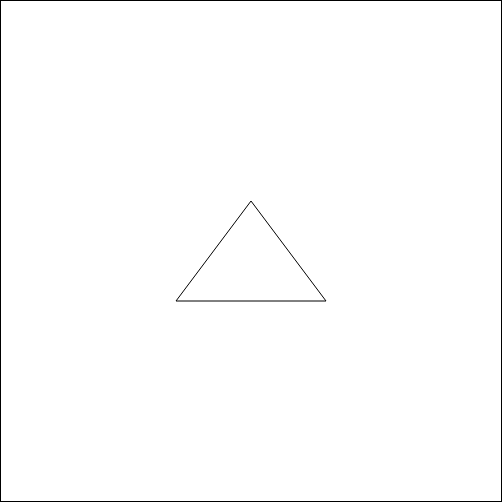
\includegraphics[width=0.9\textwidth]{slike/1_OsnovniCanvasTrokut.png}
    \captionsetup{justification=centering}
    \caption{Prikaz jednostavnog trokuta koristeći Canvas API}
\label{fig:OsnovniCanvasTrokut}
\end{figure}

Kao što se vidi iz slike \ref{fig:OsnovniCanvasTrokut}, trokut se nalazi približno na sredini platna, no Canvas API nema funkcije za centriranje crteža. U kodu je definirano da je platno široko i visoko 500 piksela na temelju čega su određene okvirne koordinate trokuta. Slijedi da se koordinatni sustav platna kreće od 0 do 500 u visini i u širini gdje je točka $(0,0)$ gornji lijevi kut, a točka $(500,500)$ donji desni kut. Problem nastaje kada je potrebno definirati trokut na koordinatama koje su manje od 0, a veće od 500 piksela. Dodatno, teško je crtati objekte u sustavu koji je uvijek ograničen veličinom platna u pikselima i koji ne može sadržavati negativne brojeve. Ove koordinate platna još se nazivaju i zaslonske koordinate.

\section{Lokalne, globalne i zaslonske koordinate}

Lokalne, globalne i zaslonske su termini koji opisuju različite poglede na korištene koordinate. Kako je već spomenuto prije, zaslonske koordinate nisu previše praktične za rad zbog čega se uvodi pojam lokalnih i globalnih koordinata. Transformacija iz jedne vrste koordinata u drugu je jednostavna i nužna za lakši rad s grafikom. 

Lokalne koordinate predstavljaju koordinate nekog objekta unutar njegovog lokalnog referentnog sustava. Time se omogućava upravljanje objektom neovisno o njegovom položaju u globalnom sustavu. Pojednostavljeno, to su koordinate objekta koje su najjednostavnije za upravljanje jer ne ovise ni o čemu osim o odabranom sustavu u kojem je definiran. Te koordinate su najčešće povezane s ishodištem koordinatnog sustava. Na primjer, lokalne koordinate nekog trokuta se mogu definirati tako da se jedan od vrhova trokuta nalazi u ishodištu koordinatnog sustava. To olakšava kasnije upravljanje položajem trokuta jer se svaka transformacija događa u odnosu na ishodište. Na slici \ref{fig:LokalneKoordinateTrokut} prikazan je trokut definiran lokalnim koordinatama.
\\
\begin{figure}[H]
    \centering
    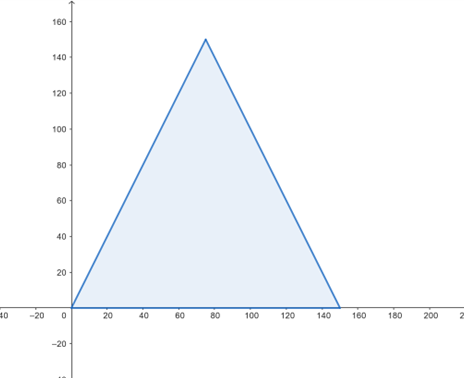
\includegraphics[width=0.9\textwidth]{slike/2_LokalneKoordinateTrokut.png}
    \captionsetup{justification=centering}
    \caption{Prikaz trokuta definiranog lokalnim koordinatama}
\label{fig:LokalneKoordinateTrokut}
\end{figure}

Globalne koordinate su koordinate objekta u odnosu na cijeli prostor, a koristi referentni sustav koji je zajednički svim objektima u prostoru. Na primjer, ako je potrebno napraviti kompoziciju više objekata, njihove lokalne koordinate se koriste kao temelj za transformaciju u prostoru. Transformacijama se pozicioniraju objekti u zajedničkom prostoru čime se dobivaju globalne koordinate. Na slici \ref{fig:GlobalneKoordinateTrokuti} prikazani su zeleni trokuti definirani svojim globalnim koordinatama. Iscrtan je i crveni trokut definiran svojim lokalnim koordinatama na temelju kojeg su dobiveni svi ostali zeleni trokuti.
\\
\begin{figure}[H]
    \centering
    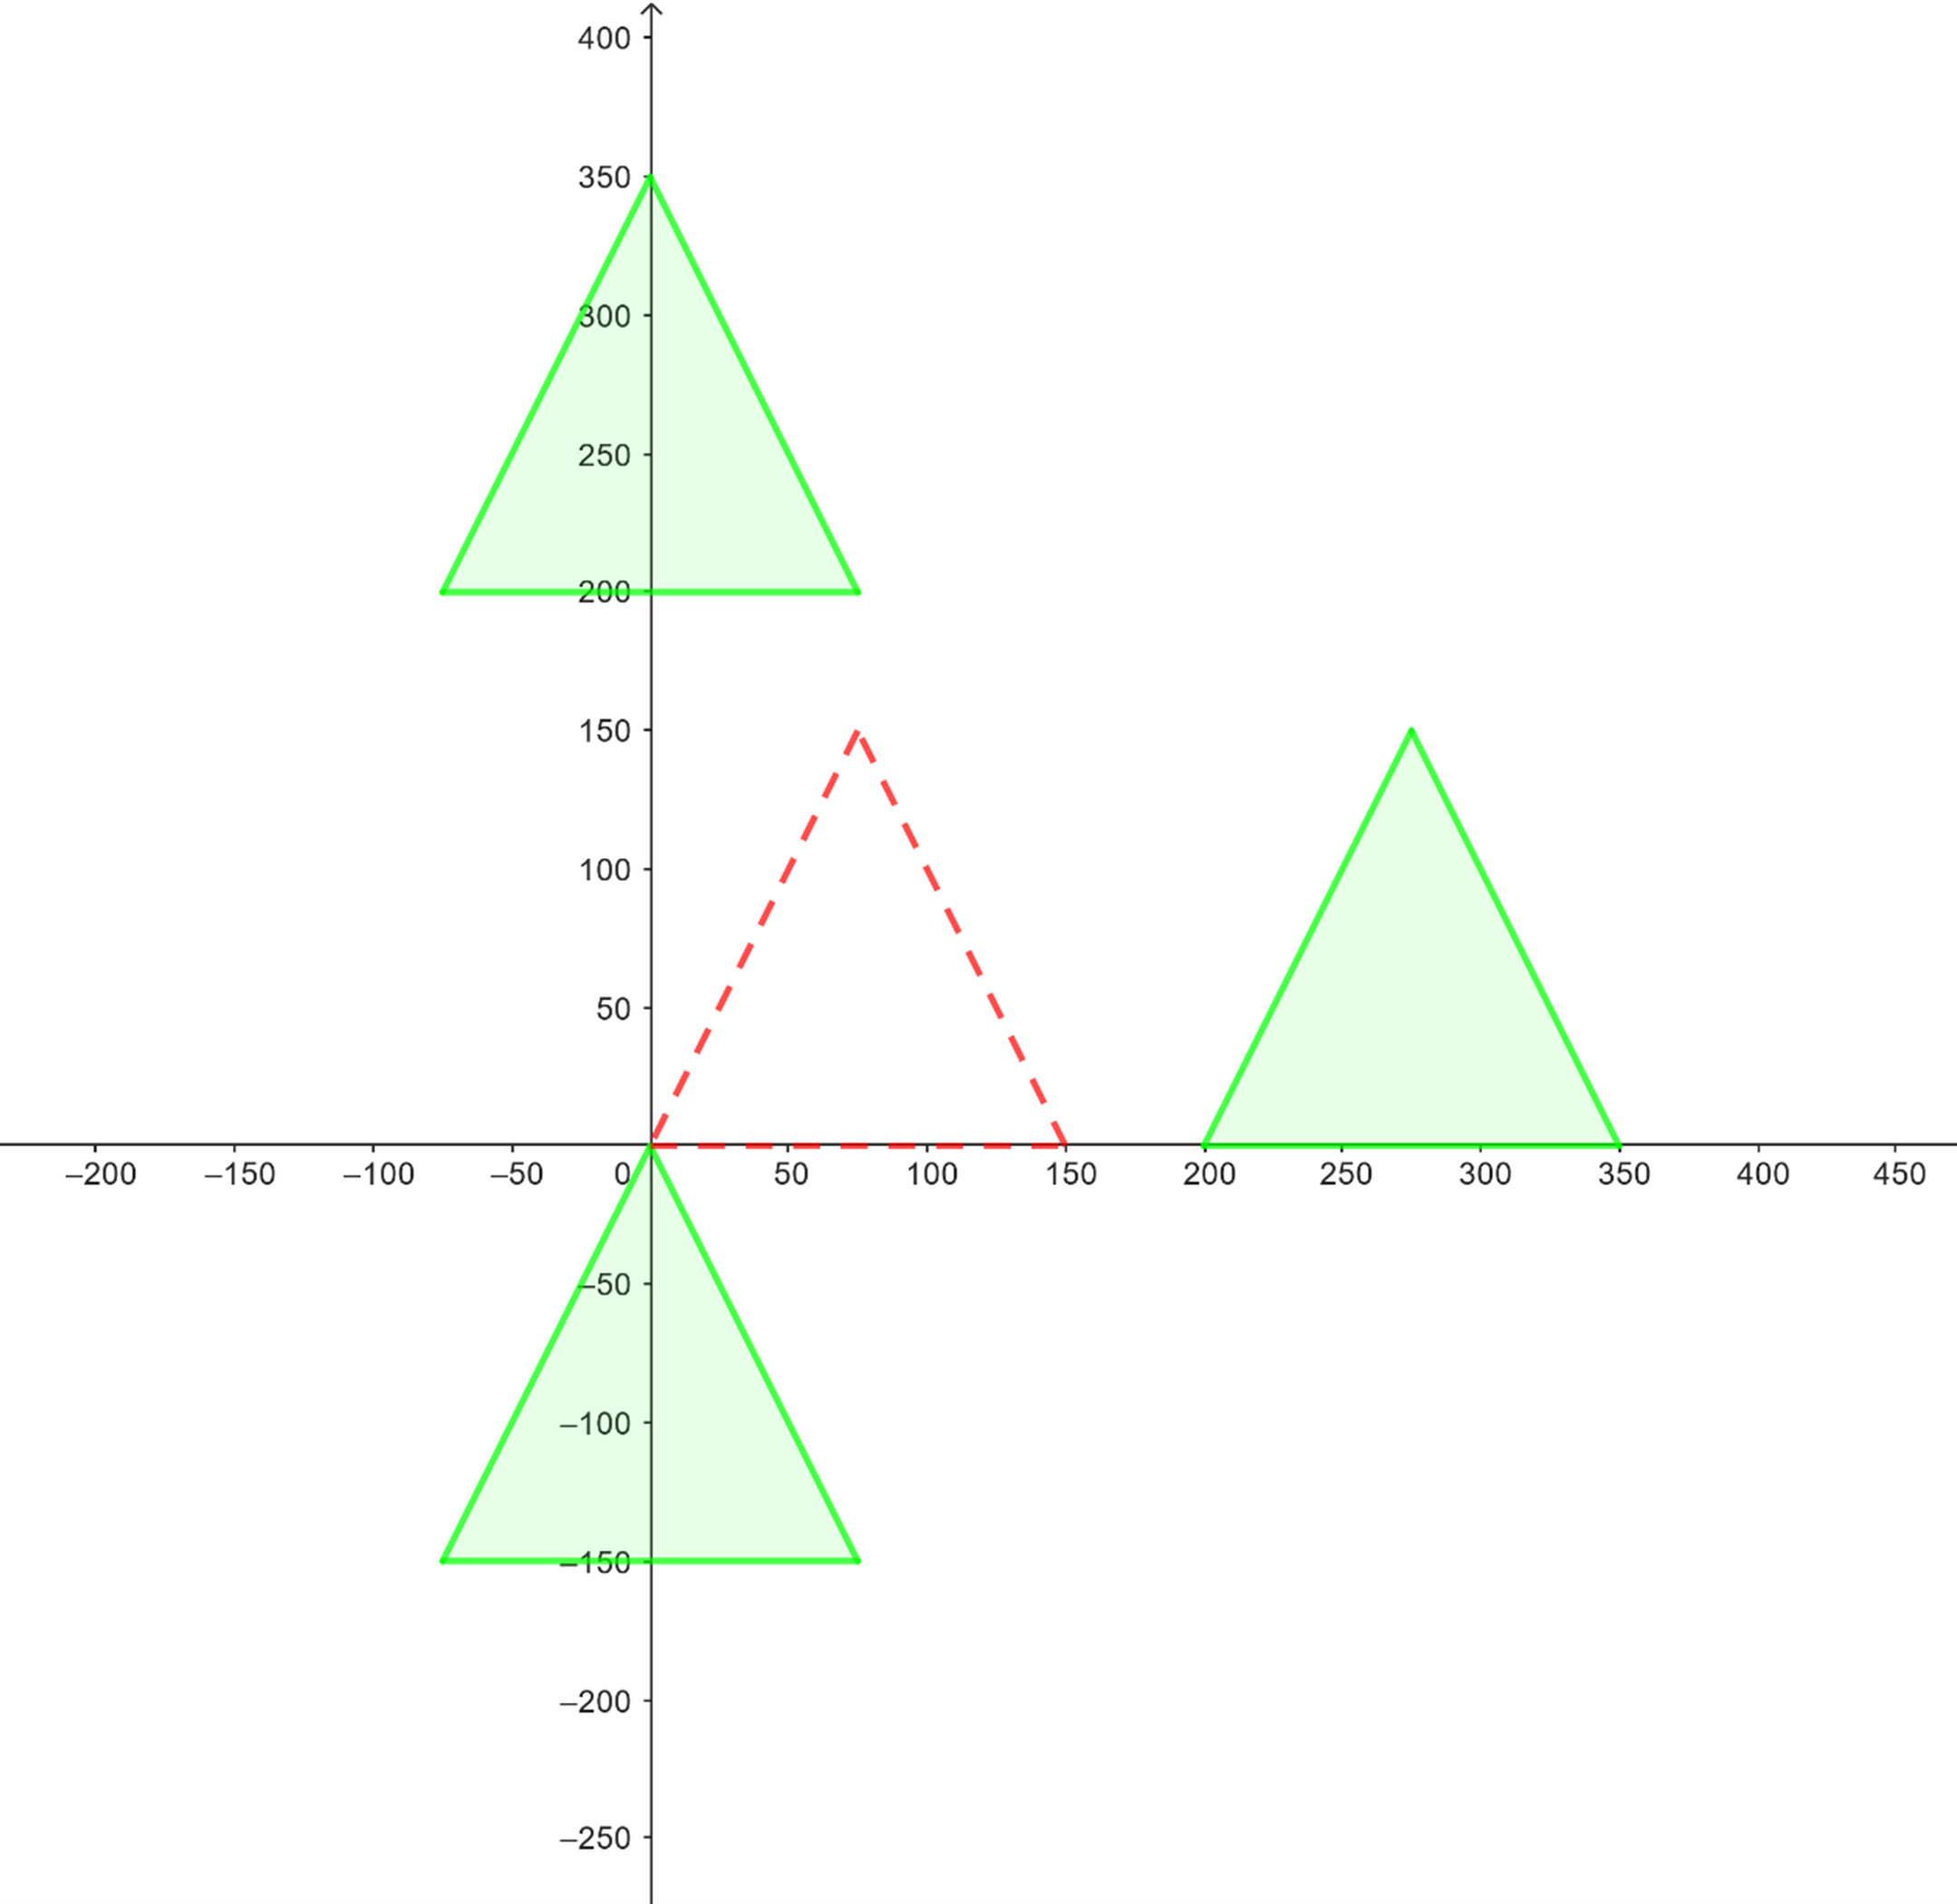
\includegraphics[width=0.9\textwidth]{slike/3_GlobalneKoordinateTrokuti.png}
    \captionsetup{justification=centering}
    \caption{Prikaz trokuta definiranih globalnim koordinatama}
\label{fig:GlobalneKoordinateTrokuti}
\end{figure}

Zaslonske koordinate predstavljaju koordinate objekta u odnosu na zaslon uređaja ili zaslon na kojemu se objekti prikazuju. Najčešće su izražene u pikselima. Trokuti definirani globalnim koordinatama iz slike \ref{fig:GlobalneKoordinateTrokuti} se mogu prikazati na ekranu koristeći njihove globalne koordinate, no tako bi se dobio neželjeni efekt. Na slici \ref{fig:ZaslonskeKoordinateCanvas} prikazani su trokuti sa slike \ref{fig:GlobalneKoordinateTrokuti} nacrtani na platnu bez da su prije transformirani u zaslonske koordinate. 
\begin{figure}[H]
    \centering
    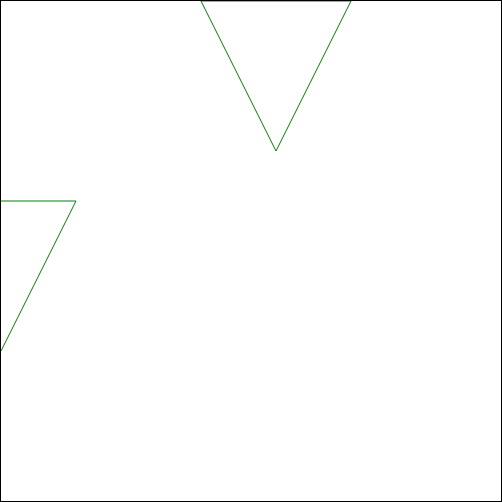
\includegraphics[width=0.9\textwidth]{slike/4_ZaslonskeKoordinateCanvas.png}
    \captionsetup{justification=centering}
    \caption{Prikaz trokuta definiranih globalnim koordinatama unutar platna}
\label{fig:ZaslonskeKoordinateCanvas}
\end{figure}

Trokuti sa slike \ref{fig:ZaslonskeKoordinateCanvas} se nalaze izvan platna i svi su obrnuti. To je zato što globalni koordinatni sustav ima $y$ os čije vrijednosti rastu "prema gore", a platno ima $y$ os čije vrijednosti rastu "prema dole". Osim toga, koordinate nekih trokuta su izvan intervala visine i širine od $[0, 500]$. Zbog razlika između sustava u kojem je objekt definiran i sustava na kojemu se objekt prikazuje, potrebno je napraviti transformacije koordinata. Tako se od globalnih koordinata objekta dolazi do njegovih zaslonskih koordinata \parencite{MediumCoords2023}.

Potrebno je trokute sa slike \ref{fig:GlobalneKoordinateTrokuti} nacrtati unutar platna. Dio slike \ref{fig:GlobalneKoordinateTrokuti} koji je potrebno nacrtati se može ograničiti tako da se prikažu sve točke od -400 do 400 na $x$ i $y$ osi na platnu koje je ograničeno na $x$ i $y$ osi od 0 do 500. Za to je potrebno prvo skalirati koordinatni sustav trokuta da bude jednake veličine kao i koordinatni sustav zaslona. Nakon toga, potrebno je pomaknuti koordinatni sustav trokuta tako da se podudara s granicama koordinatnog sustava zaslona. Ukratko, potrebno je skalirati i pomaknuti sve točke tako da stanu u zacrtane okvire platna. Formule za te transformacije su relativno jednostavne:

\begin{align*}
x' = \left(\frac{w}{x_{\max} - x_{\min}}\right) \cdot x - \left(\frac{w}{x_{\max} - x_{\min}}\right) \cdot x_{\min}
\\
\\
y' = \left(\frac{-h}{y_{\max} - y_{\min}}\right) \cdot y - \left(\frac{-h}{y_{\max} - y_{\min}}\right) \cdot y_{\max}
\end{align*}

 gdje su $x_{min}$, $x_{max}$, $y_{min}$ i $y_{max}$  granice koordinatnog sustava trokuta, $w$ i $h$ su širina i visina platna na kojemu će se trokuti prikazati, $x$ i $y$ su globalne koordinate točke koju je potrebno prikazati na zaslonu i na kraju, $x'$ i $y'$ predstavljaju zaslonske koordinate te točke. Varijable $x_{min}$ i $y_{min}$ predstavljaju najnižu, a $x_{max}$ i $y_{max}$ najvišu vrijednost koja se može prikazati na $x$ i $y$ osi. Formule je lakše pojasniti ako se rastave na više manjih dijelova:

\begin{align*}
s_x = \frac{w}{x_{\max} - x_{\min}}
\\
\\
s_y = -\frac{h}{y_{\max} - y_{\min}}
\\
\\
p_x = -s_x \cdot x_{\min}
\\
\\
p_y = -s_y \cdot y_{\max}
\\
\\
x' = s_x \cdot x + p_x
\\
\\
y' = s_y \cdot y + p_y.
\end{align*}

Ovdje $s_x$ i $s_y$ predstavljaju koeficijente koji označavaju koliko puta su širina i visina zaslona veće od širine i visine dijela koordinatnog sustava u kojemu su definirani trokuti. Množenjem globalnih koordinata tim koeficijentima skalira se vizualizacija trokuta tako da oni stanu unutar zaslona na kojemu će se prikazivati. Prikaz na zaslonu  bez ikakvih transformacija prikazan je na slici \ref{fig:GlobalniTrokutiUnutarZaslona}. Rezultat nakon skaliranja prikazan je na slici \ref{fig:SkaliraniGlobalniTrokutiUnutarZaslona}. Dio ekrana koji nije precrtan linijama predstavlja zaslon.

\begin{figure}[H]
    \centering
    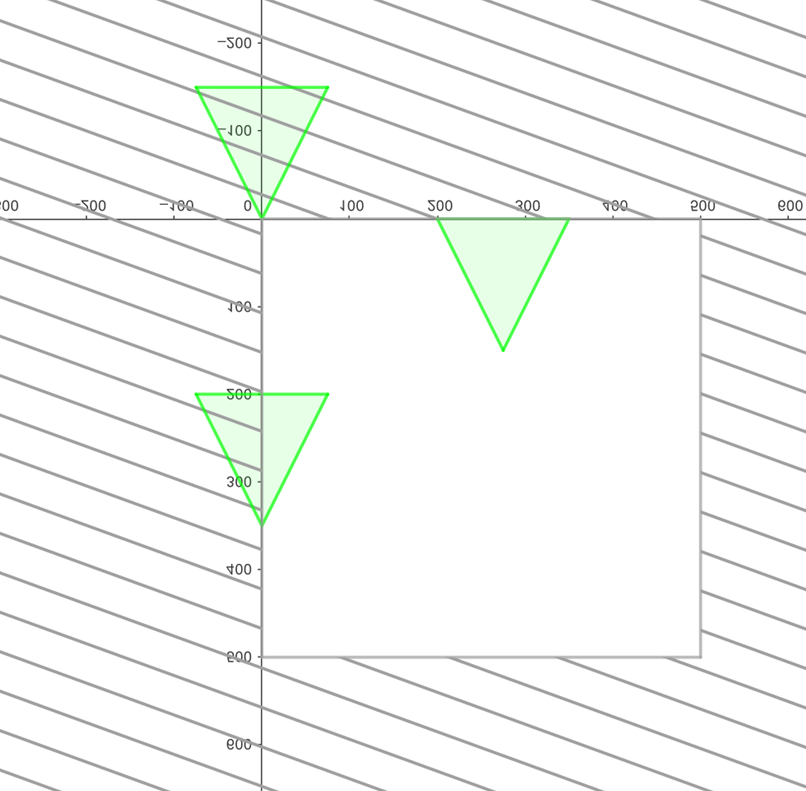
\includegraphics[width=1\textwidth]{slike/5_GlobalniTrokutiUnutarZaslona.png}
    \captionsetup{justification=centering}
    \caption{Prikaz trokuta definiranih globalnim koordinatama}
\label{fig:GlobalniTrokutiUnutarZaslona}
\end{figure}
\begin{figure}[H]
    \centering
    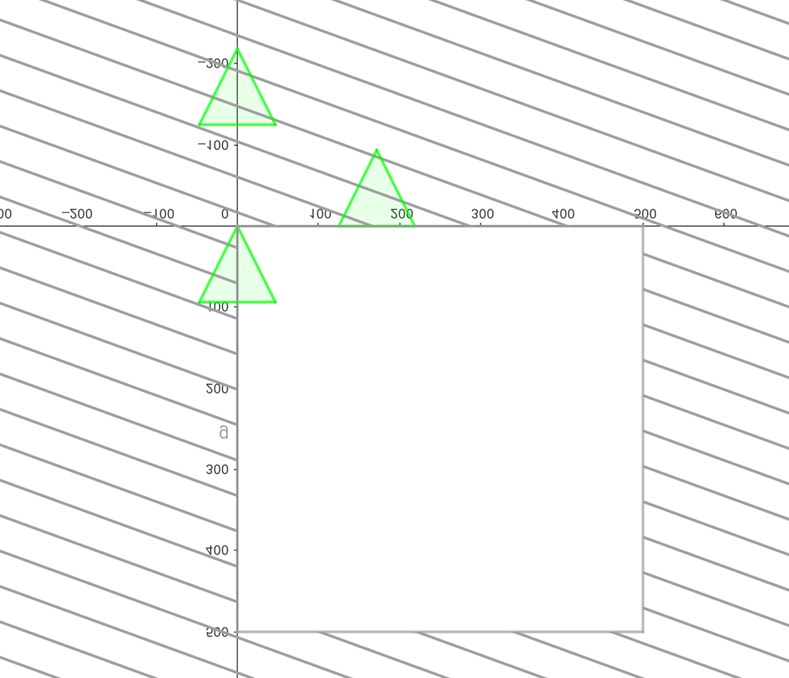
\includegraphics[width=0.9\textwidth]{slike/6_SkaliraniGlobalniTrokutiUnutarZaslona.png}
    \captionsetup{justification=centering}
    \caption{Prikaz trokuta sa skaliranim globalnim koordinatama}
\label{fig:SkaliraniGlobalniTrokutiUnutarZaslona}
\end{figure}


Najočitija razlika sa slika \ref{fig:GlobalniTrokutiUnutarZaslona} i \ref{fig:SkaliraniGlobalniTrokutiUnutarZaslona} je ta što su trokuti odjednom okrenuti u pravome smjeru. Do toga je došlo zbog dodanog minusa u formuli za dobivanje $s_y$ koeficijenta. Kao što je spomenuto ranije, $y$ os platna se kreće u suprotnome smjeru, odnosno raste od gore prema dole zbog čega je bilo potrebno "okrenuti" $y$ os. Dalje je potrebno pomaknuti sve trokute tako da budu unutar okvira zaslona. Varijable $p_x$ i $p_y$ predstavljaju pomak koji je potrebno napraviti kako bi se rubovi koordinatnih sustava podudarali. Finalni rezultat prikazan je na slici \ref{fig:TransformiraneGlobalneUZaslonske}. 

\begin{figure}[H]
    \centering
    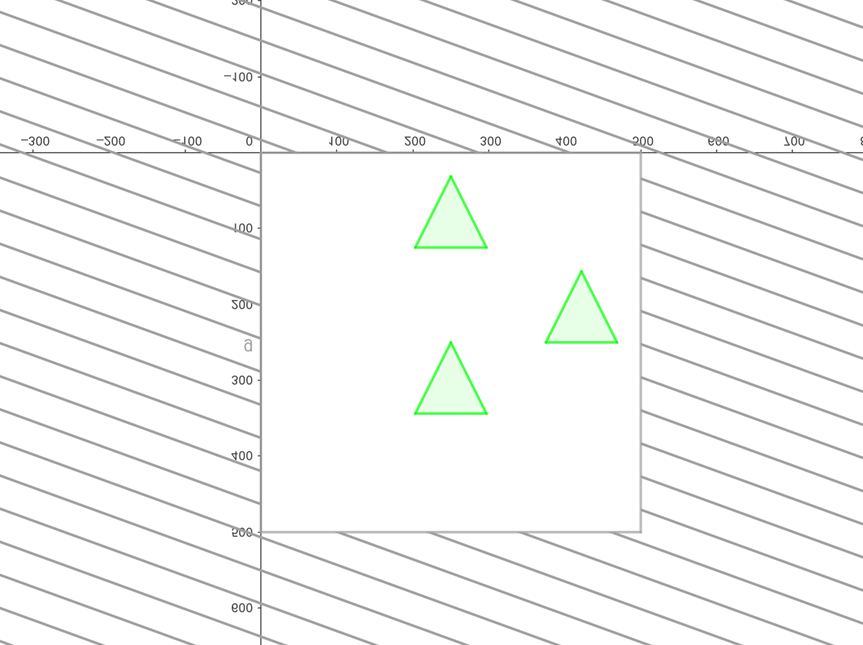
\includegraphics[width=0.9\textwidth]{slike/7_TransformiraneGlobalneUZaslonske.png}
    \captionsetup{justification=centering}
    \caption{Nacrtani trokuti nakon transformacije koordinata}
\label{fig:TransformiraneGlobalneUZaslonske}
\end{figure}

Transformacije koordinata se mogu primijeniti na koordinate trokuta sa slike \ref{fig:ZaslonskeKoordinateCanvas}. Klasa \textit{GlobalniKoordinatniSustav} će služiti za provođenje tih transformacija. Ona će kao parametre primati platno za crtanje, $x_{min}$, $x_{max}$, $y_{min}$ i $y_{max}$, a pri svakom pozivu metoda za crtanje će vršiti transformaciju koordinata iz globalnih u zaslonske. Klasa \textit{GlobalniKoordinatniSustav} će kasnije biti izdvojena u zasebnu datoteku, a određene metode će biti uklonjene jer neće biti potrebne. \parencite{HipHorvatUvod}. 

Primjena klase \textit{GlobalniKoordinatniSustav} na primjeru sa slike \ref{fig:ZaslonskeKoordinateCanvas} prikazana je na slici \ref{fig:TransformiraniTrokutiCanvas}.

\begin{figure}[H]
    \centering
    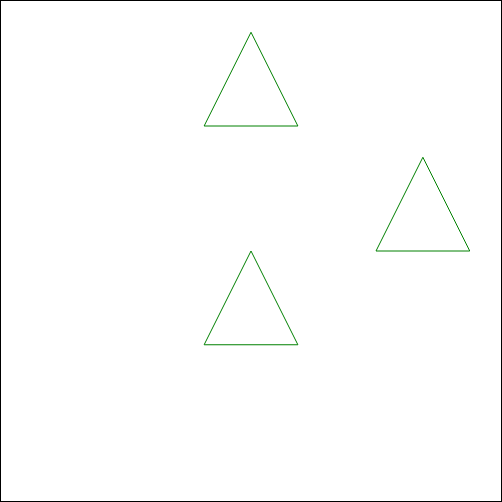
\includegraphics[width=0.9\textwidth]{slike/8_TransformiraniTrokutiCanvas.png}
    \captionsetup{justification=centering}
    \caption{Crtanje trokuta primjenom klase \textit{GlobalniKoordinatniSustav}}
\label{fig:TransformiraniTrokutiCanvas}
\end{figure}

\chapter{2D vizualizacije}
Nakon uvodnog pregleda osnovnih koncepata potrebnih za crtanje na platnu, može se krenuti u razradu vizualizacije eksplozije čestica. Prije definiranja kretanja čestica, njihove boje na ekranu i drugih pojedinosti, potrebno je prvo definirati model čestice i kako će on biti predstavljen u kodu. Nakon toga, potrebno je osmisliti način na koji će se čestice generirati, pohranjivati i prikazivati na ekranu, a da se one mogu i micati. 

\section{Jednostavni model čestice}
 Konceptualno, čestica se može zamisliti kao točka na ravnini. Kako je cilj generirati što veći broj čestica, podaci koji predstavljaju česticu bi trebali biti minimalni. Čestice će se prikazivati u dvije dimenzije, zbog čega je dovoljno definirati samo njene dvije prostorne komponente, odnosno njene komponente na $x$ i $y$ osi. Najlakši način za predstavljanje pozicije je korištenje vektora pozicije $\vec{r}$. Kako se vizualizacija eksplozije temelji na kretanju čestica, potrebno je osmisliti kako će kretanje čestice biti predstavljeno. Intuitivno, svakoj čestici treba biti označeno kolikom mjerom se kreće po $x$ osi, a kolikom po $y$ osi. Dakle, potrebno je definirati brzinu kojom se čestica kreće i smjer u kojemu se kreće. Za to je dovoljan jedan vektor smjera $\vec{v}$. Ta brzina mora od nekuda proizlaziti, odnosno mora se djelovati nekom silom na česticu kako bi se mijenjala njena brzina i pozicija. Pojednostavljeno, sila djeluje na česticu čime se mijenja njena brzina, a brzina djeluje na kretanje čestice, odnosno na njenu poziciju u prostoru. Postavlja se pitanje, kako izračunati iduće stanje čestice ako je poznata sila kojom se djeluje na česticu, trenutna brzina i trenutna pozicija čestice?

 Najjednostavnija metoda za dobivanje formule za približni izračun iduće pozicije i brzine čestice koja se kreće određenom brzinom s određene pozicije je Eulerova metoda. Eulerova metoda je numerička metoda za aproksimaciju rješenja diferencijalnih jednadžbi. Unatoč kompliciranim terminima iz definicije, metoda se može vrlo jednostavno objasniti. Pojednostavljeno, diferencijalne jednadžbe su jednadžbe koje kao rješenje nemaju konkretnu varijablu ili broj već funkciju, a Eulerova metoda je način za pronalaženje tih rješenja. Ukratko, Eulerovom metodom se može doći do metode za aproksimaciju pozicije i brzine čestice nakon nekog vrlo malog vremenskom intervala. Taj interval se još naziva i "korak", a najčešće se označava oznakom $dt$. Eulerovom metodom se zapravo pokušavaju pronaći funkcije koje će za danu silu, brzinu i poziciju točke vratiti okvirnu poziciju i brzinu čestice nakon $dt$ sekundi.

Eulerova metoda pretpostavlja da je vrijednost funkcije nakon nekog ekstremno malog vremenskog intervala jednaka zbroju vrijednosti funkcije s početka intervala i umnošku vremenskog intervala s mjerom promjene te funkcije  na početku tog intervala. Na primjer, pretpostavimo da se vlak kreće određenom brzinom u trenutku u kojemu ga promatramo i ta brzina je egzaktno poznata. Osim toga, izmjereno je i ubrzanje vlaka i poznato je koliko je ubrzanje u trenutku u kojemu se promatra vlak. Iz nekog razloga, potrebno je znati kolika će biti brzina vlaka nakon 0.00001 sekundi. Dodatno, poznato je da se ubrzanje može predstaviti kao promjena brzine kroz vrijeme, odnosno postoji direktna veza između trenutne brzine, trenutnog ubrzanja i vremena. Sada je poznata vrijednost funkcije s početka intervala, poznat je korak $dt$ i poznata je mjera promjene funkcije na početku intervala. Tada je dovoljno trenutnoj brzini dodati trenutno ubrzanje pomnoženo s 0.00001 sekundi i dobiva se brzina vlaka nakon 0.00001 sekundi od promatranja. Vrlo je bitno za reći da se ovim postupkom ne dobiva egzaktna brzina, već dovoljno dobra aproksimacija. Koristeći Eulerovu metodu, mogu se izvesti potrebne formule za određivanje pozicije i brzine čestice nakon nekog vrlo malog vremenskog koraka \parencite{EulersMethod2013}.

 Za početak, potrebno je pronaći funkciju na temelju koje se može odrediti samo brzina čestice nakon određenog vremenskog korak $dt$. Izvod te formule temelji se na Newtonovom drugom zakonu i primjeni Eulerove metode. Newtonov drugi zakon govori da je sila koja djeluje na neki objekt jednaka masi tog objekta pomnožena s ubrzanjem istog objekta. Poznatije, taj zakon se zapisuje kao:
 \begin{align*}
F = m \cdot a
\end{align*}
gdje je $F$ sila koja djeluje na objekt, $m$ je njegova masa i $a$ ubrzanje. Iz ove formule može se zaključiti da je akceleracija proporcionalna sili podijeljenoj s masom objekta, odnosno:
 \begin{align*}
a = \frac{F}{m}
\end{align*}
Tako s porastom sile raste ubrzanje, a s porastom mase ono pada.  S druge strane, ubrzanje se može opisati i kao promjena brzine kroz vrijeme, odnosno:
 \begin{align*}
a(t) = \frac{dv(t)}{dt}
\end{align*}
gdje je $a(t)$ ubrzanje objekta u trenutku $t$, $dv(t)$ je ekstremno mala promjena brzine u danom trenutku $t$ i $dt$ je ekstremno mali vremenski interval. Općenito, oznaka $d$ ispred neke varijable označava vrlo malu promjenu u veličini te varijable, u ovom slučaju brzine $v$ i vremena $t$. Sada je napokon dobivena veza između promjene brzine i promjene vremena, a ona glasi:
 \begin{align*}
dv(t) = a(t) \cdot dt.
\end{align*}
Sada je moguće iskoristiti trik iz Eulerove metode, a to je da se umjesto $dv(t)$ uvrsti $\Delta v$. Oznaka $\Delta v$ predstavlja određenu vrijednost, razliku između dviju vrijednosti brzina preko vremenskog intervala $dt$. Do sada su formule predstavljale egzaktnu vezu između varijabli. Eulerova metoda pretpostavlja da je mjera promjene veličine uvijek linearna, no to ne mora uvijek biti tako. Iz tog razloga, počinje se pričati o aproksimacijama, a ne o egzaktnim vrijednostima. Ta aproksimacija se može zapisati kao:
 \begin{align*}
\Delta v \approx a(t) \cdot dt.
\end{align*}
Kako bi u formulu uveli djelovanje sile na brzinu, potrebno je supstituirati ubrzanje s formulom koja je prikazana u prvim koracima ovog izvoda, odnosno:
 \begin{align*}
\Delta v \approx \frac{F(t)}{m} \cdot dt.
\end{align*}
Na kraju, primjenjuje se Eulerova metoda. Time se dolazi do toga da se brzina nakon vremenskog koraka $dt$ (kraće zapisano $v(t + \Delta t)$) može dobiti zbrajanjem trenutne brzine $v(t)$ i umnoška vremenskog koraka $dt$ s mjerom promjene brzine u trenutku $t$ (odnosno njenog ubrzanja $a(t)$) \parencite{HjorthJensen2021}. Potrebna formula za određivanje brzine čestice nakon nekog vremena je:
 \begin{align*}
v(t + \Delta t) \approx v(t) + \frac{F(t)}{m} \cdot dt.
\end{align*}

Na isti način se može dobiti i formula za određivanje pozicije čestice nakon nekog vrlo malog vremenskog intervala. Ako je poznato da je brzina $v(t)$ promjena pozicije $r$ kroz vrijeme $t$, može se izvesti formula:
 \begin{align*}
v(t) = \frac{dr(t)}{dt}.
\end{align*}
Nadalje, aproksimacija dobivena Eulerovom metodom glasi:
 \begin{align*}
\Delta r \approx v(t) \cdot dt,
\end{align*}
a na kraju se dobiva formula:
 \begin{align*}
r(t + \Delta t) \approx r(t) + v(t) \cdot dt.
\end{align*}
Kao što se vidi iz dobivenih formula, u model čestice je potrebno uvrstiti i masu čestice kako bi se moglo vizualizirati njeno kretanje. Svi prikazani koncepti su objašnjeni bez previše spominjanja kalkulusa i nekih osnovnih koncepata matematike. Sama srž teorije nije toliko bitna, bitno je samo razumijevanje Eulerove metode i kako su dobivene potrebne formule \parencite{HipHorvatFizika}.

Potrebno je objašnjene koncepte iskoristiti u JavaScript kodu. Za početak, definirana je klasa \textit{Vektor2D}. U njoj, definirane su osnovne operacije s vektorima kao što su zbrajanje, oduzimanje, množenje skalarom i naravno metoda \textit{dodajCputaV(c,v)}. Metoda \textit{dodajCputaV(c,v)} će se koristiti za implementaciju ranije dobivenih formula.

Klasa \textit{Vektor2D} potrebna je za implementaciju materijalne točke. Materijalna točka je točka u prostoru na koju se može djelovati silom. U njoj su definirani vektori za poziciju i brzinu te masa materijalne točke. Također, u klasi \textit{MaterijalnaTocka} je implementirana metoda \textit{pomakni(dt, rezultantnaSila)} za pomicanje čestice koja se temelji na ranije izvedenim formulama. Cijeli kod za klasu glasi:

\begin{minted}{js}
class MaterijalnaTocka {
  constructor(masa, rVektor, vVektor) {
    this.masa = masa;
    this.r = rVektor;
    this.v = vVektor;
  }

  pomakni(dt, rezultantnaSila) {
    this.v.dodajCputaV(dt / this.masa, rezultantnaSila);
    this.r.dodajCputaV(dt, this.v);
  }
}
\end{minted}

Dalje, potrebno je osmisliti kako će čestica biti prikazana na platnu i kako će se kretati po ekranu. Za to, potrebno je definirati novu klasu za crtanje čestice i modificiranje klase \textit{GlobalniKoordinatniSustav}. 

\section{Vizualizacija čestice i njenog kretanja}
Čestica se najjednostavnije može prikazati kao kvadrat ili kružnica. Kako se radi o česticama, kružnice bi mogle biti vizualno zanimljivije, no oblik čestice zapravo nije ni toliko bitan. Razlog tomu je što se želi smanjiti veličina čestice tako da izgleda kao vrlo mala točka na ekranu, a zbog toga je teško za razlučiti radi li se o kvadratu ili kružnici. Kako je oblik trenutno nebitan, čestica će se vizualizirati kao vrlo mali kvadrat zbog jednostavnosti koda za njegovo crtanje. Dodatno, kako bi se postigla zanimljivija vizualizacija, čestice će biti jarke žute boje, a pozadina platna će biti crna kako bi se čestice bolje razlučile. Za potrebe crtanja čestice napravljena je klasa \textit{Cestica}. Unutar klasa nalazi se referenca na objekt klase \textit{MaterijalnaTocka}. Osim toga, definirana je boja i promjer vizualizacije. Promjer ne određuje izgled čestice, već služi kao bitan atribut koji se koristi u metodi \textit{zarobi(gks, top, right, bottom, left)}. Pomoću metode \textit{zarobi(gks, top, right, bottom, left)} može se vizualizirati odbijanje čestice od granica platna tako da su čestice "zarobljene" u platnu. Druga bitna metoda je metoda \textit{iscrtaj(gks)}. Njoj se prosljeđuje objekt klase \textit{GlobalniKoordinatniSustav} koja crta česticu. Za to, potrebno je klasi \textit{GlobalniKoordinatniSustav} dodati metodu \textit{piksel(x, y, boja} koja crta vrlo mali kvadrat koji izgleda kao piksel. Bitno je za napomenuti kako ta metoda ne crta zapravo piksel jer bi njega bilo teško za vidjeti, iako se tako zove. Dodana metoda izgleda ovako:

\begin{minted}{js}
  piksel(x, y, boja) {
    this.g.fillStyle = boja;
    this.g.fillRect(this.sx * x + this.px, this.sy * y + this.py, 1, 1);
  }
\end{minted}

Klasa \textit{Cestica} definirana je u kodu s konstruktorom i dvije metode:

\begin{minted}{js}
class Cestica {
  constructor(promjer, materijalnaTocka, boja = "yellow") {
    this.materijalnaTocka = materijalnaTocka;
    this.boja = boja;
    this.promjer = promjer;
  }

  zarobi(gks, top = true, right = true, bottom = true, left = true) {
    if (this.materijalnaTocka.r.x < gks.xmin + this.promjer && left) {
      this.materijalnaTocka.v.x = -this.materijalnaTocka.v.x;
    }
    if (this.materijalnaTocka.r.x > gks.xmax - this.promjer && right) {
      this.materijalnaTocka.v.x = -this.materijalnaTocka.v.x;
    }
    if (this.materijalnaTocka.r.y < gks.ymin + this.promjer && bottom) {
      this.materijalnaTocka.v.y = -this.materijalnaTocka.v.y;
    }
    if (this.materijalnaTocka.r.y > gks.ymax - this.promjer && top) {
      this.materijalnaTocka.v.y = -this.materijalnaTocka.v.y;
    }
    if (this.materijalnaTocka.r.y < gks.ymin + this.promjer && bottom) {
      this.materijalnaTocka.r.y = gks.ymin + this.promjer;
    }
  }

  iscrtaj(gks) {
    gks.piksel(this.materijalnaTocka.r.x, this.materijalnaTocka.r.y, this.boja);
  }
}
\end{minted}
Napokon, moguće je nacrtati česticu i njenu putanju. Za početak, na slici \ref{fig:CesticaNaPlatnu} je prikazana jedna čestica na platnu. Njena vektor brzine je $(0, 0)$ i nema putanju po kojoj se kreće. Čestica je žute boje, a dodatno je označena crvenom kružnicom kako bi se lakše vidjela. Skripta za vizualizaciju je vrlo jednostavna:

\begin{minted}{js}
  function main() {
    let canvas = document.getElementById("canvas");
    let gks = new GlobalniKoordinatniSustav(canvas, -10, 10, -10, 10);

    let cestica = new Cestica(
      0.1,
      new MaterijalnaTocka(1, new Vektor2D(-4, -4), new Vektor2D(0, 0))
    );

    cestica.iscrtaj(gks);
  }

  window.onload = main;
\end{minted}

\begin{figure}[H]
    \centering
    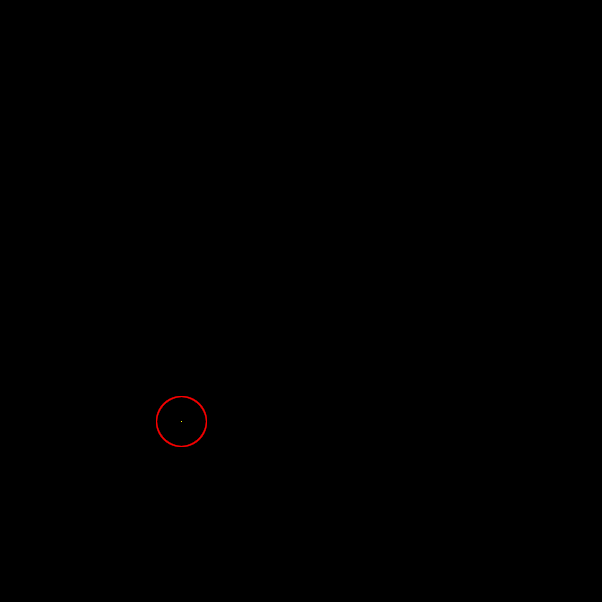
\includegraphics[width=0.9\textwidth]{slike/9_CesticaNaPlatnu.png}
    \captionsetup{justification=centering}
    \caption{Prikaz jedne stacionarne čestice}
\label{fig:CesticaNaPlatnu}
\end{figure}

Za crtanje putanje, potrebno je definirati vremenski korak $dt$ i vektor brzine čestice. Definirana je \textit{for} petlja u kojoj čestica prvo pomakne, zatim se nacrta i na kraju se provjerava odbija li se čestica od neke granice platna. Petlja se izvršava 1000 puta tako da će biti prikazana putanja čestice u intervalu od 250 sekundi. Putanja čestice je prikazana na slici \ref{fig:PutanjaCestice}. Kako nijedna sila ne utječe na česticu, čestica će se kretati konstantnom brzinom i odbiti će se od granice bez usporavanja. Kod za simulaciju naveden je ispod:

\begin{minted}{js}
  function main() {
    let canvas = document.getElementById("canvas");
    let gks = new GlobalniKoordinatniSustav(canvas, -10, 10, -10, 10);

    let cestica = new Cestica(
      0.1,
      new MaterijalnaTocka(1, new Vektor2D(-4, -4), new Vektor2D(1, -2))
    );

    let dt = 0.25;
    for (let i = 0; i < 1000; i++) {
      cestica.materijalnaTocka.pomakni(dt, new Vektor2D(0, 0));
      cestica.iscrtaj(gks);
      cestica.zarobi(gks, false, false, true, false);
    }
  }
  
  window.onload = main;
\end{minted}
\begin{figure}[H]
    \centering
    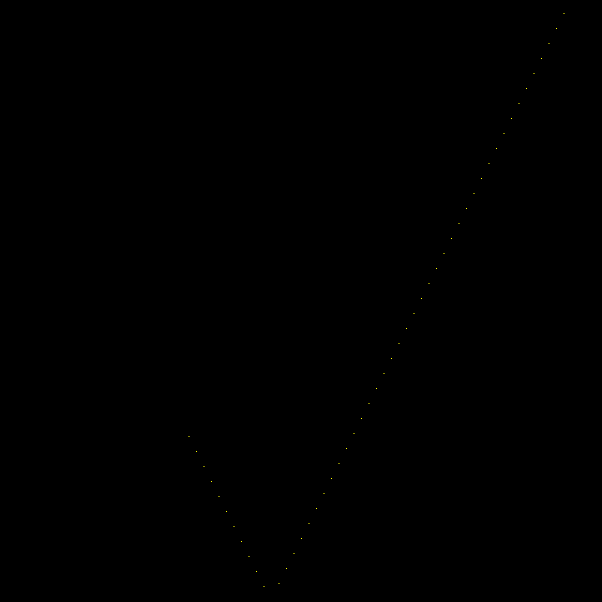
\includegraphics[width=0.9\textwidth]{slike/10_PutanjaCestice.png}
    \captionsetup{justification=centering}
    \caption{Prikaz putanje čestice}
\label{fig:PutanjaCestice}
\end{figure}

U stvarnim sustavima na Zemlji, kretanje čestice nije potpuno nesputano. Kako je cilj postizanje što realističnije eksplozije, potrebno je uračunati dodatne čimbenike koji mogu utjecati na kretanje čestice. Prvo, čestica se u stvarnom sustavu na Zemlji neće neprekidno kretati, ona će nakon nekog vremena morati stati. Glavni razlog tomu je otpor sredstva kao što su voda ili zrak u kojemu se ona kreće. Sila otpora je sila koja se pojavljuje kada se objekt kreće kroz neko sredstvo i uvijek djeluje suprotno smjeru kretanja. Sila otpora će nakon nekog vremena u potpunosti zaustaviti objekt. Ova sila je predstavljena formulom:
 \begin{align*}
F = -b\cdot v
\end{align*}
Koeficijent $b$ predstavlja koeficijent otpora sredstva, a oznaka $v$ predstavlja brzinu objekta koji se kreće kroz sredstvo \parencite{UTKLabPhys135}. Silu otpora vrlo je lako za implementirati u kodu. Potreban je samo konstruktor kojemu se prosljeđuje koeficijent otpora i metoda \textit{F(materijalnaTocka)} u kojoj se računa vektor sile:

\begin{minted}{js}
class Otpor {
  constructor(o) {
    this.o = o;
  }
  F(materijalnaTocka) {
    return new Vektor2D(
      -this.o * materijalnaTocka.v.x,
      -this.o * materijalnaTocka.v.y
    );
  }
}
\end{minted}
Korištenje ove sile na prijašnjem primjeru sa slike \ref{fig:PutanjaCesticeSOtporom} će rezultirati laganim skraćivanjem putanje čestice, odnosno postepenim zaustavljanjem čestice koja se kreće. Prikaz ovog rezultata nalazi se na slici \ref{fig:PutanjaCesticeSOtporom}. U kodu je bilo dovoljno pozvati skriptu u kojoj je definirana klasa \textit{Otpor}, inicijalizirati objekt klase \textit{Otpor} i pozvati metodu za izračun sile \textit{F(materijalnaTocka)}. Izmijenjeni isječak koda izgleda ovako:

\begin{minted}{js}
...
let otporSredstva = new Otpor(0.1);
let dt = 0.25;
for (let i = 0; i < 1000; i++) {
  const silaOtpora = otporSredstva.F(cestica.materijalnaTocka);
  cestica.materijalnaTocka.pomakni(dt, silaOtpora);
  cestica.iscrtaj(gks);
  cestica.zarobi(gks, false, false, true, false);
}
...
\end{minted}
\begin{figure}[H]
    \centering
    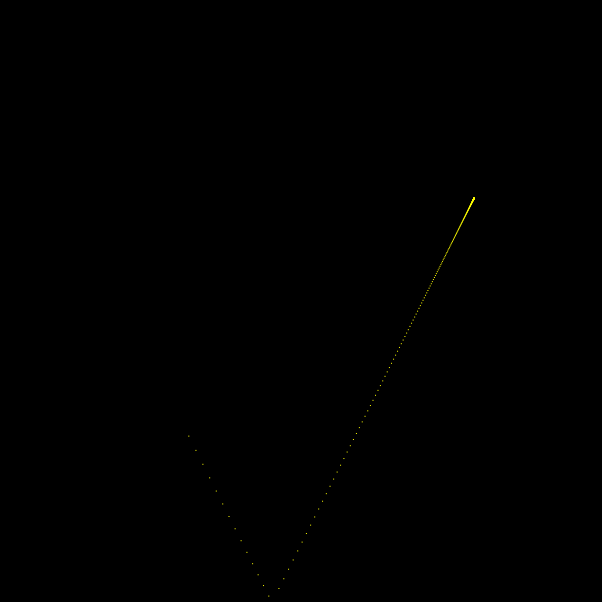
\includegraphics[width=0.9\textwidth]{slike/11_PutanjaCesticeSOtporom.png}
    \captionsetup{justification=centering}
    \caption{Prikaz putanje čestice s otporom}
\label{fig:PutanjaCesticeSOtporom}
\end{figure}

Druga sila koja će se primijeniti na vizualizaciji je sila teža. Djelovanje sile teže na česticu će imati očiti učinak koji će uvelike doprinijeti realizmu vizualizacija. Sila teža zapravo predstavlja rezultantnu silu gravitacijske sile i centrifugalne sile planeta. Ova sila je predstavljena formulom:
 \begin{align*}
F = m\cdot g
\end{align*}
Ovdje $m$ predstavlja masu objekta, a $g$ predstavlja gravitacijsku akceleraciju, odnosno ubrzanje objekta prema planetu. Ova formula je ista kao i za Newtonov drugi zakon, no umjesto akceleracije $a$, uvrštena je gravitacijska akceleracija $g$ \parencite{NASAWeightMass}. 
Na Zemlji, gravitacijska akceleracija je konstanta 9.81, no za potrebe vizualizacije, ona će se moći prilagoditi:
\begin{minted}{js}
class SilaTeza {
  constructor(g) {
    this.g = g;
  }

  F(mt) {
    return new Vektor2D(0, mt.masa * -this.g);
  }
}
\end{minted}

Slika \ref{fig:PutanjaCesticeSilaTeza} prikazuje djelovanje sila teže na česticu. Na slici se vidi kako čestica odskače od donje granice platna, no ona ne usporava jer nema gubitka energije do kojeg dolazi zbog otpora sredstva. Također, pretpostavlja se da je udar savršeno elastičan zbog čega nema ni gubitka energije od udarca u donju granicu platna. U kodu je samo potrebno zamijeniti silu koja djeluje na česticu. Ovdje će se umjesto otpora sredstva, uvrstiti sila teža:

\begin{minted}{js}
...
let silaTeza = new SilaTeza(0.25);
let dt = 0.25;
for (let i = 0; i < 1000; i++) {
  const sila = silaTeza.F(cestica.materijalnaTocka);
  cestica.materijalnaTocka.pomakni(dt, sila);
  cestica.iscrtaj(gks);
  cestica.zarobi(gks, false, false, true, false);
}
...
\end{minted}

\begin{figure}[H]
    \centering
    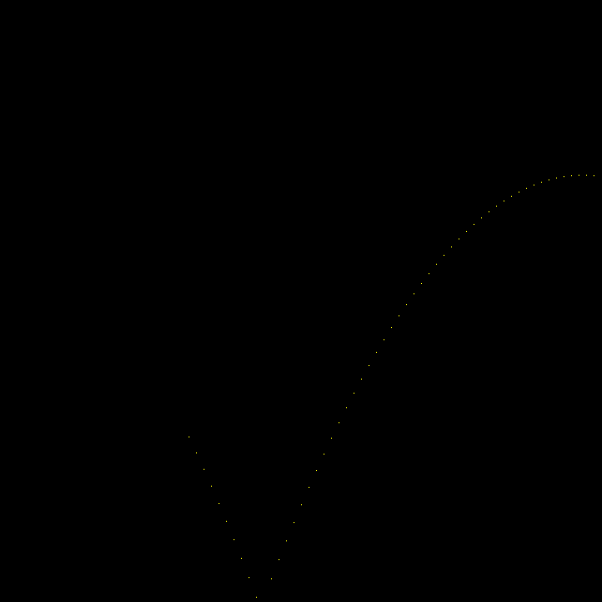
\includegraphics[width=0.9\textwidth]{slike/12_PutanjaCesticeSilaTeza.png}
    \captionsetup{justification=centering}
    \caption{Prikaz putanje čestice na koju djeluje sila teža}
\label{fig:PutanjaCesticeSilaTeza}
\end{figure}
Djelovanje obje sile će dati najrealističniju putanju čestice. Zbrajanjem djelovanja sile teže i otpora sredstva dobiva se zanimljivija vizualizacija. Putanja je prikazana na slici \ref{fig:PutanjaCesticeOtporSilaTeza}. U kodu je potrebno inicijalizirati objekte klasa za otpor sredstva i silu težu i zbrojiti njihove vektore sila. Tada se tom rezultantom silom djeluje na česticu:

\begin{minted}{js}
...

let silaTeza = new SilaTeza(0.25);
let otporSredstva = new Otpor(0.1);
let dt = 0.25;
for (let i = 0; i < 1000; i++) {
  const sila = silaTeza.F(cestica.materijalnaTocka);
  const silaOtpora = otporSredstva.F(cestica.materijalnaTocka);
  cestica.materijalnaTocka.pomakni(dt, sila.zbroji(silaOtpora));
  cestica.iscrtaj(gks);
  cestica.zarobi(gks, false, false, true, false);
}

...
\end{minted}

\begin{figure}[H]
    \centering
    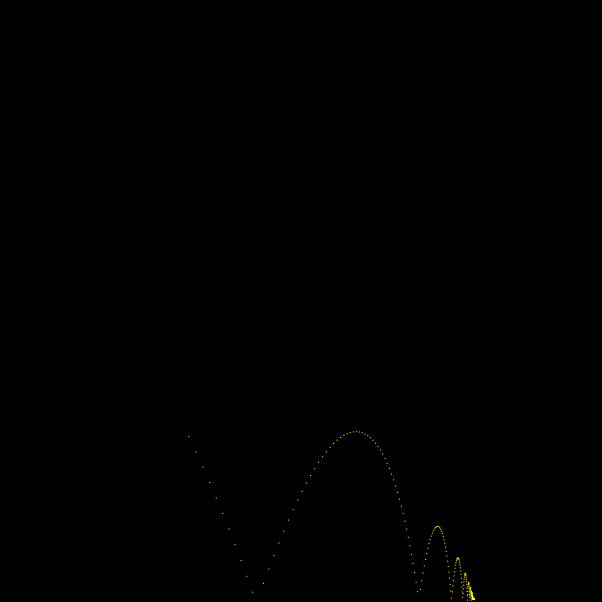
\includegraphics[width=0.9\textwidth]{slike/13_PutanjaCesticeOtporSilaTeza.png}
    \captionsetup{justification=centering}
    \caption{Prikaz putanje čestice s djelovanjem otpora i sile teže}
\label{fig:PutanjaCesticeOtporSilaTeza}
\end{figure}

Crtanje cijele putanje je dovoljno dobar način za prikaz kretanja čestice u prostoru, no realističnije bi bilo prikazati kretanje čestice kao animaciju. Crtanje kretanja čestice se postiže tako da se prvo nacrta čestica, na nju se djeluje silom, promijeni se njena pozicija i zatim se obriše sve nacrtano s platna. Zatim se nacrta nova pozicija čestice i ovaj proces se ponavlja sve dok se vizualizacija ne prekine. Canvas API već ima definiranu metodu za "čišćenje" platna, a JavaScript ima definiranu metodu za izvođenje animacija. Za početak, potrebno je dodati metodu za čišćenje platna u klasu \textit{GlobalniKoordinatniSustav}:

\begin{minted}{js}
  ocisti() {
    let max = this.h;
    if (this.w > this.h) max = this.w;
    this.g.clearRect(0, 0, max, max);
  }
\end{minted}

Dalje, potrebno je pozvati metodu za izvođenje animacije. Metoda \textit{requestAnimationFrame(callback)} označava da se želi izvršavati animacija. Kao parametar, prosljeđuje se metoda koja se koristi za crtanje "sličice" animacije. Najčešće, funkcija koja poziva metodu \textit{requestAnimationFrame(callback)} prosljeđuje sebe kao parametar metodi \textit{requestAnimationFrame(callback)} \parencite{RequestAnimationFrame}. Prije toga, postaviti će se funkcija u kojoj se prvo očisti platno, a zatim se izvode sva potrebna crtanja i poziva se metoda za prikaz idućeg ekrana:

\begin{minted}{js}
  function main() {
    let canvas = document.getElementById("canvas");
    let gks = new GlobalniKoordinatniSustav(canvas, -10, 10, -10, 10);

    let cestica = new Cestica(
      0.1,
      new MaterijalnaTocka(1, new Vektor2D(-4, -4), new Vektor2D(1, -2))
    );

    let silaTeza = new SilaTeza(0.25);
    let otporSredstva = new Otpor(0.1);
    let dt = 0.05;

    function render() {
      gks.ocisti();
      const sila = silaTeza.F(cestica.materijalnaTocka);
      const silaOtpora = otporSredstva.F(cestica.materijalnaTocka);
      cestica.materijalnaTocka.pomakni(dt, sila.zbroji(silaOtpora));
      cestica.iscrtaj(gks);
      cestica.zarobi(gks, false, false, true, false);
      requestAnimationFrame(render);
    }

    render();
  }

  window.onload = main;
\end{minted}
Rezultat izvođenja ovog koda je najbolje prikazati kao "strip" koji se čita s lijeva na desno, a prikazan je na slici \ref{fig:AnimacijaPutanjaCestice}

\begin{figure}[H]
    \centering
    \includegraphics[width=0.95\textwidth]{slike/14_AnimacijaPutanjaCestice.png}
    \captionsetup{justification=centering}
    \caption{Prikaz dijelova animacije kretanja čestice}
\label{fig:AnimacijaPutanjaCestice}
\end{figure}

Napokon, definiran je model čestice, način kretanja čestice, izgled čestice, dodatni faktori koji utječu na njenu putanju i način animiranja putanje čestice. Sljedeći korak je generiranje više čestica tako da se stvori efekt eksplozije čestica. 

\section{Generiranje čestica i vizualizacija eksplozija}
Prikaza kretanja jedne čestice na platnu je znatan korak u pokušaju vizualizacije eksplozije čestica. Dalje, potrebno je osmisliti metodu generiranja više čestica kako bi se one kretale kao da na njih djeluje udarni val eksplozije. Dodatno, poželjno je da se klikom unutar platna dogodi eskplozija, odnosno da se u trenutku i na mjestu klika generiraju čestice. Pri pomisli na eksploziju čestica, često na pamet pada ideja kružnice pune "točkica" koje se udaljavaju od središta te kružnice. Iz tog razloga, prva ideja je generiranje skupa čestica u obliku kružnice.

\subsection{Pravilna eksplozija}
Za početak, kako bi se postigao izgled kružnice, generirat će se više čestica koje zajedno čine kružnicu. Svaka čestica će imati isti vektor pozicije, no razlikovat će se po vektorima brzine koji će biti usmjereni u različitim smjerovima od središta eksplozije. Na početku se definira jedan početni vektor brzine. To je vektor brzine koji će se kopirati, a njegova kopija će se rotirati oko svoje početne točke. Novi rotirani vektor brzine će se dodijeliti jednoj od čestica. Potrebno je izračunati za koliko stupnjeva će se rotirati svaki vektor brzine. Dovoljno je pomnožiti 360 s trenutnim brojem iteracije koji je podijeljen s ukupnim brojem čestica koje je potrebno generirati. Pojednostavljeno, dijeljenjem 360 za brojem čestica, dobiva se kut koji mora biti između svaka dva susjedna vektora brzine. Množenjem tog broja s brojem trenutne iteracije, dobiva se potrebni kut između početnog vektora i trenutnog vektora. Ilustracija ovog postupka prikazan je na slici \ref{fig:PravilnoCrtnjeEksplozije} gdje se generiraju 3 čestice. Crvena strelica predstavlja početni vektor (ujedno i vektor brzine početne čestice), a svaka iduća strelica predstavlja vektor brzine neke od preostalih dviju generiranih čestica. Prvi vektor brzine će biti rotiran za 0 stupnjeva, odnosno $0 \cdot \frac{360}{3}$, drugi za 120 stupnjeva, odnosno $1 \cdot \frac{360}{3}$ i posljednji za 240 stupnjeva, odnosno $2 \cdot \frac{360}{3}$. Točka $T$ u središtu predstavlja poziciju svih čestica u početku eksplozije, a strelice predstavljaju vektore brzine tih čestica. Posljednja slika u nizu predstavlja prikaz sva tri vektora brzine u početku eksplozije. Zbog pravilne raspodjele ovih vektora brzine, ova vizualizacija eksplozije će se nazvati "pravilna eksplozija".

\begin{figure}[H]
    \centering
    \includegraphics[width=0.7\textwidth]{slike/15_PravilnoCrtnjeEksplozije.png}
    \captionsetup{justification=centering}
    \caption{Generiranje brzina čestica u obliku kružnice}
\label{fig:PravilnoCrtnjeEksplozije}
\end{figure}

Za izvođenje pravilne eksplozije potrebno je definirati funkciju u kojoj će se generirati određeni broj čestica s početnom pozicijom u nekoj točki. Osim toga, zbog lakšeg ponovnog korištenja, u tu funkciju će se proslijediti i lista u koju će se čestice pohranjivati. Ovakvo definiranje funkcije za generiranje čestica će se koristiti i u kasnijim vizualizacijama gdje će isto biti potrebna početna točka eksplozije, broj čestica koje je potrebno generirati i lista u koju će se pohranjivati generirane čestice. Cilj korištenja istih parametara za funkcije za generiranje čestica eksplozije je mogućnost lake zamjene tih funkcija. Prije definiranja funkcije za pravilnu eksploziju, potrebno je definirati novu metodu u klasi \textit{Vektor2D}:

\begin{minted}{js}
  rotirajOkoPocetka(kut) {
    kut = kut * (Math.PI / 180);

    let matrica = [
      [Math.cos(kut), -Math.sin(kut)],
      [Math.sin(kut), Math.cos(kut)],
    ];

    let zbrojX = 0;
    let zbrojY = 0;

    for (let i = 0; i < 2; i++) {
      zbrojX += this.x * matrica[0][i];
    }
    for (let i = 0; i < 2; i++) {
      zbrojY += this.y * matrica[1][i];
    }

    return new Vektor2D(zbrojX, zbrojY);
  }
\end{minted}

Metoda \textit{rotirajOkoPocetka(kut)} rotira vektor oko njegove početne točke za određeni kut. Za početak, kut u stupnjevima se pretvara u radijane. Zatim, definira se matrica rotacije. Matrica rotacije predstavlja operaciju transformacije. Ta transformacija je trenutno rotacija, no transformacije kao što su translacija i skaliranje također imaju matričnu reprezentaciju. O ovakvim operacijama više kasnije, no zasada je bitno za znati da ta matrica predstavlja cijelu transformaciju rotacije. Njeno množenje s vektorom koji poziva metodu će dati novi rotirani vektor. Dalje, potrebno je definirati funkciju za provođenje pravilne eksplozije:

\begin{minted}{js}
function pravilnaEksplozija(centarX, centarY, brojCestica, cesticeEksplozije) {
  if (!brojCesticaJeURasponu(brojCestica)) {
    throw Error("Broj čestica u eksploziji nije dobro definiran!");
  }

  let pocetniVektor = new Vektor2D(4, 4);
  for (let i = 0; i < brojCestica; i++) {
    let cestica = new Cestica(
      0.1,
      new MaterijalnaTocka(
        2,
        new Vektor2D(centarX, centarY),
        pocetniVektor.rotirajOkoPocetka((i * 360) / brojCestica)
      )
    );
    cesticeEksplozije.push(cestica);
  }
}

\end{minted}

Pri pozivu funkcije, prvo se provjerava količina čestica koje je potrebno generirati. Odlučeno je da će maksimum biti 10 000 čestica, a minimum samo jedna čestica. Iako bi se ovom funkcijom moglo generirati i više čestica, deset tisuća čestica je dovoljno za adekvatnu vizualizaciju eksplozije. Zatim, definira se početni vektor brzine koji će se kasnije rotirati i pohraniti kao brzina generirane čestice. Nakon toga, generira se definirani broj čestica, a svaka nova čestica sprema se u proslijeđenu listu čestica. Na kraju, potrebno je pozvati funkciju \textit{pravilnaEksplozija(centarX, centarY, brojCestica, cesticeEksplozije)}:

\begin{minted}{js}    
let canvas = document.getElementById("canvas");
let gks = new GlobalniKoordinatniSustav(canvas, -10, 10, -10, 10);

let brojCestica = 10000;
let cesticeEksplozije = [];

pravilnaEksplozija(0, -3, brojCestica, cesticeEksplozije);

let dt = 0.001;

function render() {
  gks.ocisti();
  for (let i = 0; i < brojCestica; i++) {
    cesticeEksplozije[i].materijalnaTocka.pomakni(
      dt,
      new Vektor2D(0, 0)
    );
    cesticeEksplozije[i].iscrtaj(gks);
    cesticeEksplozije[i].zarobi(gks, false, false, true, false);
  }
  requestAnimationFrame(render);
}

render();
\end{minted}

Nažalost, rezultat prikazan na slici \ref{fig:PravilnaEksplozija} nije dovoljno realističan. Dobiveno je kretanje čestica u obliku kružnice, no time se zapravo dobila obična kružnica koja se širi i odbija od donje granice platna. Iako ova pojava donekle liči na rub udarnog vala eksplozije, ne liči na samu eksploziju čestica. Očito, samo definiranje brzina tako da njihovi vektori čine kružnicu nije dovoljno za postizanje željenih rezultata. Jedan od razloga za to je pravilnost brzina. Bolji rezultat vjerojatno bi se mogao postići generiranjem čestica u jednoj točki i davanjem nasumičnih brzina tim česticama. Tako bi se izbjegla pravilnost eksplozije i u sustav bi se uvelo "umjetnog kaosa". 

\begin{figure}[H]
    \centering
    \includegraphics[width=0.45\textwidth]{slike/16_PravilnaEksplozija.png}
    \captionsetup{justification=centering}
    \caption{Pravilna eksplozija}
\label{fig:PravilnaEksplozija}
\end{figure}


\subsection{Gaussova eksplozija}
Generiranje brzina čestica na temelju rotacije istog početnog vektora brzine očito stvara previše pravilan fenomen. Pravilnost i simetričnost nisu u u skladu sa zakonitostima stvarnih eksplozija. Kako bi se uvelo malo nasumičnosti u kretanje čestica, najlakše je za svaku česticu postaviti neki nasumični vektor kao njenu brzinu. Time bi se zasigurno dobilo nasumično kretanje čestica, a za dovoljno velik broj čestica bi takvo generiranje izgledalo kao eksplozija. Ponovo, sve čestice imaju istu početnu točku, no kako im se razlikuju brzine, kretat će se u različitim smjerovima. Ovime se uklanja neželjena pravilnost prijašnje vizualizacije. Za postizanje ovog efekta, dovoljno je napraviti \textit{for} petlju u kojoj se generiraju čestice, a za svaku česticu, brzina se određuje koristeći ugrađenu  \textit{Math.random()} metodu:

\begin{minted}{js}
let canvas = document.getElementById("canvas");
let gks = new GlobalniKoordinatniSustav(canvas, -10, 10, -10, 10);

let brojCestica = 10000;
let cesticeEksplozije = [];

for (let i = 0; i < brojCestica; i++)
  cesticeEksplozije.push(
    new Cestica(
      0.1,
      new MaterijalnaTocka(
        2,
        new Vektor2D(0, -3),
        new Vektor2D(Math.random() * 20 - 10, Math.random() * 20 - 10)
      )
    )
  );

let dt = 0.001;

function render() {
  gks.ocisti();
  for (let i = 0; i < brojCestica; i++) {
    cesticeEksplozije[i].materijalnaTocka.pomakni(
      dt,
      new Vektor2D(0, 0)
    );
    cesticeEksplozije[i].iscrtaj(gks);
    cesticeEksplozije[i].zarobi(gks, false, false, true, false);
  }
  requestAnimationFrame(render);
}

render();

\end{minted}
Većina koda je ista kao i u prijašnjem primjeru, no potpuno je izbačena prijašnja metoda za generiranje čestica  \textit{pravilnaEksplozija(centarX, centarY, brojCestica, cesticeEksplozije)}. Umjesto nje uvedena je petlja za generiranje čestica s nasumičnim brzinama. Kako metoda \textit{Math.random()} generira nasumične brojeve u rasponu od 0 do 1, brzine bi mogle biti ograničene na taj raspon. Kako bi brzine ipak bile prikladnije, uvodi se jednostavna transformacija. Dobiveni nasumični broj se množi s 20 i sada će svaki generirani broj biti u rasponu od 0 do 20. Ako se ne provede dodatno oduzimanje dobivenog broja s brojem 10, sve čestice bi imale vektore brzine koji su usmjereni u pozitivnom smjeru na $x$ i $y$ osi. Oduzimanjem broja 10 od generiranog broja, može se dobiti broj u rasponu od -10 do 10. Sada se generiraju vektori brzine koji su usmjereni prema bilo kojem rubu platna, a rezultat izvođenja koda je prikazan na slici \ref{fig:UniformnaEksplozija}.

\begin{figure}[H]
    \centering
    \includegraphics[width=0.45\textwidth]{slike/17_UniformnaEksplozija.png}
    \captionsetup{justification=centering}
    \caption{Uniformna eksplozija}
\label{fig:UniformnaEksplozija}
\end{figure}

Dobiven je neželjen rezultat, no čini se da je ipak malo bolji nego prijašnja verzija generiranja čestica. Umjesto žute kružnice, dobiven je žuti kvadrat popunjen česticama. Čestice čine kvadrat jer su nasumični vektori brzine dobiveni metodom \textit{Math.random()} koja prati uniformnu distribuciju brojeva. Uniformna distribucija je kontinuirana distribucija u kojoj je šansa za slučajno pojavljivanje broja jednaka za sve brojeve. Pojam "kontinuirane" distribucije odnosi se na činjenicu da se dobivene vrijednosti odabiru iz neprekinutog intervala brojeva. Glavno svojstvo uniformne distribucije, da je vjerojatnost pojavljivanja svake vrijednosti jednaka, doprinosi "kvadratastom" obliku eksplozije. Kako je u kodu generacija brojeva ograničena na interval od -10 do 10, nijedan vektor brzine neće biti veći od $(10,10)$, ni manji od $(-10,-10)$. Ukoliko bi se promijenila transformacija koja se vrši nad rezultatom metode \textit{Math.random()} za $x$ ili $y$ komponentu vektora brzine, eksplozija ne bi izgledala kao kvadrat već kao pravokutnik s dvije paralelne stranice duže od ostale dvije. Očito, nasumično generiranje vektora brzina metodom \textit{Math.random()} je korak u pravom smjeru, no potrebno je uvesti neke preinake \parencite{LibreTextsUniform2024}. 

Ukoliko je moguće dobiti kvadrat uniformnom distribucijom, možda je moguće pronaći neku distribuciju u kojoj će oblik čestica više podsjećati na kružnicu. Trenutno najbolji kandidat za to je Gaussova ili normalna distribucija. Gaussova distribucija je specifična distribucija u kojoj se vrijednosti češće pojavljuju oko aritmetičke sredine skupa. Odnosno, što je vrijednost bliža aritmetičkoj sredini skupa, to se češće pojavljuje. Ovakvom distribucijom je moguće napraviti generaciju čestica čije brzine će najčešće biti vrlo niske zbog čega će izgledati kao da je eksplozija gušća oko centra eksplozije. Ovakvim pristupom, mogao bi se dobiti oblik eksplozije koji nalikuje 2D eksploziji čestica \parencite{DeepAIGaussian2024}.

Za generiranje skupa koji prati Gaussovu distribuciju postoji nekoliko metoda. Najlakši način za dobivanje normalno distribuiranog skupa je transformacija uniformno distribuiranog skupa vrijednosti u normalno distribuirani skup vrijednosti. Dobivanje uniformnog skupa podataka je već pokazano. Za to se može koristiti već implementirana metoda \textit{Math.random()}. Za dobivanje normalno distribuiranog skupa koristiti će se Box-Muller transformacija. Box-Muller transformacija je transformacija koja uzima dva broja iz uniformno distribuiranog skupa i koristi ih kako bi se dobila dva normalno distribuirana broja. Za to se koriste dvije formule:

 \begin{align*}
Z_0 = \sqrt{-2 \ln(U_1)} \cdot \cos(2 \pi U_2)
\\
Z_1 = \sqrt{-2 \ln(U_1)} \cdot \sin(2 \pi U_2).
\end{align*}

gdje $U_1$ i $U_2$ predstavljaju dvije vrijednosti iz uniformno distribuiranog skupa, a $Z_0$ i $Z_1$ predstavljaju tražene vrijednosti koje prate normalnu distribuciju. U suštini, Box-Muller transformacija se temelji na polarnim koordinatama. Polarne koordinate su jedan od načina za definiranje točke u prostoru gdje se umjesto $x$ i $y$ koordinata koristi udaljenost od fiksne točke i kut od neke fiksne dužine. Box-Muller formule se zapravo sastoje od dva dijela, jedan definira udaljenost od definirane točke, a drugi kut od fiksne dužine. Koristeći svojstva logaritma i trigonometrijskih funkcija, formule transformiraju dvije uniformno distribuirane varijable u dvije normalno distribuirane varijable. Ova transformacija uvijek daje paran broj normalno distribuiranih varijabli. Za implementaciju je prvo potrebno generirati dvije uniformno distribuirane vrijednosti, transformirati ih koristeći Box-Muller formule i zatim ih iskoristiti za definiranje vektora brzine čestica \parencite{BoxMullerBezDat}. Implementacija za generiranje normalno distribuiranih skupova izgleda ovako:

\begin{minted}{js}
function nasumnicnaNormalnaDistribucija(brojTocaka, dimenzije = 2) {
  let brojSkupova = dimenzije;
  if (brojSkupova % 2 != 0) brojSkupova += 1;

  let uniformniSkupovi = nasumicniUniformniSkupovi(brojTocaka, dimenzije);

  let normalniSkupovi = boxMullerTransformacija(uniformniSkupovi);

  return normalniSkupovi;
}

function nasumicniUniformniSkupovi(brojTocaka, dimenzije = 2) {
  let brojSkupova = dimenzije;
  if (brojSkupova % 2 != 0) brojSkupova += 1;
  let uniformniSkupovi = [];
  for (let i = 0; i < brojSkupova; i++) {
    uniformniSkupovi.push(nasumicniUniformniSkup(brojTocaka));
  }

  return uniformniSkupovi;
}

function nasumicniUniformniSkup(brojTocaka) {
  let uniformniSkup = [];
  for (let j = 0; j < brojTocaka; j++) {
    uniformniSkup.push(Math.random());
  }
  return uniformniSkup;
}

function boxMullerTransformacija(uniformniSkupovi) {
  let brojTocakaSkupa = uniformniSkupovi[0].length;

  let dimenzije = uniformniSkupovi.length;

  for (let i = 0; i < dimenzije; i++) {
    if (brojTocakaSkupa != uniformniSkupovi[0].length) {
      return undefined;
    }
  }

  if (dimenzije % 2 != 0) {
    let uniformniSkup = nasumicniUniformniSkup(brojTocakaSkupa);
    uniformniSkupovi.push(uniformniSkup);
  }

  let brojSkupova = uniformniSkupovi.length;
  let normalniSkupovi = [];
  for (let i = 0; i < brojSkupova; i += 2) {
    let normalniSkupA = [];
    let normalniSkupB = [];
    for (let j = 0; j < uniformniSkupovi[0].length; j++) {
      let u1 = uniformniSkupovi[i][j];
      let u2 = uniformniSkupovi[i + 1][j];
      let z1 = Math.sqrt(-2 * Math.log(u1)) * Math.cos(2 * Math.PI * u2);
      let z2 = Math.sqrt(-2 * Math.log(u1)) * Math.sin(2 * Math.PI * u2);
      normalniSkupA.push(z1);
      normalniSkupB.push(z2);
    }
    normalniSkupovi.push(normalniSkupA);
    normalniSkupovi.push(normalniSkupB);
  }

  return normalniSkupovi.slice(0, dimenzije);
}
\end{minted}

Funkcija \textit{nasumicnaNormalnaDistribucija(brojTocaka, dimenzije = 2)} generira određeni parni broj normalno distribuiranih skupova koji se sastoje od definiranog broja vrijednosti. Prvo se generira jednak broj uniformno distribuiranih skupova, a oni se zatim prosljeđuju u metodu za provođenje Box-Muller transformacije. Tako se dobiva lista normalno distribuiranih skupova, odnosno lista listi koje sadrže normalno distribuirane vrijednosti. Dalje, može se implementirati eksplozija koja koristi normalno distribuirane vektorske brzine. Kako se normalna distribucija još naziva i Gaussovom distribucijom, ovu vrstu vizualizacije eksplozije može se nazvati "Gaussova eksplozijom":

\begin{minted}{js}
function gaussEksplozija(centarX, centarY, brojCestica, cesticeEksplozije) {
  if (!brojCesticaJeURasponu(brojCestica)) {
    throw Error("Broj čestica u eksploziji nije dobro definiran!");
  }

  for (let i = 0; i < brojCestica; i++) {
    let tocka = nasumnicnaNormalnaDistribucija(1);
    let multi = 3;
    let cestica = new Cestica(
      0.1,
      new MaterijalnaTocka(
        2 + Math.random(),
        new Vektor2D(centarX, centarY),
        new Vektor2D(tocka[0][0] * multi, tocka[1][0] * multi)
      )
    );
    cesticeEksplozije.push(cestica);
  }
}
\end{minted}

Funkcija \textit{gaussEksplozija(centarX, centarY, brojCestica, cesticeEksplozije)} je vrlo slična funkciji \textit{pravilnaEksplozija(centarX, centarY, brojCestica, cesticeEksplozije)}, jedina razlika je generiranje normalno distribuiranog nasumičnog broja za definiranje vektora brzina. Pozivanjem funkcije \textit{nasumicnaNormalnaDistribucija(1)}, generira se dvodimenzionalna lista koja sadrži normalno distribuirane brojeve. Parametar "1" označava da se treba generirati samo jedan broj za svaku dimenziju. Nakon toga, varijabla \textit{multi} samo povećava brzinu za određeni koeficijent jer bi dobivene brzine inače bile premale i čestice bi se presporo kretale. Dovoljno je prepraviti primjer pravilne eksplozije tako da se umjesto funkcije \textit{pravilnaEksplozija(centarX, centarY, brojCestica, cesticeEksplozije)} poziva funkcija \textit{gaussEksplozija(centarX, centarY, brojCestica, cesticeEksplozije)}:

\begin{minted}{js}
let canvas = document.getElementById("canvas");
let gks = new GlobalniKoordinatniSustav(canvas, -10, 10, -10, 10);

let brojCestica = 10000;
let cesticeEksplozije = [];

gaussEksplozija(0, -3, brojCestica, cesticeEksplozije);

let dt = 0.001;

function render() {
  gks.ocisti();
  for (let i = 0; i < brojCestica; i++) {
    cesticeEksplozije[i].materijalnaTocka.pomakni(
      dt,
      new Vektor2D(0, 0)
    );
    cesticeEksplozije[i].iscrtaj(gks);
    cesticeEksplozije[i].zarobi(gks, false, false, true, false);
  }
  requestAnimationFrame(render);
}

render();

\end{minted}

Slika \ref{fig:GaussEksplozija} napokon naliči na eksploziju čestica. Dodatno, ovaj pristup se može vrlo lako prevesti u tri dimenzije. Iako je ova metoda dovoljno dobra za prikaz eksplozije, teško je kontrolirati neke aspekte eksplozije kao što je njena silina. Osim toga, ako se dogode dvije eksplozije dovoljno blizu jedna druge, one međusobno neće utjecati jedna na drugu jer ne postoji sila koja bi djelovala na čestice. U ovoj vrsti vizualizacije, sila je simulirana nasumičnim generiranjem brzina čestica. Ova vizualizacija bi mogla biti dovoljno dobra i ispunjava glavni cilj rada, ali moguće je napraviti vizualizaciju koja malo točnije simulira fenomene koji se događaju za vrijeme eksplozije. Uvođenjem sile koja bi djelovala na sve čestice bolje bi se modelirala stvarna eksplozija čestica u dvije dimenzije.

\begin{figure}[H]
    \centering
    \includegraphics[width=0.45\textwidth]{slike/18_GaussEksplozija.png}
    \captionsetup{justification=centering}
    \caption{Gaussova eksplozija}
\label{fig:GaussEksplozija}
\end{figure}


\subsection{Coulombova eksplozija}
Do sada, vizualizacije su bile samo dobro zamaskirane tehnike za prikaz kretanja čestica koja nalikuju na eksplozije i nije postojala sila koja utječe na skup čestica kako bi se one micale po platnu. Umjesto toga, umjetno se stvarao efekt eksplozije nasumičnim postavljanjem vektora brzine čestica. U ovom posljednjem pokušaju, potrebno je generirati stacionarne čestice (čestice čije brzine su nul-vektori) i na njih djelovati silom kako bi se one kretale na platnu. Tako se razdvaja proces generiranja čestica i izvođenja eksplozije. Prvo što je potrebno definirati je kako djelovati silom na česticom. Djelovanje sile bi trebalo biti najjače u izvoru eksplozije, a s udaljenosti od centra eksplozije opadati. Ovakav fenomen se može opisati Coulombovim zakonom, ali s dodatkom koji uzima u obzir smjer sile između nabijenih čestica. Coulombov zakon tvrdi da je električna sila između nabijenih čestica jednaka umnošku naboja čestica podijeljenom s kvadriranom udaljenošću između tih čestica. Dodatno, može se dodati vektor koji pokazuje i smjer u kojem sila djeluje. Formula za to glasi:

 \begin{align*}
F = \frac{k\cdot Q_1\cdot Q_2}{d^2}\cdot \Vec{r}
\end{align*}

gdje su $Q_1$ i $Q_2$ naboji čestica, $d$ je udaljenost između čestica, $k$ je konstanta Coulombovog zakona koja ovisi o sredstvu u kojem se nalaze čestice, a vektor $\Vec{r}$ je vektor koji pokazuje smjer od jedne čestice prema drugoj. Coulombov zakon opisuje odnos između nabijenih čestica, a tim odnosom bi se mogao dobiti i potreban efekt eksplozije. Potrebno je napraviti par preinaka jer čestice u trenutnom modelu nemaju naboj, a nemoguće je i odrediti konstantu $k$ jer nije definirano sredstvo u kojem se eksplozija odvija, samo otpor tog sredstva. Dodatno, potrebno je napomenuti kako će se točka iz koje djeluje ova sila definirati kao potencijal. Pojednostavljeno, potencijal se može definirati kao polje vrijednosti, odnosno prostor u kojem svaka točka unutar tog polja ima svoju povezanu vrijednost. Na primjeru eksplozije, potencijal se može definirati svojom pozicijom u prostoru (izvor potencijala), nabojem (pozitivan ili negativan) i silinom (koeficijent $k$). Za potrebe vizualizacije, moguće je pretpostaviti da je naboj svih čestica pozitivan. Coulombov zakon se može preformulirati kako bi se opisao željeni fenomen:

 \begin{align*}
F = \frac{k\cdot q}{d^2}\cdot \Vec{r}.
\end{align*}

Izraz je sličan, no sada $k$ predstavlja koeficijent siline eksplozije, maknute su varijable $Q_1$ i $Q_2$, a umjesto njih je uvedena varijabla $q$ koja predstavlja pozitivan ili negativan naboj potencijala. Ovakav potencijal je nazvan "Coulombov potencijal" jer se temelji na Coulombovom zakonu \parencite{ByjusCoulombsLaw}. Također, eksplozija koja se temelji na djelovanju Coulombovog potencijala će se zvati "Coulombova eksplozija". Prije implementacije potencijala, potrebno je dodati metodu za računanje udaljenosti u klasu \textit{Vektor2D}:

\begin{minted}{js}
  udaljenost(v2) {
    let x = (this.x - v2.x) ** 2;
    let y = (this.y - v2.y) ** 2;

    return Math.sqrt(x + y);
  }
\end{minted}

Dodatno, kasnije će biti korištena metoda \textit{iscrtaj(gks)} za crtanje potencijala i zato je potrebno nadodati metode \textit{puniKrug(x, y, R, boja)} i \textit{tekst(str, x, y, font = "16px Arial")}. Metoda \textit{puniKrug(x, y, R, boja)} crta krug ispunjen odabranom bojom, a metoda \textit{tekst(str, x, y, font = "16px Arial")} omogućava ispis teksta unutar platna.

Na kraju, definirana je klasa \textit{CoulombovPotencijal}. Ova klasa je definirana na način da se ne mora koristiti samo u vizualizacijiama eksplozija, nego može biti zaseban objekt za izradu proizvoljnih vizualizacija. Iz tog razloga, klasa ima nekoliko dodatnih atributa kako bi se proširila funkcionalnost potencijala. Prvi takav atribut je \textit{id} i on se koristi za razlikovanje različitih potencijala. Dalje, atributi \textit{k}, \textit{r} i \textit{naboj} su dovoljni atributi za definiranje Coulombovog potencijala i koriste se za implementaciju formule pomoću koje se može izračunati sila kojom potencijal djeluje na česticu. Ovdje \textit{r} ne definira vektor od izvora potencijala do čestice na koju on djeluje već predstavlja poziciju izvora potencijala. Svi ostali atributi su dodatni i služe za lakše upravljanje ponašanjem potencijala. Atribut \textit{ukljuci} definira želi li se uvažiti djelovanje potencijala ili ne. Atribut \textit{potencijalUdaljenosti} definira koliko udaljenost čestice od potencijala utječe na djelovanje potencijala na česticu. Što je vrijednost atributa \textit{potencijalUdaljenosti} veća, to će potencijal manje djelovati na udaljenije čestice, a više na bliže čestice. Sljedeći atribut, \textit{minUdaljenost}, koristi se kako bi se izbjeglo presnažno djelovanje na čestice koje se nalaze preblizu izvora eksplozije. Naime, kako sila kojom potencijal djeluje na čestice raste s padom udaljenosti potencijala od čestica, neke čestice mogu biti tolik blizu da ih se odbije od potencijala prevelikom brzinom. Tako nastaje rupa u sredini eksplozije koja smanjuje dojam vizualizacije. Ovim atributom se diktira za koliko nisku udaljenost se računa sila kojom potencijal djeluje na česticu. Ako je čestica bliže potencijalu nego što je to definirano atributom \textit{minUdaljenost}, potencijal računa silu kojom djeluje na česticu s pomoću vrijednosti atributa \textit{minUdaljenost}. Tako se zanemaruje prava udaljenost i koristi se vrijednost atributa \textit{minUdaljenost} čime se izbjegava rupa u središtu eksplozije. Dalje, atribut \textit{maxUdaljenost} definira udaljenost do koje se čestica može maksimalno približiti bez da se potencijal "ugasi". Ako je udaljenost potencijala od čestice manja od vrijednosti atributa \textit{maxUdaljenost}, potencijal se gasi i prestaje djelovati na čestice. Atribut \textit{xMnozitelj} definira koliko jako potencijal djeluje na $x$ komponentu čestice. Ovaj atribut koristit će se za lakše simuliranje pojedinih fenomena u kojima se čestice dižu po $y$ osi, a nepoželjno je preveliko kretanje po $x$ osi. Na kraju, atribut \textit{pomak} omogućuje definiranje funkcije za micanje potencijala po ekranu. Kod sadrži još i dodatne metode za korištenje navedenih atributa. Metoda \textit{postaviId()} generira broj koji je jedinstven za objekt klase \textit{CoulombovPotencijal}. Unutar metode \textit{F(materijalnaTocka)} prvo se računa vektor od danog potencijala do čestice. Ako je definirano drugačije djelovanje na $x$ komponentu nego na $y$ komponentu, ono se uračunava na dobiveni vektor. Zatim, računa se udaljenost od čestice do potencijala. Ako je definirano gašenje potencijala zbog premale udaljenosti od čestice, on se gasi. Dalje, ako je definirana minimalna udaljenost, provjerava se treba li se zamijeniti vrijednost udaljenosti za vrijednost minimalne udaljenosti. Na kraju, sve potrebne varijable se množe kako bi se dobila sila kojom potencijal djeluje na česticu:
\begin{minted}{js}
class CoulombovPotencijal {
  static br = 0;
  constructor(k, rVektor, naboj) {
    this.postaviId();
    this.k = k;
    this.r = rVektor;
    this.naboj = naboj;
    this.ukljuci = 1;
    this.potencijalUdaljenosti = 2;
    this.minUdaljenost = -1;
    this.maxUdaljenost = -1;
    this.xMnozitelj = 1;
    this.pomak = (parametar) => {
      return new Vektor2D(0, 0);
    };
  }

  postaviId() {
    CoulombovPotencijal.br += 1;
    this.id = CoulombovPotencijal.br;
  }

  F(materijalnaTocka) {
    let rRez = this.r.oduzmi(materijalnaTocka.r);
    rRez = this.djelujNaXKomponentu(rRez);

    let udaljenost = this.r.udaljenost(materijalnaTocka.r);

    this.ugasiUkolikoJeCesticaPreblizu(udaljenost);
    udaljenost = this.smanjiDjelovanjeUkolikoJeCesticaPreblizu(udaljenost);

    let mnozitelj =
      (this.ukljuci * (this.naboj * this.k)) /
      udaljenost ** this.potencijalUdaljenosti;
    return rRez.pomnoziSkalarom(mnozitelj);
  }

  smanjiDjelovanjeUkolikoJeCesticaPreblizu(udaljenost) {
    if (this.minUdaljenost > -1 && this.minUdaljenost > udaljenost) {
      udaljenost = this.minUdaljenost;
    }
    return udaljenost;
  }

  ugasiUkolikoJeCesticaPreblizu(udaljenost) {
    if (this.maxUdaljenost > -1 && this.maxUdaljenost > udaljenost) {
      this.ukljuci = 0;
    }
  }

  djelujNaXKomponentu(sila) {
    sila.x *= this.xMnozitelj;
    return sila;
  }

  pomakni(parametar) {
    this.r = this.r.zbroji(this.pomak(parametar));
  }

  iscrtaj(gks) {
    let color = "blue";
    if (this.naboj < 0) color = "red";
    if (this.ukljuci != 0) {
      gks.puniKrug(this.r.x, this.r.y, 0.1, color);
      gks.tekst(this.id, this.r.x - 0.04, this.r.y - 0.06, "9px Arial");
    }
  }
}
\end{minted}

Kako se potencijal može ponašati drugačije ovisno o načinu na koji je postavljen, napravljena je pomoćna klasa \textit{CoulombovPotencijalBuilder}. Ona nije nužna u radu s klasom \textit{CoulombovPotencijal}, ali sadrži metode za lakše kreiranje objekta klase \textit{CoulombovPotencijal}:

\begin{minted}{js}
class CoulombovPotencijalBuilder {
  constructor(k, rVektor, naboj) {
    this.potencijal = new CoulombovPotencijal(k, rVektor, naboj);
  }

  setPotencijalUdaljenosti(potencijalUdaljenosti) {
    this.potencijal.potencijalUdaljenosti = potencijalUdaljenosti;
    return this;
  }

  setMaxUdaljenost(maxUdaljenost) {
    this.potencijal.maxUdaljenost = maxUdaljenost;
    return this;
  }

  setMinUdaljenost(minUdaljenost) {
    this.potencijal.minUdaljenost = minUdaljenost;
    return this;
  }

  setXMnozitelj(xMnozitelj) {
    this.potencijal.xMnozitelj = xMnozitelj;
    return this;
  }

  setPomak(pomak) {
    this.potencijal.pomak = pomak;
    return this;
  }

  build() {
    let krajnjiPotencijal = this.potencijal;
    this.potencijal = null;
    return krajnjiPotencijal;
  }
}
\end{minted}

Coulombov potencijal se može koristiti kao centar eksplozije. Prvo je potrebno generirati skup stacionarnih čestica. Kako bi se dobila bolja distribucija čestica u prostoru, pozicija čestica će pratiti normalnu distribuciju. Nakon što su čestice kreirane, na njih je potrebno djelovati Coulombovim potencijalom. Nakon djelovanja Coulombovog potencijala, čestice više nisu stacionarne i imaju definiranu brzinu. Coulombov potencijal će imati negativan naboj kako bi odbijao čestice, a dodatno će biti definirana i minimalna udaljenost kako bi se izbjegla rupa u centru eksplozije:

\begin{minted}{js}
function coulombEksplozija(centarX, centarY, brojCestica, cesticeEksplozije) {
  if (!brojCesticaJeURasponu(brojCestica)) {
    throw Error("Broj čestica u eksploziji nije dobro definiran!");
  }

  let polumjer = 0.06;
  let pocetniVektor = new Vektor2D(centarX, centarY);
  for (let i = 0; i < brojCestica; i++) {
    let tocka = nasumnicnaNormalnaDistribucija(1);
    let cestica = new Cestica(
      0.1,
      new MaterijalnaTocka(
        2 + Math.random(),
        new Vektor2D(tocka[0][0] / 50 + centarX, tocka[1][0] / 50 + centarY),
        new Vektor2D(0, 0)
      )
    );

    cesticeEksplozije.push(cestica);
  }

  djelujPotencijalomNaCestice(pocetniVektor, cesticeEksplozije, polumjer);
}

function djelujPotencijalomNaCestice(
  pocetniVektor,
  cesticeEksplozije,
  polumjer
) {
  let potencijal = new CoulombovPotencijalBuilder(150, pocetniVektor, -1)
    .setPotencijalUdaljenosti(2)
    .setMinUdaljenost(polumjer)
    .build();
  CoulombovPotencijal.br -= 1;
  let brCestica = cesticeEksplozije.length;
  for (let i = 0; i < brCestica; i++) {
    cesticeEksplozije[i].materijalnaTocka.pomakni(
      0.01,
      potencijal.F(cesticeEksplozije[i].materijalnaTocka)
    );
  }
}

\end{minted}

Ponovno, kako bi se prikazala Coulombova eksplozija, dovoljno je u prijašnjem primjeru zamijeniti funkciju \textit{gaussEksplozija(centarX, centarY, brojCestica, cesticeEksplozije)} s funkcijom \textit{coulombEksplozija(centarX, centarY, brojCestica, cesticeEksplozije)}, a rezultat izvođenja tog koda prikazan je na slici \ref{fig:CoulombEksplozija}:

\begin{minted}{js}
let canvas = document.getElementById("canvas");
let gks = new GlobalniKoordinatniSustav(canvas, -10, 10, -10, 10);

let brojCestica = 10000;
let cesticeEksplozije = [];

coulombEksplozija(0, -3, brojCestica, cesticeEksplozije);

let dt = 0.001;

function render() {
  gks.ocisti();
  for (let i = 0; i < brojCestica; i++) {
    cesticeEksplozije[i].materijalnaTocka.pomakni(
      dt,
      new Vektor2D(0, 0)
    );
    cesticeEksplozije[i].iscrtaj(gks);
    cesticeEksplozije[i].zarobi(gks, false, false, true, false);
  }
  requestAnimationFrame(render);
}

render();
\end{minted}

\begin{figure}[H]
    \centering
    \includegraphics[width=0.45\textwidth]{slike/19_CoulombEksplozija.png}
    \captionsetup{justification=centering}
    \caption{Coulombova eksplozija}
\label{fig:CoulombEksplozija}
\end{figure}

Vizualizacija Coulombove eksplozije se ne čini toliko bolja nego vizualizacija Gaussove eksplozije, ali samo mogućnost upravljanja potencijalom daje način za lakše upravljanje izgledom eksplozije. Na kraju, postoji još jedna jednostavna varijanta koja bi mogla pridonijeti realizmu vizualizacije. Umjesto da se koristi samo jedna iteracija kreiranja čestica i djelovanja potencijalom na te čestice, provodi se više iteracija. Za dani broj čestica, prvo se računa koliko čestica će se vizualizirati u jednoj iteraciji i koliko iteracija je potrebno za to. U suštini, provodi se više Coulombovih eksplozija s malim vremenskim razmakom kako bi eksplozija izgledala "punije" i kako bi prividno dulje trajala. Umjesto da se u svakoj iteraciji djeluje jednako jakim potencijalom, može se koristiti potencijal koji će sa svakom iteracijom biti slabiji kako bi više odgođenih generiranja čestica bilo manje očito. U suprotnom, izgledalo bi samo kao da se događa više eksplozija odjednom iz iste točke. Na kraju svake iteracije, poziva se funkcija za "spavanje", odnosno metoda za odgađanje izvođenja sljedeće instrukcije. Ovime se uvodi dodatna kompleksnost jer funkcija za izvođenje eksplozije tada mora biti asinkrona što može dovesti do nepredviđenih ponašanja. Kako se u ovoj vizualizaciji zapravo događa više Coulombovih eksplozija, može ju se nazvati "višestrukom Coulombovom eksplozijom":

\begin{minted}{js}
async function visestrukiCoulombEksplozija(
  centarX,
  centarY,
  brojCesticaEksplozije,
  cesticeSave
) {
  if (!brojCesticaJeURasponu(brojCesticaEksplozije)) {
    throw Error("Broj čestica u eksploziji nije dobro definiran!");
  }

  let cesticePoIteraciji = Math.floor(brojCesticaEksplozije * 0.06);
  if (cesticePoIteraciji == 0) cesticePoIteraciji = 1;
  let iteracijeCestica =
    Math.floor(brojCesticaEksplozije / cesticePoIteraciji) + 1;
  let ostatak = brojCesticaEksplozije % cesticePoIteraciji;
  if (ostatak == 0) iteracijeCestica -= 1;
  for (let i = 1; i <= iteracijeCestica; i++) {
    if (iteracijeCestica == i && ostatak != 0) {
      cesticePoIteraciji = ostatak;
    }
    let koeficijentSmanjenja = i;
    let polumjer = 0.06;
    let kreiraneCestice = [];
    let pocetniVektor = new Vektor2D(centarX, centarY);

    for (let j = 0; j < cesticePoIteraciji; j++) {
      let tocka = nasumnicnaNormalnaDistribucija(1);
      let cestica = new Cestica(
        0.1,
        new MaterijalnaTocka(
          2 + Math.random(),
          new Vektor2D(tocka[0][0] / 50 + centarX, tocka[1][0] / 50 + centarY),
          new Vektor2D(0, 0)
        )
      );
      kreiraneCestice.push(cestica);
    }

    djelujLogPotencijalomNaCestice(
      koeficijentSmanjenja,
      pocetniVektor,
      kreiraneCestice,
      polumjer
    );
    cesticeSave.push(...kreiraneCestice);

    await spavaj(10 / i);
  }
}

function spavaj(ms) {
  return new Promise((resolve) => setTimeout(resolve, ms));
}

function djelujLogPotencijalomNaCestice(
  koeficijentSmanjenja,
  pocetniVektor,
  kreiraneCestice,
  polumjer
) {
  let potencijal = new CoulombovPotencijalBuilder(
    80 * (Math.log(koeficijentSmanjenja) + 0.5),
    pocetniVektor,
    -1
  )
    .setPotencijalUdaljenosti(2)
    .setMinUdaljenost(polumjer)
    .build();
  CoulombovPotencijal.br -= 1;
  let brCestica = kreiraneCestice.length;
  for (let i = 0; i < brCestica; i++) {
    kreiraneCestice[i].materijalnaTocka.pomakni(
      0.01,
      potencijal.F(kreiraneCestice[i].materijalnaTocka)
    );
  }
}

\end{minted}

Ovaj put nije dovoljno samo zamijeniti poziv jedne funkcije s pozivom druge funkcije za generiranje čestica. Uz to, \textit{for} petlja se neće pozivati onoliko puta koliko je definirano u varijabli \textit{brojCestica}, već onoliko puta koliko ima čestica u listi \textit{cesticeEksplozije}:

\begin{minted}{js}
  async function main() {
    let canvas = document.getElementById("canvas");
    let gks = new GlobalniKoordinatniSustav(canvas, -10, 10, -10, 10);

    let brojCestica = 10000;
    let cesticeEksplozije = [];

    visestrukiCoulombEksplozija(0, -3, brojCestica, cesticeEksplozije);

    let dt = 0.001;

    function render() {
      console.log(cesticeEksplozije.length);
      gks.ocisti();
      for (let i = 0; i < cesticeEksplozije.length; i++) {
        cesticeEksplozije[i].materijalnaTocka.pomakni(
          dt,
          new Vektor2D(0, 0)
        );
        cesticeEksplozije[i].iscrtaj(gks);
        cesticeEksplozije[i].zarobi(gks, false, false, true, false);
      }
      requestAnimationFrame(render);
    }

    render();
  }

  window.onload = main;
\end{minted}

Na slici \ref{fig:VisestrukiCoulombEksplozija} prikazana je višestruka Coulombova eksplozija. Očito, nema prevelike razlike između obične i višestruke Coulombove eksplozije. Dodatno, višestruka Coulombova eksplozija je mnogo kompleksnija u kodu, dovodi do potrebe za upravljanje asinkronim funkcijama i ne pridonosi toliko vizualnom dojmu. Iz tog razloga odlučeno je stati s isprobavanjem metoda za generiranje čestica. 

\begin{figure}[H]
    \centering
    \includegraphics[width=0.45\textwidth]{slike/20_VisestrukiCoulombEksplozija.png}
    \captionsetup{justification=centering}
    \caption{Višestruki Coulombova eksplozija}
\label{fig:VisestrukiCoulombEksplozija}
\end{figure}

Očito je Gaussova eksplozija dovoljno dobra za vizualizacije, no Coulombova eksplozija je bliža stvarnom sustavu. Također, kompleksniji pokušaj vizualizacije, višestruka Coulombova eksplozija, ne donosi previše dojmu vizualizacije. Iz tog razloga, pristup vizualizaciji eksplozije će se temeljiti na Coulombovoj eksploziji. Napokon, definiran je model čestice, definirane su zakonitosti kretanja čestica, vizualizirane su čestice i njihova kretanja na ekranu i odabrana je metoda za generiranje čestica. Svi podzadaci i ciljevi za vizualiziranje eksplozije čestice su ispunjeni i napokon se može krenuti na 3D vizualizacije. Kako je spomenuto prije, razumne performanse se još nisu uzimale u obzir jer se radi o 2D simulacijama. Za pregled performansi i lakši pregled vizualizacija bilo bi potrebno omogućiti lakše upravljanje parametrima vizualizacije.

\section{Simulator}
Do sada je obična HTML datoteka s platnom i JavaScript oznakama bila dovoljna za prikaz vizualizacija eksplozija. Očito, vizualizacije će imati nekoliko ključnih parametara koji će utjecati na izgled eksplozija. Iz tog razloga, najbolje bi bilo napraviti nekoliko preinaka i dodati par HTML oznaka kojima će se moći upravljati tim parametrima. Cilj je napraviti "simulator" za kontrolu vizualizacija. Osnovne funkcionalnosti simulatora bile bi pokretanje, pauziranje, resetiranje i ponovno učitavanje vizualizacije. Razlika između resetiranja i ponovnog učitavanja je što se ponovnim učitavanjem svi parametri postavljaju na njihove zadane vrijednosti, a resetiranjem se ponovno pokreće vizualizacija koristeći parametre definirane od strane korisnika. Bitni parametri kojima bi se trebalo moći upravljati su brzina simulacije, korak $dt$, broj čestica koje će sudjelovati u eksploziji, sila teže, otpor sredstva i granice odbijanja. Osim toga, bilo bi dobro postaviti brojač čestica tako da se nakon svake eksplozije zna koliko se čestica trenutno simulira. Dodatno, može se napraviti nekoliko kontrola za generiranje sloja čestica i kontrola za generiranje i postavljanje potencijala koji mogu privlačiti i odbijati sve čestice unutar platna. Uz to, umjesto da se za svaku vizualizaciju definira gotovo isti HTML dokument, potrebno je osmisliti skriptu koja će učitati HTML dokument i proslijediti mu željene parametre.

Početna skripta koja se mora prva izvesti je \textit{pokretanje}. U njoj, određuje se trenutna putanja s koje je pozvana skripta za pokretanje. Na temelju te putanje pozivaju se ostale klase i skripte koje bi mogle biti potrebne za izvođenje vizualizacije. Za svaku skriptu koju je potrebno učitati stvara se objekt klase \textit{Promise} i pohranjuje se u posebnu listu. Klasa \textit{Promise} predstavlja rezultat nakon izvođenja neke asinkrone operacije i tako omogućava da se učitavanje skripti izvršava željenim redoslijedom. Metodom \textit{Promise.all()} se čeka da se svi objekti klase \textit{Promise} iz liste izvedu. Nakon toga, dohvaća se HTML dokument koji predstavlja simulator. HTML dokument definiran je kao običan \textit{string} \parencite{PromiseFirefox}.

Nakon toga, potrebno je napraviti posebnu klasu za prosljeđivanje parametara koja je adekvatno nazvana \textit{Parametri}. Unutar objekta te klase nalaze se svi potrebni parametri i ako neki od njih nije definiran, koriste se zadane vrijednosti. Ovako je olakšan rad s parametrima. Parametri se zatim prosljeđuju funkciji \textit{main(parametri)}. \textit{main(parametri)} funkcija je poopćenje prijašnjih primjera za vizualizacije. U njoj se postavljaju svi potrebni parametri koji će se koristiti i izvodi se animacija. Za početak, inicijalizirat će se vrijednosti varijabli statičke klase \textit{Konzola}. Ta klasa služi za pohranu vrijednosti parametara, definiranje \textit{event handlera} za unos i promjenu podataka, praćenje broja čestica i stanja cijele vizualizacije. Nakon inicijalizacije klase \textit{Konzola} definira se varijabla za korak \textit{dt} vizualizacije i varijable \textit{iframe} i \textit{starttime}. Korak \textit{dt} je već objašnjen, no druge dvije varijable je potrebno pojasniti. One se koriste kako bi se mogao prikazati trenutni FPS (frames per second) vizualizacije, odnosno koliko "sličica" se prikazuje u jednoj sekundi. Varijabla \textit{iframe} prati broj prikazanih sličica, a varijabla \textit{starttime} služi za pohranu vremena u kojemu se vizualizacija počela izvoditi. Dodatno, potrebno je dohvatiti vrijeme u kojemu se računa FPS. Dijeljenjem trenutnog broja nacrtanih sličica s vremenom koje je prošlo od trenutka pokretanja vizualizacije, dobiva se prosječni FPS. Nakon inicijalizacije, poziva se funkcija \textit{iscrtaj()}. U njoj, prvo se provjerava je li postavljena varijabla za pauziranje vizualizacije. Ako nije, kreće se izvoditi animacija eksplozije ili neke druge vizualizacije. Dalje, definirana je još jedna dodatna \textit{for} petlja koja se izvršava onoliko puta kolika je vrijednost varijable \textit{Konzola.preciznost}. Ova petlja pridonosi preciznosti prikazanog kretanja tako da se za svaku prikazanu sličicu računa manji korak $dt$ više puta. Na primjer, ako je preciznost definirana kao broj 10, to znači da će se za svaku sličicu računati kretanje čestica s korakom $\frac{dt}{10}$ i to 10 puta kako bi se smanjila izgubljena preciznost do koje dolazi zbog korištenja Eulerove metode i nedovoljno malog koraka. Naravno, što je varijabla \textit{Konzola.preciznost} veća, to je vizualizacija zahtjevnija i vjerojatno sporija. Ostatak funkcije je vrlo sličan prethodnim primjerima. Računa se vremenski pomak $dt$, računa se rezultantna sila svih definiranih potencijala koji bi mogli utjecati na kretanje čestica, pomiče se čestica uz obzir na silu težu, otpor sredstva i definiranih potencijala i provjerava se treba li se čestica odbiti stijenki platna. Zatim, čisti se platno, crtaju čestice, crtaju se definirani potencijali i računa se i prikazuje FPS:

\begin{minted}{js}
function main(parametri) {
  Konzola.initKonzola(parametri);
  let potencijali = Konzola.potencijalSave;
  let cestice = Konzola.cesticeSave;
  let dt = 1.0 / 60;
  let iframe = 0;
  let starttime = Date.now() / 1000;

  iscrtaj();

  function iscrtaj() {
    if (!Konzola.paused) {
      let brCestica = cestice.length;
      let vremenskiPomak = 0;
      for (let j = 0; j < Konzola.preciznostSimulacije; j++) {
        for (let i = 0; i < brCestica; i++) {
          vremenskiPomak =
            dt /
            Konzola.preciznostSimulacije /
            Konzola.skalirajBrzinuSlidera(Konzola.brzina);
          let rezultantnaSilaPotencijala = potencijali.reduce((zbroj, p) => {
            return zbroj.zbroji(p.F(cestice[i].materijalnaTocka));
          }, new Vektor2D(0, 0));
          cestice[i].materijalnaTocka.pomakni(
            vremenskiPomak,
            Konzola.gravitacija
              .F(cestice[i].materijalnaTocka)
              .zbroji(Konzola.otpor.F(cestice[i].materijalnaTocka))
              .zbroji(rezultantnaSilaPotencijala)
          );
          cestice[i].zarobi(
            Konzola.gks,
            Konzola.topGranica,
            Konzola.rightGranica,
            Konzola.bottomGranica,
            Konzola.leftGranica
          );
        }
      }

      Konzola.gks.ocisti();
      for (let i = 0; i < brCestica; i++) {
        cestice[i].iscrtaj(Konzola.gks);
      }
      for (let i = 0; i < Konzola.potencijalSave.length; i++) {
        potencijali[i].iscrtaj(Konzola.gks);
        potencijali[i].pomakni(vremenskiPomak * Konzola.preciznostSimulacije);
      }
      let framerate = (iframe++ / (Date.now() / 1000 - starttime)).toFixed(6);
      Konzola.gks.tekst(
        "FPS: " + framerate,
        Konzola.gks.xmin + 0.025 * Konzola.gks.xmax,
        Konzola.gks.ymax - 0.05 * Konzola.gks.ymax
      );

      if (Konzola.prviFrame) {
        Konzola.prviFrame = false;
        Konzola.paused = true;
      }
    }
    requestAnimationFrame(iscrtaj);
  }
}

\end{minted}
Na kraju, potrebno je napraviti CSS datoteku kako bi se "dotjerao" izgled simulatora. Izgled simulatora je prikazan na slici \ref{fig:Simulator}.

\begin{figure}[H]
    \centering
    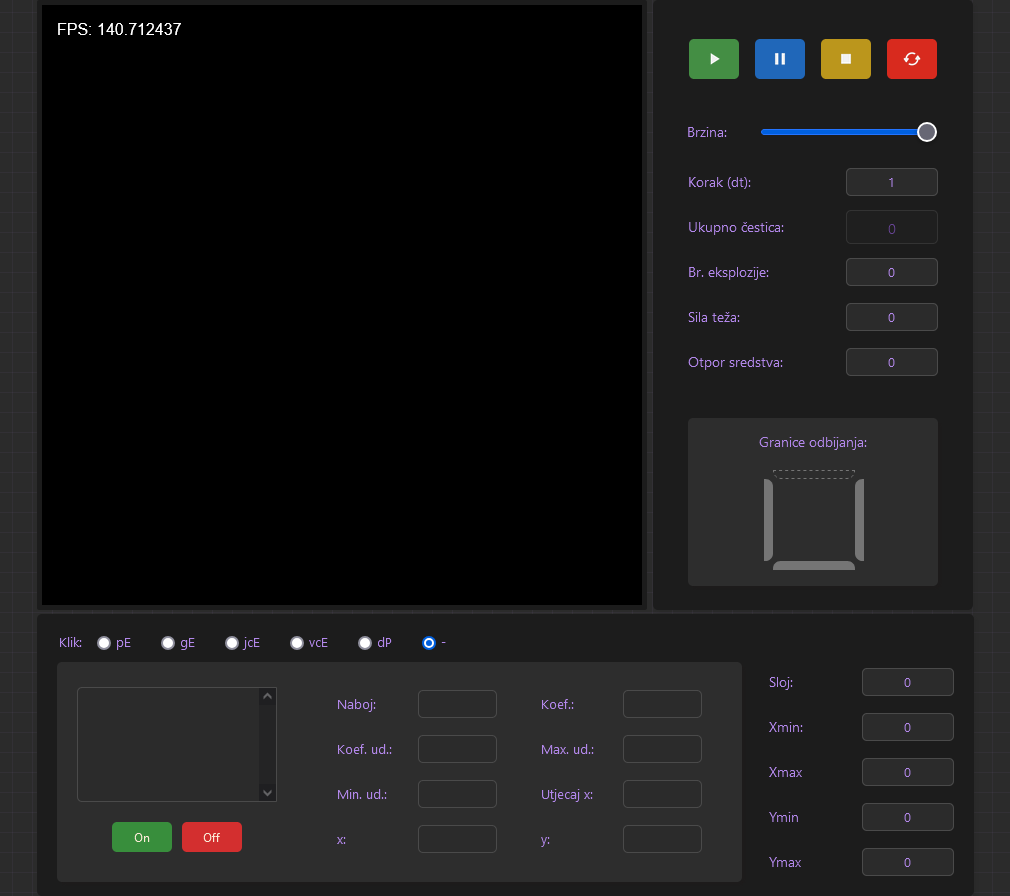
\includegraphics[width=0.9\textwidth]{slike/21_Simulator.png}
    \captionsetup{justification=centering}
    \caption{Višestruka Coulombova eksplozija}
\label{fig:Simulator}
\end{figure}

Simulator se sastoji od crnog platna na kojemu piše trenutni FPS. S desne strane nalaze se obojeni gumbi za pokretanje (plavi), pauziranje (zelen), resetiranje (žuti) i ponovno učitavanje animacije (crveni). Odmah ispod njih, nalazi se \textit{slider} za upravljanje brzinom simulacije i polje za unos u kojemu se može definirati koeficijent preciznosti. Dalje, prikazan je brojač čestica. U njemu je samo prikazan trenutni broj čestica na ekranu i ne može se mijenjati. Parametar \textit{Br. eksplozije} definira koliko čestica će se generirati odabranom eksplozijom, \textit{Sila teža} omogućava promjenu koeficijenta djelovanja sile teže i \textit{Otpor sredstva} omogućava promjenu koeficijenta djelovanja otpora sredstva. Na dnu te desne konzole nalazi se i mogućnost postavljanja granica odbijanja. Također, definirana je dodatna konzola na dnu stranice. Na njoj se može odabrati funkcija koja će se pozivati kada se klikne na platno. To može biti pravilna eksplozija, Gaussova eksplozija, Coulombova eksplozija ili višestruka Coulombova eksplozija. Dalje, na klik se može postaviti i funkcija za postavljanje Coulombovog potencijala na platnu. Na kraju, moguće je postaviti "praznu funkciju", odnosno postaviti funkciju tako da se na klik ne događa ništa. Ispod tih opcija nalazi se prozor u kojemu se nalaze svi definirani potencijali čiji atributi se mogu uređivati unosom vrijednosti u polja. Krajnje desno, nalaze se opcije za postavljanje sloja čestica. Sloj čestica se generira metodom \textit{Math.random()} što znači da naliči kvadratu. 

Ključna klasa za rad simulatora je klasa \textit{Konzola}. Njena inicijalizacija pokreće dohvaćanje svih potrebnih HTML elemenata i njihovo postavljanje, postavljanje vrijednosti unutar klase \textit{Konzola}, praćenje broja čestica, spremanje stanja čestica i potencijala i definiranje svih metoda za rukovanje događajima koji se mogu dogoditi. Svaki put kada se želi postaviti vizualizacija s određenim parametrima, potrebno je definirati HTML datoteku koja poziva skriptu \textit{pokretanje}, definira objekt klase \textit{Parametri} i prosljeđuje ga funkciji \textit{main(parametri)}. Za svaku vrstu eksplozije, definirana je zasebna HTML datoteka, a pokretanjem tih HTML datoteka dobivaju se rezultati na slikama \ref{fig:PESimulator}, \ref{fig:GESimulator}, \ref{fig:CESimulator} i \ref{fig:VCESimulator}.
\begin{figure}[H]
    \centering
    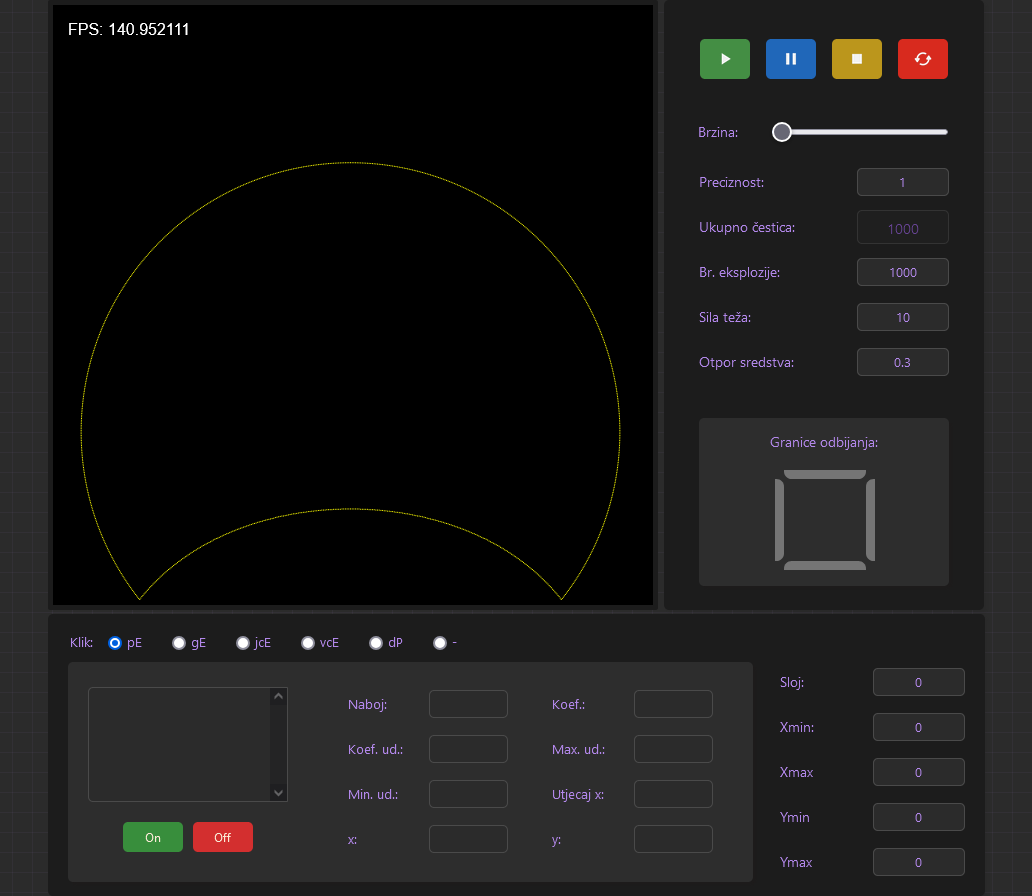
\includegraphics[width=0.9\textwidth]{slike/22_PESimulator.png}
    \captionsetup{justification=centering}
    \caption{Pravilna eksplozija na simulatoru}
\label{fig:PESimulator}
\end{figure}

\begin{figure}[H]
    \centering
    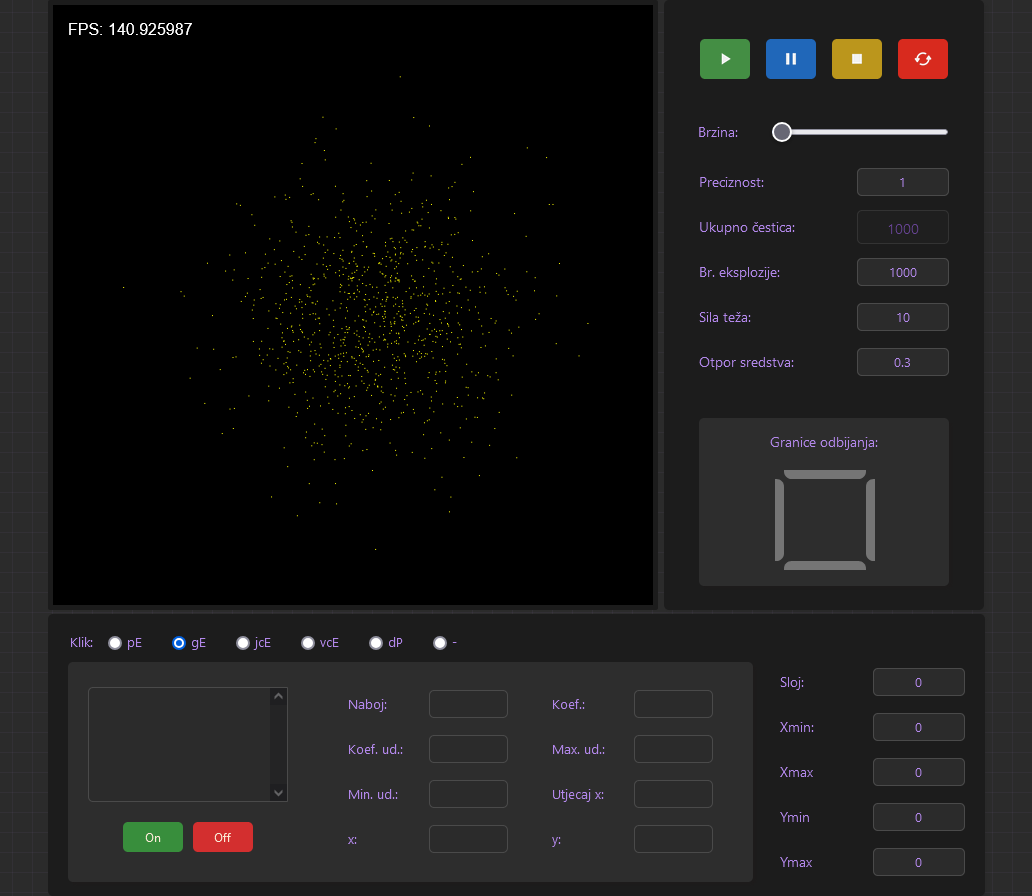
\includegraphics[width=0.9\textwidth]{slike/23_GESimulator.png}
    \captionsetup{justification=centering}
    \caption{Gaussova eksplozija na simulatoru}
\label{fig:GESimulator}
\end{figure}

\begin{figure}[H]
    \centering
    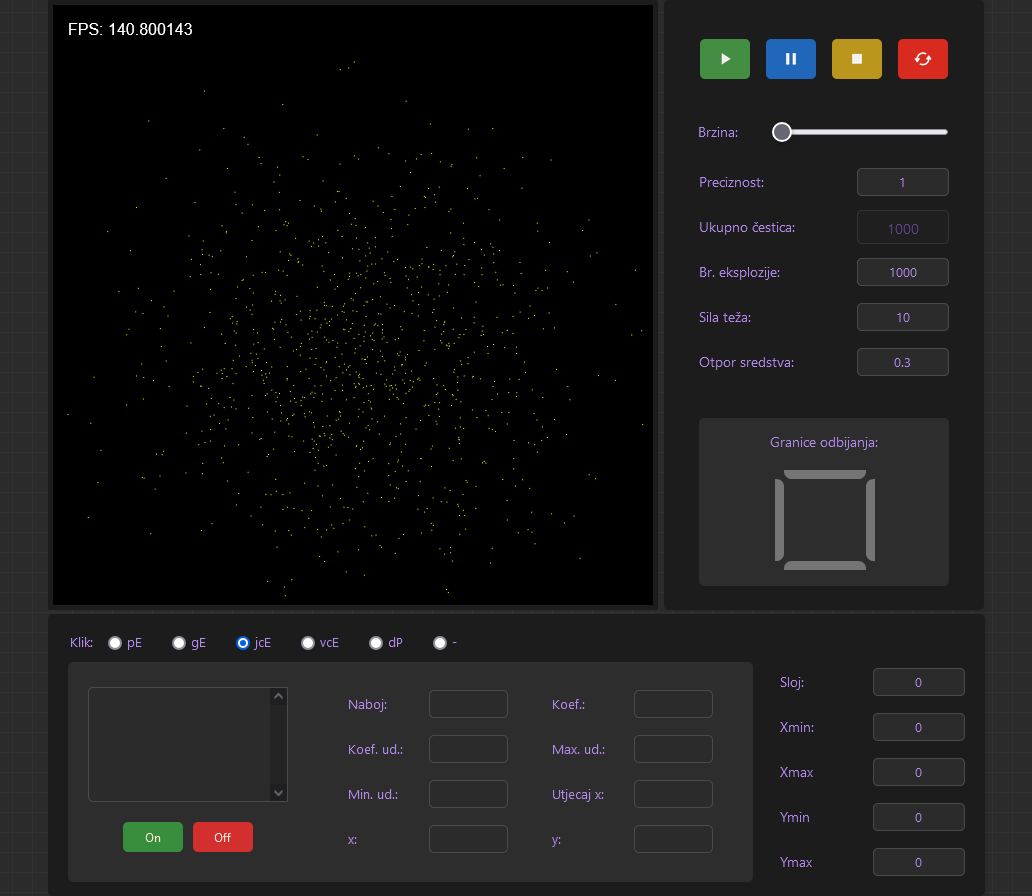
\includegraphics[width=0.9\textwidth]{slike/24_CESimulator.png}
    \captionsetup{justification=centering}
    \caption{Coulombova eksplozija na simulatoru}
\label{fig:CESimulator}
\end{figure}

\begin{figure}[H]
    \centering
    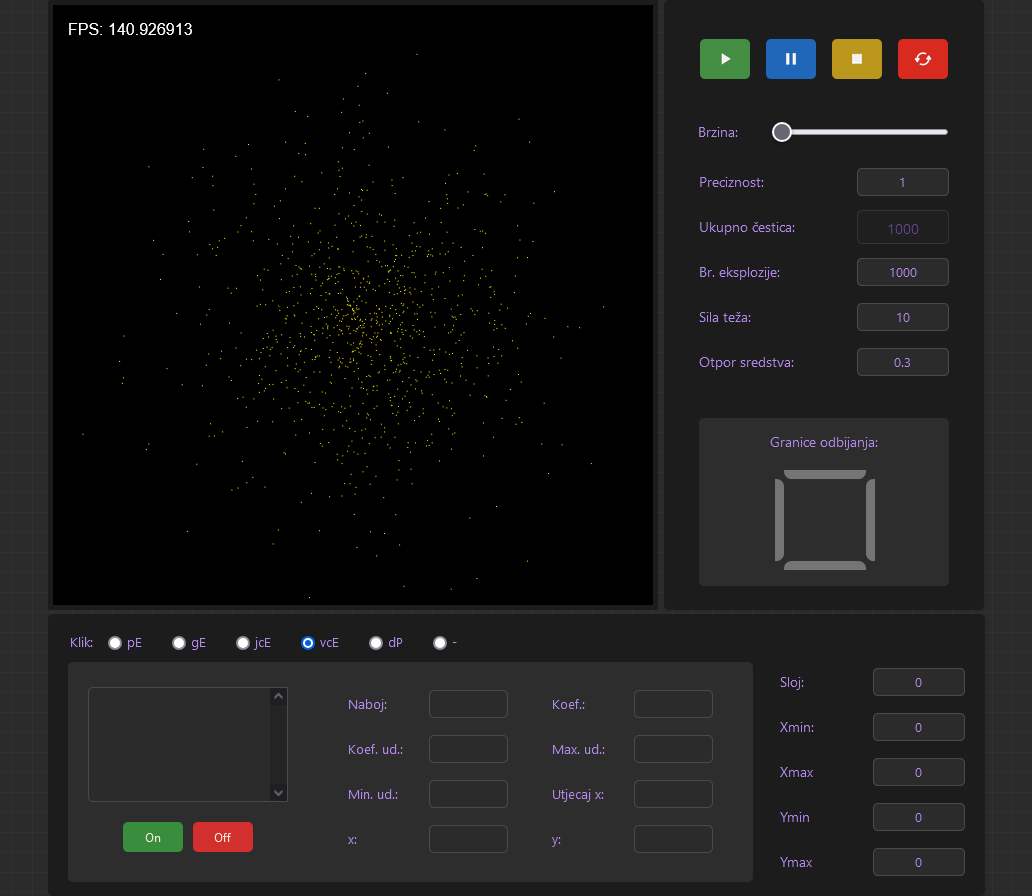
\includegraphics[width=0.9\textwidth]{slike/25_VCESimulator.png}
    \captionsetup{justification=centering}
    \caption{Višestruka Coulombova eksplozija na simulatoru}
\label{fig:VCESimulator}
\end{figure}

Kako bi se prikazale naprednije sposobnosti simulatora, napravljeno je nekoliko vizualizacija u kojima se pokušava prikazati efekt atomske gljive. Za to će se napraviti par različitih HTML datoteka s drugačijim početnim parametrima. Prepoznatljivi oblik gljive nastaje nakon što nuklearna eksplozija stvori prostor ekstremno vrućeg zraka koji se ubrzano diže. Prilikom tog kretanja, zrak se hladi i kreće se širiti prema vrhu čime se stvara "klobuk" gljive. Nakon toga, hladni zrak ispod klobuka se diže prema njemu čime se stvara stručak. Naravno, ova interakcija toplog i hladnog zraka, negativnog tlaka, vakuuma i ostalih faktora je mnogo kompleksnija, no sve te interakcije su ionako prekompleksne za uračunati u ovom simulatoru. Za potrebe prikaza dodatnih sposobnosti simulatora, dovoljno je samo vizualno stvoriti oblik gljive \parencite{MushroomCloudBezDat}.

U prvom pristupu koristit će se nepomični potencijal koji se ugasi nakon što mu se čestice previše približe. Također, definiran je i sloj čestica na dnu koji će predstavljati prašinu koja se diže u oblak. Na slici \ref{fig:NepokretniPotencijal} je prikazan rezultat ove vizualizacije.

\begin{figure}[H]
    \centering
    \includegraphics[width=0.55\textwidth]{slike/26_NepokretniPotencijal.png}
    \captionsetup{justification=centering}
    \caption{Vizualizacija atomske gljive s nepokretnim potencijalom}
\label{fig:NepokretniPotencijal}
\end{figure}

Kako se vidi iz slike \ref{fig:NepokretniPotencijal}, čestice se krenu križati i nakon što se ugasi potencijal gubi se željeni efekt. Iz tog razloga, promijenit će se početni parametri tako da se potencijal pomiče prema gore velikom brzinom i ima smanjen utjecaj na $x$ komponentu vektora pozicije čestica. Rezultat je prikazan na slici \ref{fig:PokretniPotencijal}.

\begin{figure}[H]
    \centering
    \includegraphics[width=0.55\textwidth]{slike/27_PokretniPotencijal.png}
    \captionsetup{justification=centering}
    \caption{Vizualizacija atomske gljive s pokretnim potencijalom}
\label{fig:PokretniPotencijal}
\end{figure}

Ponovo, korištenjem ovih parametara, ne dobiva se željeni izgled gljive. Iz tog razloga, pokušat će se koristiti više potencijala, jedan koji će podignuti sloj čestica i dva koja će raspršiti čestice pri vrhu.  Svi potencijali nestaju nakon što im se čestice previše približe. Rezultat je prikazan na slici \ref{fig:VisePotencijala1}

\begin{figure}[H]
    \centering
    \includegraphics[width=0.55\textwidth]{slike/28_VisePotencijala1.png}
    \captionsetup{justification=centering}
    \caption{Vizualizacija atomske gljive s više nepokretnih potencijala}
\label{fig:VisePotencijala1}
\end{figure}

Ovaj pristup je dovoljno blizu željenom rezultatu, no za dobru mjeru, dodan je još jedan primjer s četiri potencijala. Potencijali su postavljeni kao i u prijašnjem primjeru, no smanjena je udaljenost do koje se čestice smiju približiti kako bi se povećala većina klobuka. Kako se gljiva ne bi raspršila izvan okvira platna i kako bi se bolje raspršio klobuk, dodan je i četvrti potencijal izvan ekrana koji odbija čestice. Rezultat je prikazan na slici \ref{fig:VisePotencijala2}.


\begin{figure}[H]
    \centering
    \includegraphics[width=0.55\textwidth]{slike/29_VisePotencijala2.png}
    \captionsetup{justification=centering}
    \caption{Vizualizacija atomske gljive s više prepravljenih nepokretnih potencijala}
\label{fig:VisePotencijala2}
\end{figure}

Napokon, napravljen je i simulator i odabrana je metoda vizualizacije eksplozije koja će se primijenitit u tri dimenzije. Sljedeći korak je prevođenje predstavljenih koncepata u 3D i primjena \textit{shadera} za simulaciju mnogo većeg broja čestica. Za sada, bilo je moguće prikazati nekoliko desetaka tisuća čestica, no koristeći grafički procesor, cilj je dostići brojku od milijun čestica bez prevelike razlike u performansama vizualizacije.

\chapter{Temeljni koncepti 3D vizualizacije}
Prije izrade 2D vizualizacija, bilo je potrebno napraviti uvodni osvrt na osnovne koncepte računalne grafike na kojima su se one temeljile. Na isti način, prelazak iz dvije u tri dimenzije zahtjeva razumijevanje novih pojmova koji nisu bili potrebni za rad s 2D grafikom.  

\section{Matrični prikaz transformacija}
Osnovni koncept i 2D i 3D grafike su transformacije i njihove matrične reprezentacije. Kako se transformacije nisu previše koristile za vizualizacije 2D eksplozija, nije bilo potrebe za upoznavanje s njima. Sada, matrične transformacije čine osnovu za prelazak u višu dimenziju.

Osnovne transformacije koje se mogu vršiti nad 2D objektima su translacija, skaliranje i rotacija. Prva transformacija, translacija, može se intuitivno izvesti. Recimo da je definirana točka $A$ s koordinatama $(2, 1)$. Točku $A$ potrebno je pomaknuti na poziciju $(-1, 5)$. Kako bi se znala izvršiti translacija, potrebno je pronaći varijable $x$ i $y$ koje će se dodati točki $A$ kako bi se ona nalazila na željenoj poziciji. Očito, dovoljno je oduzeti koordinate željene pozicije od trenutno pozicije točke $A$. Odnosno, $x$ će biti -3, a $y$ će biti 4. Zasada, matrični zapis ove transformacije može izgledati kao zbrajanje dvaju vektora, odnosno dviju matrica:
\[
\begin{bmatrix}
x'\\
y' 
\end{bmatrix}
=
\begin{bmatrix}
x\\
y
\end{bmatrix}
+
\begin{bmatrix}
a_x\\
a_y
\end{bmatrix}
\]
Bitno je za napomenuti da ovakav prikaz translacije nije praktičan, ali tek kasnije će se objasniti zašto. Translacija točke prikazana je na slici \ref{fig:Translacija}. Vektori $a_x$ i $a_y$ na slici predstavljaju pomake po $x$ i $y$ osi. Plava točka predstavlja točku koji je potrebno translatirati, a crvena točka predstavlja točku nakon translacije. Translacija objekta je ista kao i translacija točke, no umjesto jedne točke, translatiraju se sve točke objekta. 

\begin{figure}[H]
    \centering
    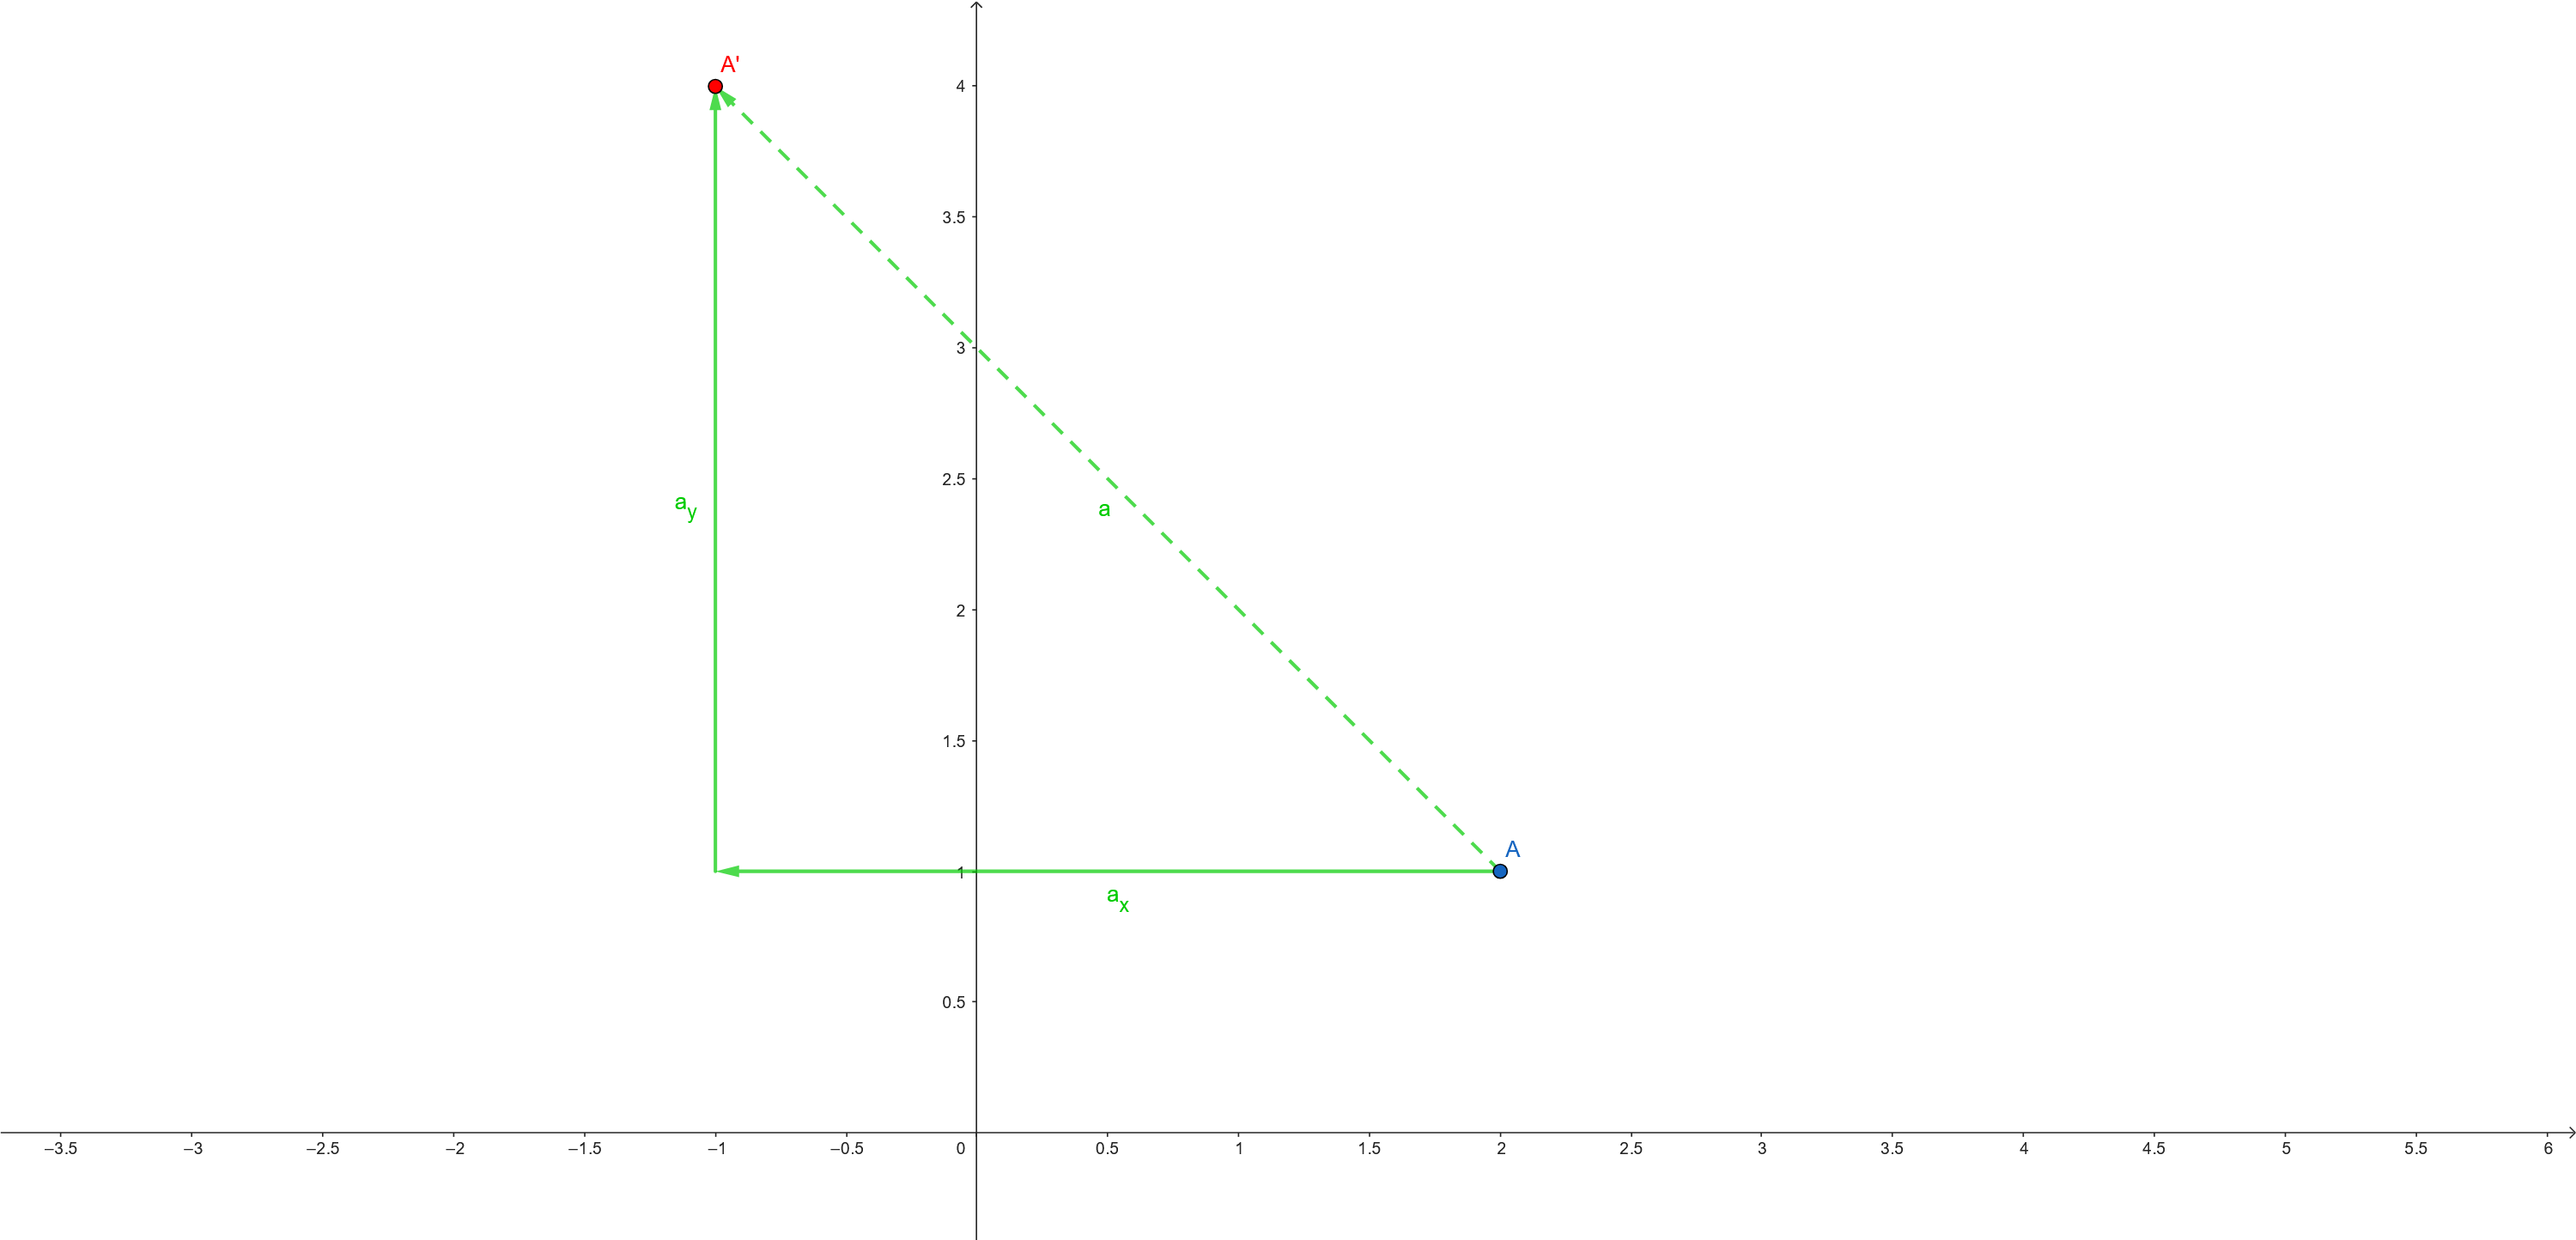
\includegraphics[width=0.95\textwidth,trim={2cm 0cm 3cm 0cm},clip]{slike/30_Translacija.png}
    \captionsetup{justification=centering}
    \caption{Translacija točke $A$ u točku $A'$}
\label{fig:Translacija}
\end{figure}

Dalje, operacija skaliranja se odnosi na promjenu veličine objekta. Umjesto zbrajanja matrica kao što je to bilo prikazano u primjeru za translaciju, ovdje je potrebno množiti matrice. Množenje je potrebno jer se operacija skaliranja svodi na pomicanje točaka objekta $s$ puta u nekom smjeru. Tako se dobiva efekt povećavanja i smanjivanja objekta. Na primjer, ako je potrebno trostruko povećati dužinu $\overline{AB}$, definiranu točkama $A = (1, 1)$ i $B = (2, 2)$, dovoljno je pomnožiti njene točke skalarom čija je vrijednost 3. Ova transformacija je prikazana na slici \ref{fig:Skaliranje}. Plava dužina predstavlja početnu dužinu $\overline{AB}$, a crvena dužina predstavlja skaliranu dužinu. Matrični prikaz ove transformacije naveden je ispod:
\[
\begin{bmatrix}
x'\\
y' 
\end{bmatrix}
=
\begin{bmatrix}
s_x & 0\\
0 & s_y
\end{bmatrix}
\begin{bmatrix}
x\\
y
\end{bmatrix}
\]


\begin{figure}[H]
    \centering
    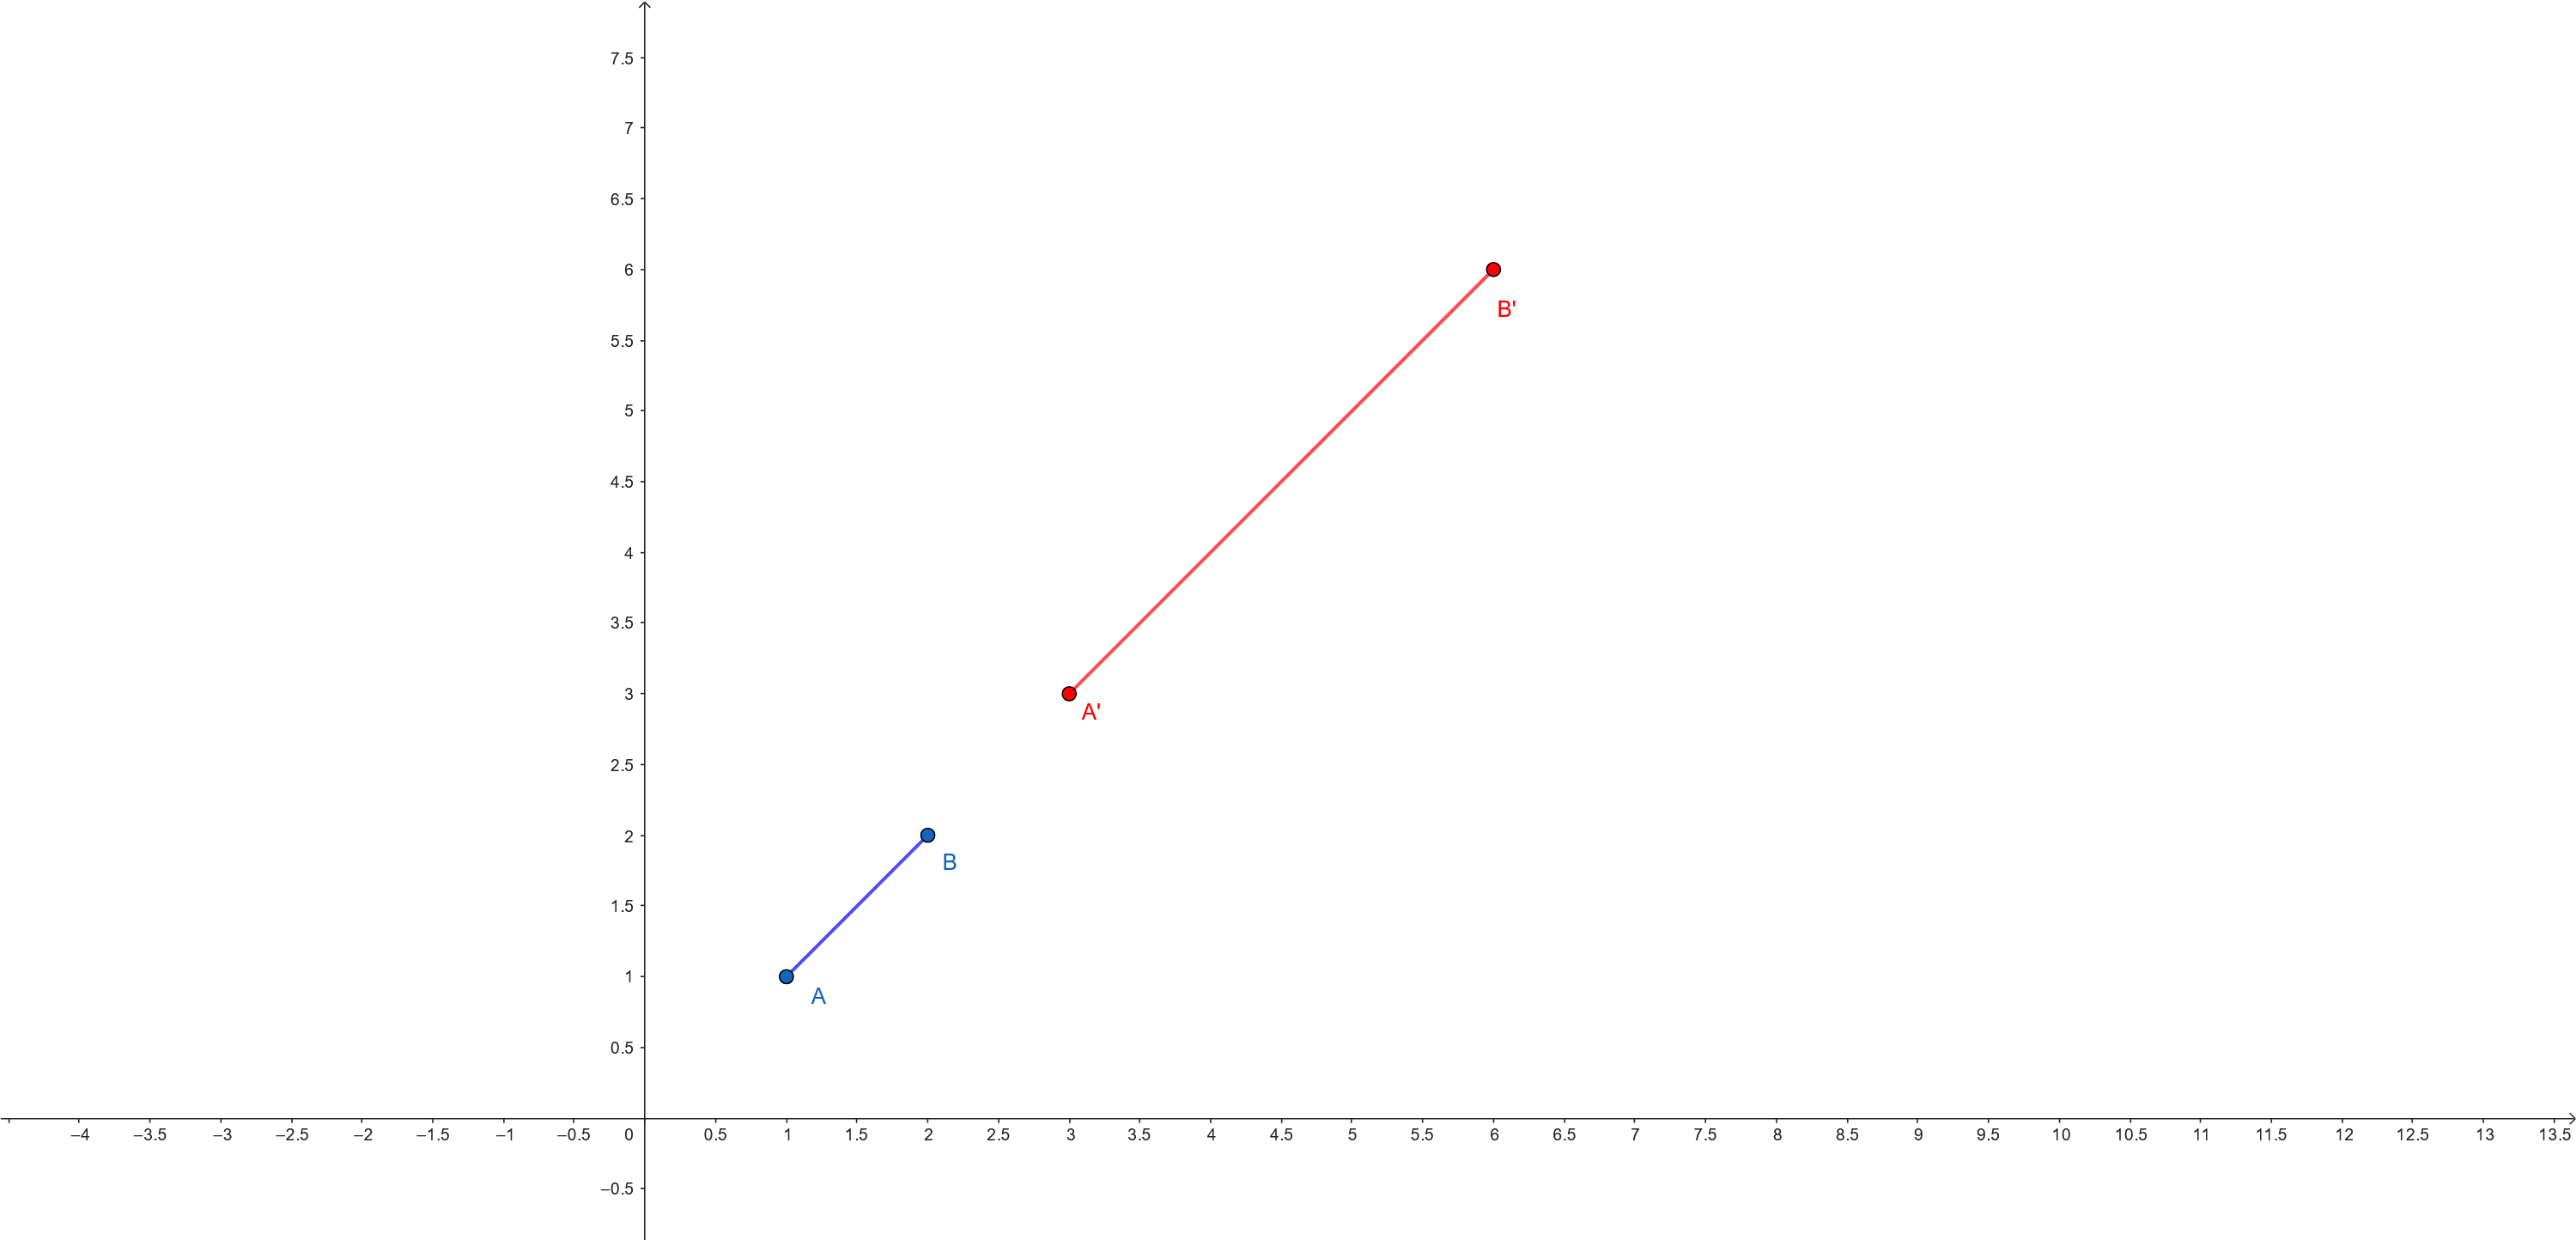
\includegraphics[width=1\textwidth,trim={3cm 0cm 3cm 0cm},clip]{slike/31_Skaliranje.png}
    \captionsetup{justification=centering}
    \caption{Skaliranje dužine $\overline{AB}$}
\label{fig:Skaliranje}
\end{figure}




Sljedeća transformacija koristi složenije funkcije za izvođenje. Temelj rotacije je pomicanje točaka po kružnici koja se nalazi u središtu koordinatnog sustava. Koristeći trigonometrijske funkcije, ova transformacija se može zapisati kao:

\[
\begin{bmatrix}
x'\\
y' 
\end{bmatrix}
=
\begin{bmatrix}
cos(\theta) & -sin(\theta)\\
sin(\theta) & cos(\theta)\\
\end{bmatrix}
\begin{bmatrix}
x\\
y
\end{bmatrix}
=
\begin{bmatrix}
xcos(\theta)-ysin(\theta)\\
xsin(\theta)+ycos(\theta)\\
\end{bmatrix}
\]

Slika \ref{fig:Rotacija} prikazuje dužinu $\overline{AB}$ iz prijašnjeg primjera. Ona je obojena plavo. Druga dužina $\overline{A'B'}$ zelene boje predstavlja dužinu $\overline{AB}$ koja je rotirana za $45^{\circ}$. Crne iscrtane kružnice predstavljaju kružnice po kojima se početna i završna točka kreću tijekom rotacije. Rotiranje ove dužine za bilo koji kut će rezultirati dužinom čija se početna i završna točka nalaze na nacrtanim kružnicama \parencite{2DTransform}. 

\begin{figure}[H]
	\centering
	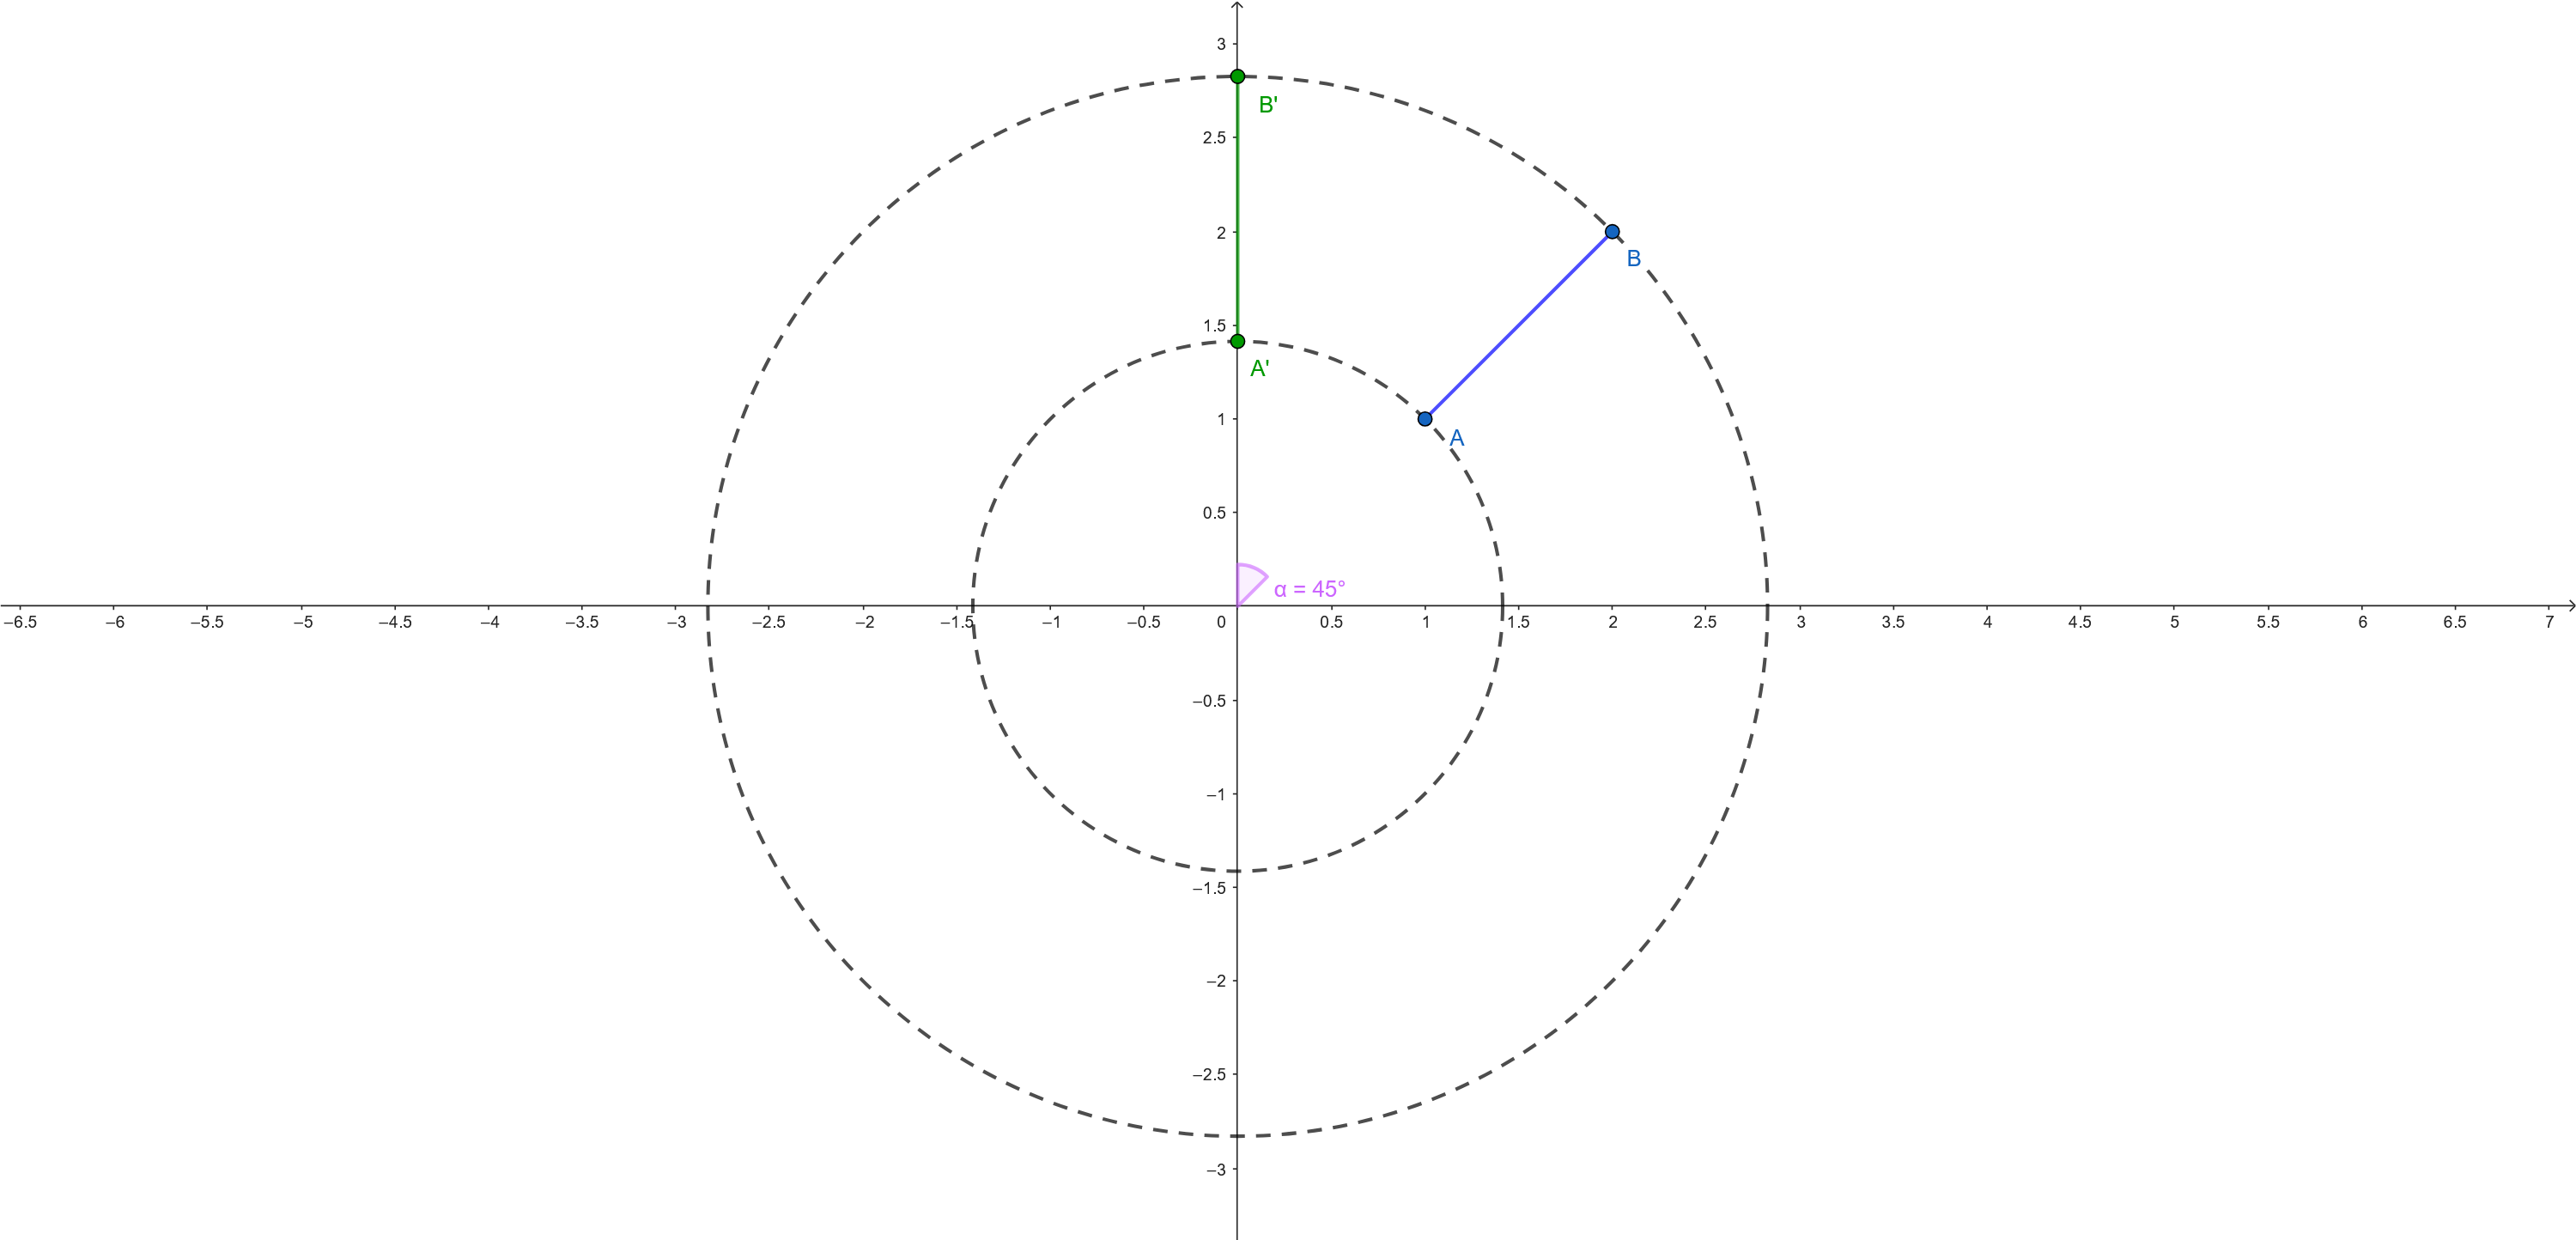
\includegraphics[width=1\textwidth,trim={3cm 0cm 3cm 0cm},clip]{slike/32_Rotiranje.png}
	\captionsetup{justification=centering}
	\caption{Rotiranje dužine $\overline{AB}$}
	\label{fig:Rotacija}
\end{figure}

Nekada pojedinačne operacije nisu dovoljne. Ako se želi napraviti program u kojemu se dužine mogu pomicati i razvlačiti mišem pootrebno je implementirati \textit{drag'n'drop} operacije nad dužinama. Ako korisnik mišem klikne na dužinu, može ju "nositi" mišem po ekranu. Očito, koristit će se translacija. Dalje, korisnik želi produljiti dužinu tako da ju povuče za jednu krajnju točku. Ovdje je očito da se treba koristiti skaliranje, no na slici \ref{fig:Skaliranje} operacija skaliranja skalira i pomiče cijelu dužinu. Kada bi korisnik povukao dužinu mišem  koristeći samo skaliranje, ona bi se povećala i micala u smjeru u kojemu se skalira. Još gore, ako korisnik odluči povući dužinu lijevo ili desno, dužina će se odjednom rotirati oko ishodišta koordinatnog sustava. Rješenje ovog problema nalazi se baš u ishodištu koordinatnog sustava. Ako se pokuša skalirati ili rotirati dužina čija se krajnja točka nalazi u ishodištu, dužina će ostati "usidrena" u ishodištu. Iz tog razloga, dužinu je potrebno prvo translatirati, zatim skalirati i rotirati. Na kraju, potrebno je translatirati dužinu za isti negativni vektor. Slike \ref{fig:TransSkalRot} i \ref{fig:TransSkalRotKraj} prikazuju ove transformacije. Slika \ref{fig:TransSkalRot} čitana s lijeva na desno prikazuje početnu dužinu (crna), početnu dužinu translatiranu u ishodište (žuta), skaliranu translatiranu dužinu (crvena) i rotiranu skaliranu dužinu (ljubičasta). Nakon svih izvršenih transformacija, dužina se još uvijek nalazi u ishodištu. Jedino što je preostalo je vratiti ju na početnu poziciju. Na slici \ref{fig:TransSkalRotKraj} zelena dužina predstavlja rezultat nakon završne translacije, a crna dužina predstavlja početnu dužinu $\overline{AB}$. 


\begin{figure}[H]
	\centering
	\includegraphics[width=1\textwidth]{slike/33_TransSkalRot.png}
	\captionsetup{justification=centering}
	\caption{Rotiranje dužine $\overline{AB}$}
	\label{fig:TransSkalRot}
\end{figure}
\begin{figure}[H]
	\centering
	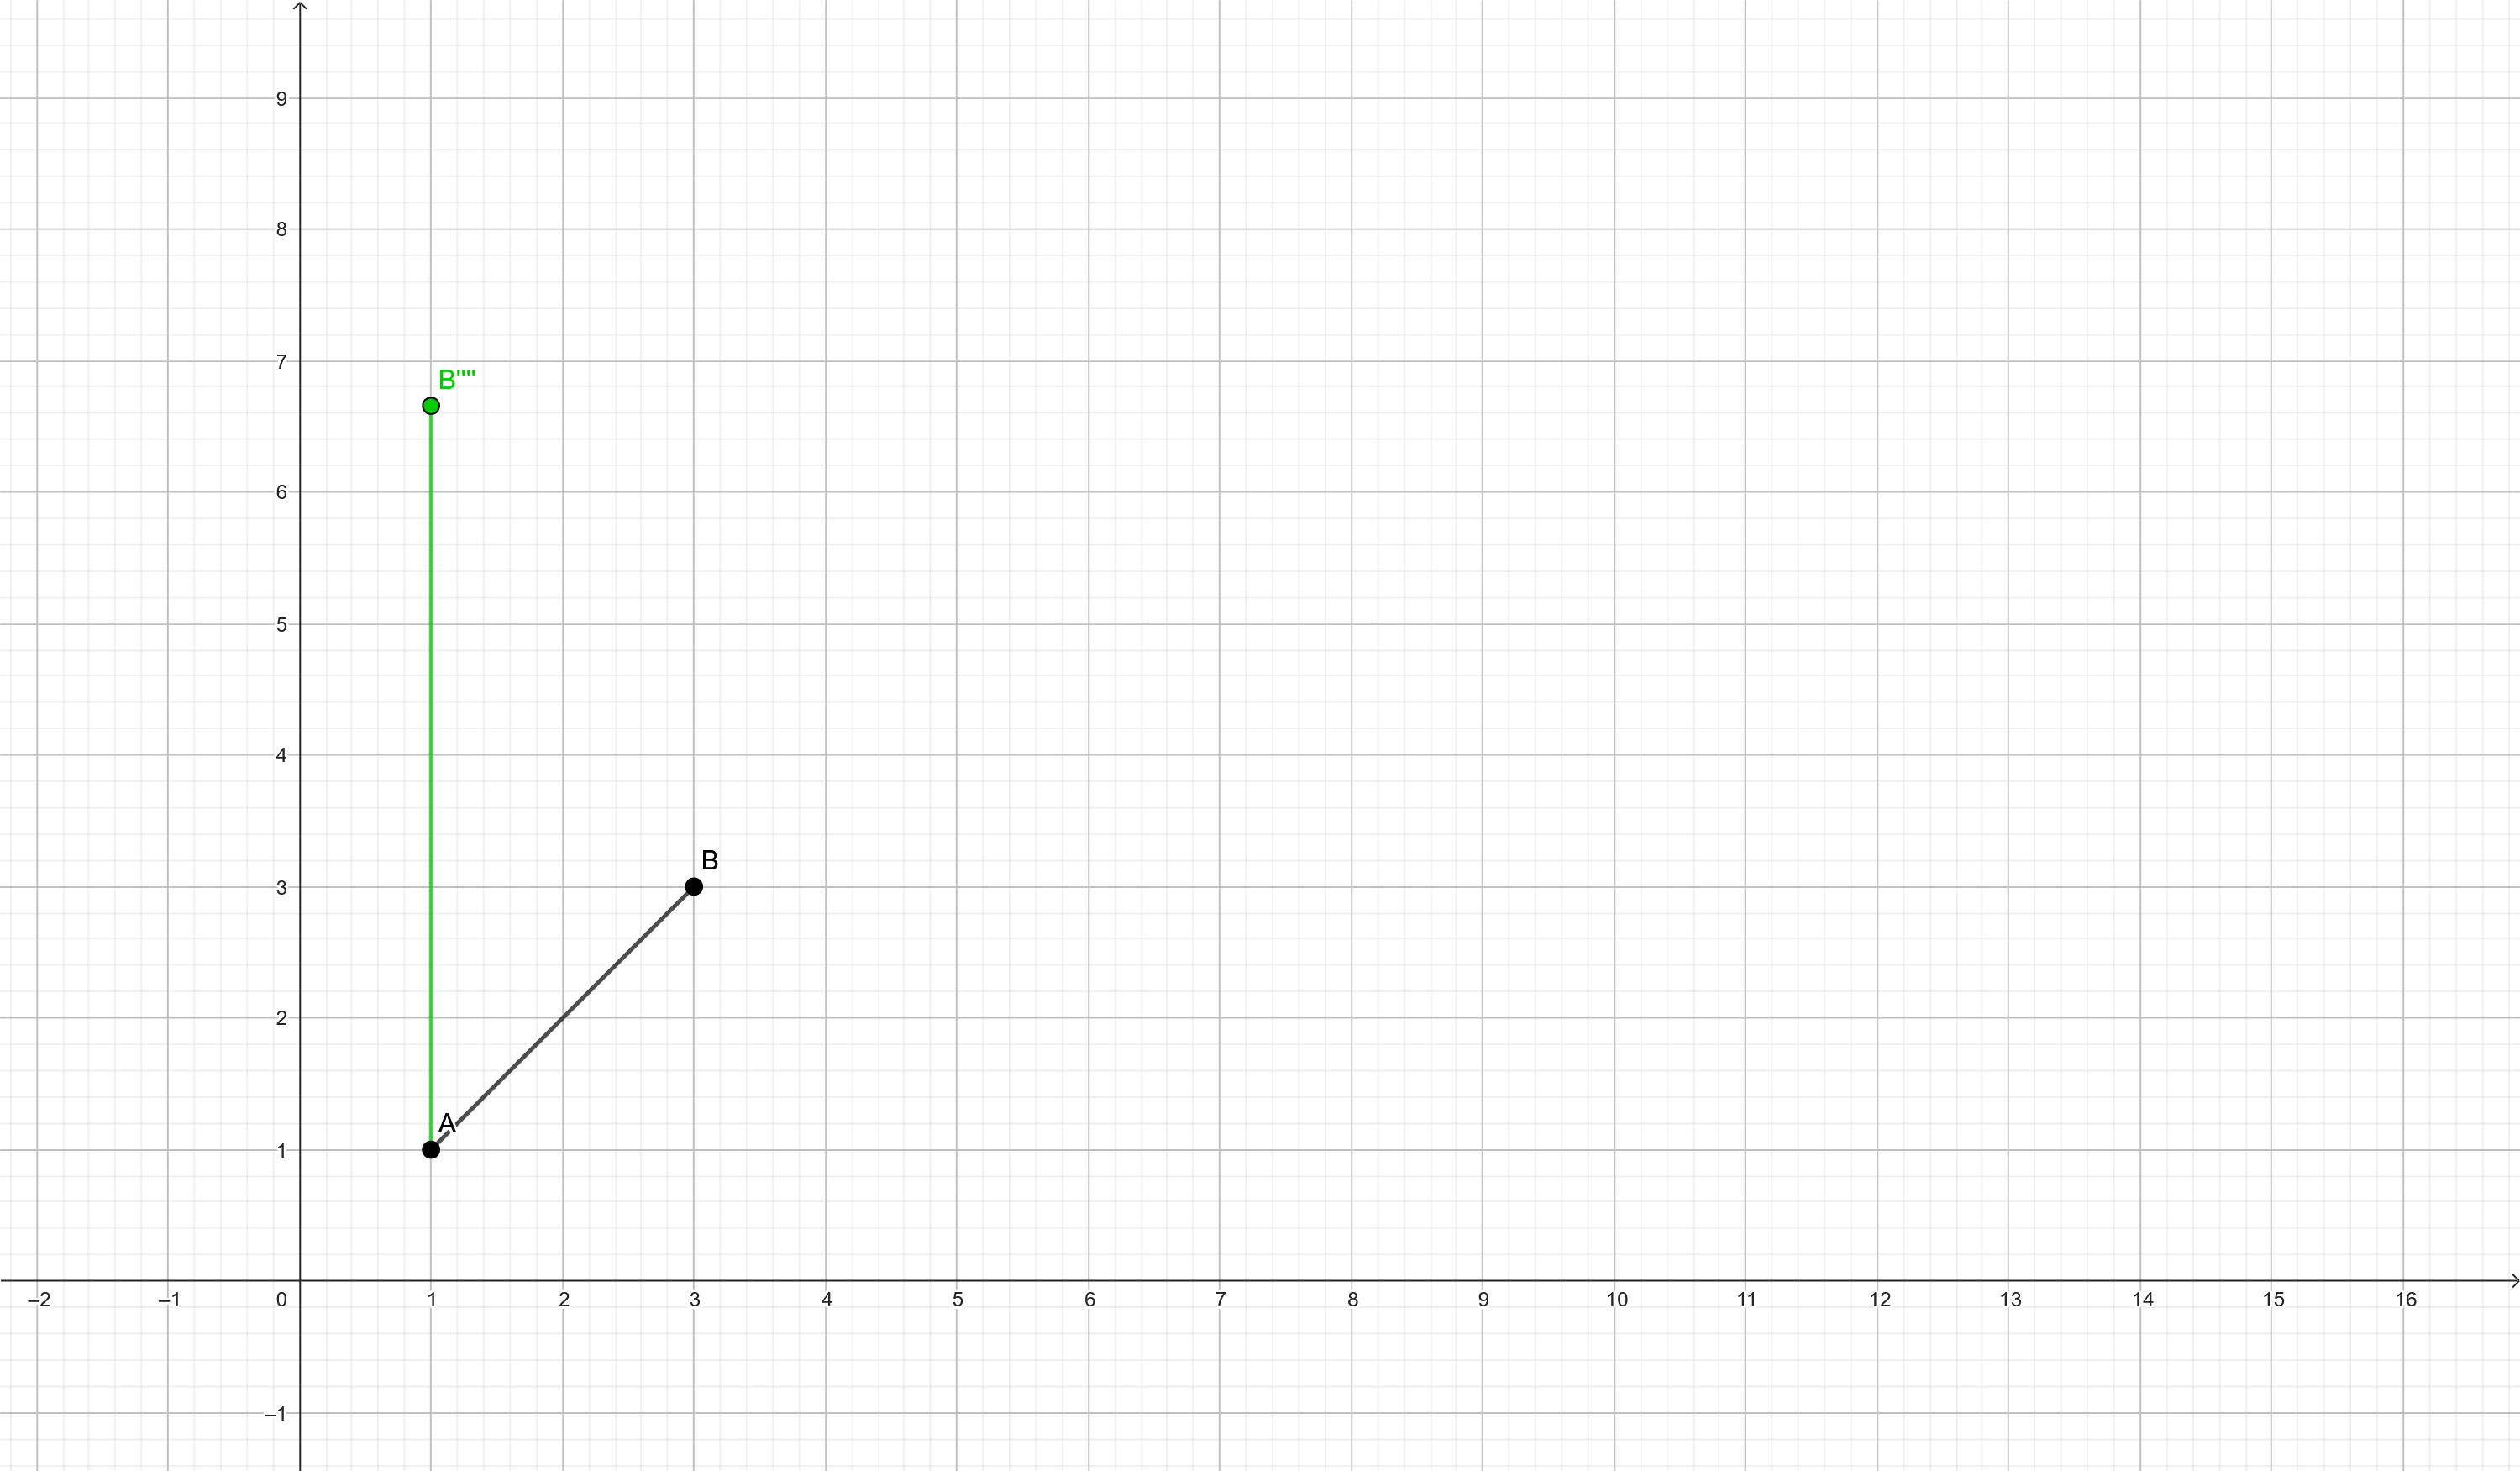
\includegraphics[width=1\textwidth]{slike/34_TransSkalRotKRAJ.png}
	\captionsetup{justification=centering}
	\caption{Rotiranje dužine $\overline{AB}$}
	\label{fig:TransSkalRotKraj}
\end{figure}

Ove transformacije se mogu izvesti tako da se prvo provede translacija, zatim skaliranje, rotacija i na kraju završna translacija. Sada je najpraktičnije koristi matrični zapis transformacija. Zbog svojstava matrica, moguće je množiti svaku matricu transformacije jednu s drugom u suprotnom redu od onog u kojemu ih je potrebno izvršavati. Tako se dobiva jedna matrica transformacije koja predstavlja novu transformaciju, ona u kojoj se dužina rotira i skalira oko svoje početne točke $A$. Potrebno je napomenuti kako se redoslijed množenja matrica ne može mijenjati jer operacija množenja matrica nije komutativna. Odnosno, ako su $A_{ij}$ i $B_{ij}$ matrice, tada:

\begin{align*}
A_{ij}B_{ij}\neq B_{ij}A_{ij}.
\end{align*}

Dalje, nekada je potrebno izvršiti suprotnu operaciju, u ovom slučaju translaciju. Nakon postavljanja dužine u ishodište i izvršavanja svih transformacija, treba vratiti dužinu na njenu početnu poziciju. Odnosno, nakon translacije $T(A)$ gdje $T$ predstavlja samu operaciju, a $A$ predstavlja točku pomaka, izvršava se operacija $T(A)^{-1}$. Dakle, matrice olakšavaju izvođenje suprotne (inverzne) operacije računanjem inverza matrice transformacije. Operacija rotiranja i skaliranja dužine oko njene početne točke može se zapisati kao:

\begin{align*}
T(a_x,a_y)R(\theta)S(s_x,s_y)T(a_x,a_y)^{-1}
\end{align*}\\
gdje su $T$,$R$ i $S$ translacija, rotiranje i skaliranje, a $(a_x, a_y)$, $\theta$ i $(s_x, s_y)$ su pomak translacije, kut rotacije i faktori skaliranja. Matrice transformacije se množe suprotnim redom od transformacija koje se trebaju izvesti. Iz tog razloga, prvo se množi matrica rotacije s matricom skaliranja. 

Trenutno, matrice nisu u pravilnom obliku za međusobno množenje. Nije moguće pomnožiti matricu translacije s matricom rotacije ili skaliranja. Iz tog razloga, potrebno je sve matrice modificirati kako bi se mogle međusobno množiti. Prvo je potrebno promijeniti matricu translacije. Ako se radi o dvodimenzionalnoj translaciji, nije moguće napraviti kvadratnu matricu drugog reda, odnosno matricu s dva reda i dva stupca. Iz tog razloga, matrici se dodaje još jedan stupac i redak, a vektoru nad kojim se vrši transformacija se dodaje još jedna koordinata:

\[
\begin{bmatrix}
	1 & 0 & a_x\\
	0 & 1 & a_y\\
	0 & 0 & 1
\end{bmatrix}
\]

Ovakav zapis koristi homogene koordinate. Homogene koordinate opisuju točku u prostoru čiji se članovi dijele s posljednjim članom kako bi se dobila prave koordinate. Na primjer, homogene koordinate (6,1,3) se mogu predstaviti i kao (2,$\frac{1}{3}, 1$). Homogene koordinate omogućavaju korištenje raznih transformacija na jednostavniji način. Dalje, sve matrice transformacija se pretvaraju u kvadratne matrice trećeg reda kako bi se mogle množiti. Time je matrica skaliranja predstavljena ovako:

\[
\begin{bmatrix}
	s_x & 0 & 0\\
	0 & s_y & 0\\
	0 & 0 & 1
\end{bmatrix}
\]
\\Dalje, matrica rotacije je predstavljena ovako:

\[
\begin{bmatrix}
	cos(\theta) & -sin(\theta) & 0\\
	sin(\theta) & cos(\theta) & 0\\
	0 & 0 & 1
\end{bmatrix}.
\]
\\Na kraju, operacija skaliranja i rotacije dužine oko početne točke se može predstaviti sljedećim umnoškom matrica:

\[
\begin{bmatrix}
	1 & 0 & a_x\\
	0 & 1 & a_y\\
	0 & 0 & 1
\end{bmatrix}
\begin{bmatrix}
	cos(\theta) & -sin(\theta) & 0\\
	sin(\theta) & cos(\theta) & 0\\
	0 & 0 & 1
\end{bmatrix}
\begin{bmatrix}
	s_x & 0 & 0\\
	0 & s_y & 0\\
	0 & 0 & 1
\end{bmatrix}
\begin{bmatrix}
1 & 0 & a_x\\
0 & 1 & a_y\\
0 & 0 & 1
\end{bmatrix}^{-1}.
\]

Primjenom ove matrice transformacije nad svim točkama dužine, dobiti će se željeni rezultat. Naravno, postoji još nekoliko transformacija koje se često izvode, no zasada ih nije potrebno navoditi. Matrice transformacije se lako prenose u tri dimenzije. Kao i u dvije dimenzije, matrice moraju imati dodatan redak i stupac jer koriste homogene koordinate. Tako će sve matrice transformacije za tri dimenzije biti kvadratne matrice četvrtog reda. Matrice su vrlo slične dvodimenzionalnim verzijama. Matrica translacije izgleda ovako:
\[
\begin{bmatrix}
	1 & 0 & 0 & a_x\\
	0 & 1 & 0 & a_y\\
	0 & 0 & 1 & a_z\\
	0 & 0 & 0 & 1\\
\end{bmatrix}
\].
\\Ponovo, matrica skaliranja nalikuje svojoj dvodimenzionalnoj verziji:
\[
\begin{bmatrix}
	s_x & 0 & 0 & 0\\
	0 & s_y & 0 & 0\\
	0 & 0 & s_z & 0\\
	0 & 0 & 0 & 1
\end{bmatrix}
\]
\\Matrica rotacije zapravo ne postoji u toliko sličnom obliku u tri dimenzije. To je zato što u tri dimenzije ne postoji jedinstvena rotacija, odnosno objekt se može rotirati oko svake od tri osi prostora. Matrica rotacije oko osi $z$ glasi:

\[
\begin{bmatrix}
	cos(\theta) & -sin(\theta) & 0 & 0\\
	sin(\theta) & cos(\theta) & 0 & 0\\
	0 & 0 & 1 & 0\\
	0 & 0 & 0 & 1
\end{bmatrix}
\]
\\Matrica oko osi $x$ glasi:

\[
\begin{bmatrix}
	1 & 0 & 0 & 0\\
	0 & cos(\theta) & -sin(\theta) & 0\\
	0 & sin(\theta) & cos(\theta) & 0\\
	0 & 0 & 0 & 1
\end{bmatrix}
\]
\\Na kraju, matrica rotacije oko osi $y$ izgleda ovako:

\[
\begin{bmatrix}
	cos(\theta) & 0 & sin(\theta) & 0\\
	0 & 1 & 0 & 0\\
	-sin(\theta) & 0 & cos(\theta) & 0\\
	0 & 0 & 0 & 1
\end{bmatrix}
\]
\\Matrice transformacija su ključne za sve vizualizacije, a pogotovo one koje se odvijaju u tri dimenzije. Ne samo to, već su baš one ključne za prijelaz iz dvije u tri dimenzije \parencite{TransformationMatricesBezDat}.

\section{Ortogonalna i perspektivna projekcija}
Prelazak u tri dimenzije koristi mnogo više transformacija nego što je to bilo potrebno za dvije dimenzije. U dvije dimenzije prelazilo se iz lokalnih koordinata u globalne i na kraju iz globalnih u koordinate ekrana. Ovdje je zapravo bilo potrebno napraviti samo jednu eksplicitnu transformaciju, iz globalnih koordinata u koordinate ekrana. Za to je napravljena posebna klasa \textit{GlobalniKoordinatniSustav}. Umjesto korištenja termina "koordinate", može se govoriti o prostorima kao što su lokalni prostor, globalni prostor i prostor zaslona, odnosno \textit{screen space}. Tako je objekt definiran u lokalnom prostoru definiran svojim lokalnim koordinatama, objekt u globalnom prostoru ima globalne koordinate i tako dalje. U tri dimenzije, potrebno je "proći" kroz šest prostora: lokalni, globalni, prostor pogleda (\textit{view space}), odsječni prostor (\textit{clip space}), normalizirane koordinate uređaja (\textit{Normalized Device Coordinates} ili NDC) i već spomenuti prostor zaslona.

Lokalni prostor se odnosi na prostor u kojemu neki objekt "počinje", odnosno prostor na temelju kojeg se neki osnovni objekt definira. Globalni prostor se odnosi na prostor u kojemu se nalazi više različitih objekata koji su definirani u odnosu jedni na druge. Oni su sačinjeni od transformiranih objekata iz lokalnog prostora. Prostor zaslona odnosi se na prostor definiran zaslonom na kojemu se svi objekti prikazuju. Ovi prostori su vezani uz pojmove lokalnih, globalnih i zaslonskih koordinata, a trenutno je potrebno posvetiti više pažnje prostoru pogleda i \textit{clip} prostoru, ali i NDC-u.  

Prostor pogleda se još naziva i \textit{view space}. Objekti se transformiraju u ovaj prostor izvršavanjem raznih transformacija. Rezultat je pogled na prostor kao iz kamere koja gleda na njega. Na ekranu bi se tada vidio prostor koji kao da se gleda kroz kameru ili iz perspektive nekog promatrača. Transformacije potrebne za dobivanje ovakvog prostora se spremaju u tzv. \textit{view} matricu ili matricu pogleda. 

Dalje, \textit{clip} prostor se odnosi na prostor u kojemu su neke točke odbačene zbog definiranog kriterija. Kriterij se temelji na određivanju raspona vrijednosti i ako koordinate točke nisu u tome rasponu, ona se ne prikazuje. Prvo je potrebno napraviti matricu projekcije koja će pretvoriti koordinate iz prostora pogleda u \textit{clip} prostor. Ovdje se zapravo sve 3D točke projiciraju na 2D "ekran" i na neki način se stvara "iluzija" trodimenzionalnosti. Ova matrica projekcije definira prostor koji se vidi. Sve točke koje se nalaze u tom prostoru su vidljive na ekranu. Prostor koji će biti vidljiv se još naziva i frustum. Frustum je dio piramide koji ostaje nakon što mu se ukloni vrh (manja piramida) koji se nalazi iznad ravnine koja sječe piramidu, a paralelna je s bazom piramide. Prikaz frustuma za perspektivnu projekciju nalazi se na slici \ref{fig:FrustumPerpspektivneProjekcije}. On je obojen plavom bojom i ograničen dvjema ravninama, zelenom i ljubičastom. O ovom prikazu više kasnije. Frustum za ortogonalnu projekciju je samo kuboid, na primjer kocka.


\begin{figure}[H]
	\centering	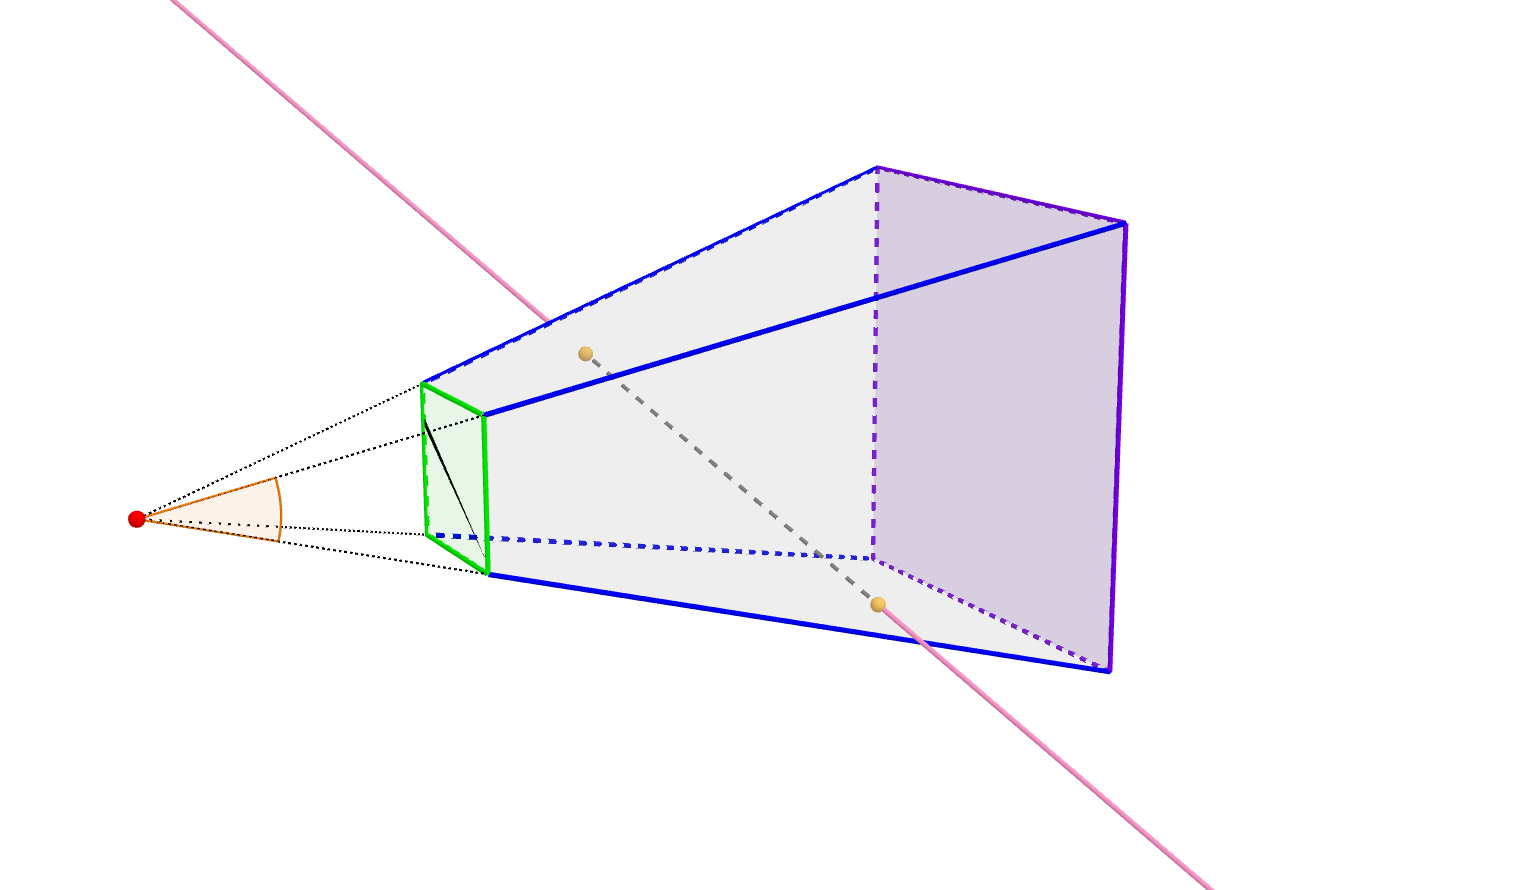
\includegraphics[width=0.95\textwidth,trim={4cm 0cm 10cm 0cm},clip]{slike/35_FrustumPerspektivneProjekcije.png}
	\captionsetup{justification=centering}
	\caption{Frustum perspektivne projekcije}
	\label{fig:FrustumPerpspektivneProjekcije}
\end{figure}

Zadnji korak prije računanja zaslonskih koordinata je pretvorba \textit{clip} prostora u NDC. NDC je prostor koji je ograničen vrijednostima od -1 do 1. Transformacija iz \textit{clip} prostora u NDC se temelji na prelasku iz trenutnih koordinata točke u homogene koordinate. Kako je rečeno u prijašnjem potpoglavlju, svaka točka u prostoru će imati jednu više komponentu nego dimenzija u prostoru. Tako bi u dvije dimenzije točka bila prikazana kao vektor $[x, y, 1]$. U tri dimenzije, koristi se vektor $[x, y, z, w]$, a kako bi se dobile homogene koordinate, potrebno je cijeli vektor podijeliti sa skalarom $w$. Tada su homogene koordinate $[\frac{x}{w},\frac {y}{w}, \frac{z}{w}, 1]$. To dijeljenje skalarom $w$ predstavlja pretvorbu iz \textit{clip} prostora u NDC. Ovo je prostor u koji grafički procesor automatski postavlja sve točke nakon što ih dobije i treba ih nacrtati \parencite{Prostori3DBezDat}. 


Nakon pojašnjenja svih prostora, potrebno je ponovno posjetiti matricu projekcije. Ona može definirati dvije transformacije: ortogonalnu i perspektivnu projekciju. Ortogonalna projekcija ima jednostavan frustum koji izgleda kao "kutija", odnosno frustum je kuboid. Glavni parametri potrebni za stvaranje ortogonalne projekcije su visina, širina i dužina frustuma. Njima se definira frustum i njegova bliska i daleka ravnina. Bliska i daleka ravnina određuju od kud do kud se vide objekti. Dalje, matrica projekcije normalizira sve koordinate unutar frustuma u normalizirane koordinate uređaja tako da su svi objekti prikazani u 3D-u odmah nakon množenja s matricom projekcije. Ortogonalna projekcija se zapravo sastoji od samo 3 operacije: translacije objekta u ishodište, skaliranje objekta kako bi stao u frustum i preokretanje po $z$ osi. Translacija i skaliranje imaju smisla jer se objekti pokušavaju smjestiti u frustum određene veličine. Preokretanje $z$ osi se mora desiti jer je ona preokrenuta u \textit{clip} prostoru što je samo stvar konvencije. Ortogonalna projekcija omogućava prikaz u tri dimenzije, no ona ne daje najrealističniji rezultat. Do toga dolazi jer se ortogonalnom projekcijom ne uračunava i $z$ komponenta i kako ona utječe na veličinu objekta, odnosno, ne uračunava se perspektiva. Svi objekti koji su iste veličine ostaju iste veličine bez obzira na to koliko su udaljeni od promatrača. Iako ovakav način projiciranja ima neke benefite, za potrebe vizualizacije čestica potrebno je uračunati i perspektivu. Prikaz dviju kocki koje su dobivene korištenjem ortogonalne projekcije nalazi se na slici \ref{fig:OrtogonalnaProjekcijaKuba}. Kao što se vidi iz slike, iako su kocke postavljene tako da je jedna ispred druge, one su jednake veličine \parencite{Orto3DBezDat}.

\begin{figure}[H]
	\centering
	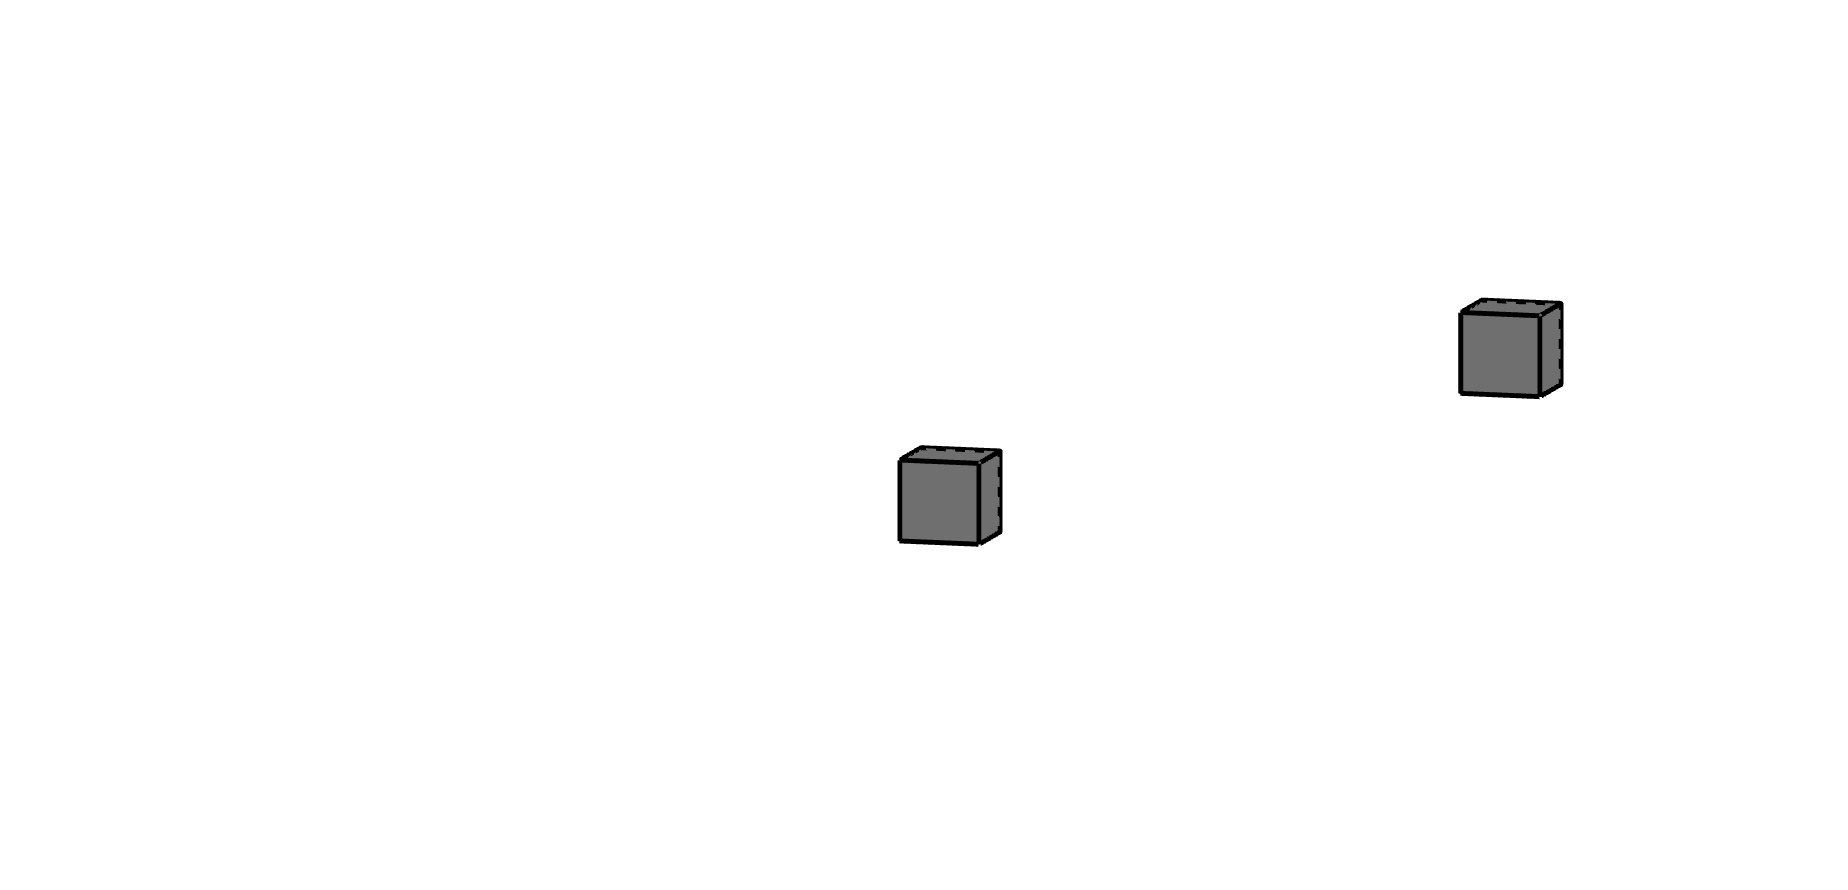
\includegraphics[width=1\textwidth,trim={10cm 0cm 3cm 0cm},clip]{slike/36_OrtogonalnaProjekcijaKuba.png}
	\captionsetup{justification=centering}
	\caption{Kocke dobivene korištenjem ortogonalne projekcije}
	\label{fig:OrtogonalnaProjekcijaKuba}
\end{figure}

Prikladnija projekcija bila bi perspektivna projekcija. Njenim korištenjem, objekti bliže kameri se povećavaju, a oni udaljeniji se smanjuju. Kao što je prije rečeno, frustum perspektivne projekcije izgleda kao frustum po definiciji. Ovakvim projiciranjem se sve 3D točke projiciraju na ravninu, no uzima se u obzir udaljenost točke od kamere. Slika \ref{fig:FrustumPerpspektivneProjekcije} daje bolji uvid u komponente tog frustuma. Za izradu matrice perspektivne projekcije potrebni su vidno polje (\textit{field of view} ili FoV), format prikaza (\textit{aspect ratio}), udaljenost od bliske odrezajuće ravnine \textit{zBlizu} (\textit{zNear}) i udaljenost od daleke odrezajuće ravnine \textit{zDaleko} (\textit{zFar}). FoV definira koliki dio "svijeta" je vidljiv, a izražen je kao kut. Na slici je prikazan narančastom bojom. Što je FoV veći to se više vidi prostora, no dolazi do lošije kvalitete prikaza objekata. Format prikaza je omjer širine i visine ekrana na kojemu se slika prikazuje. Loš omjer može dovesti do "spljoštene" ili rastegnute slike jer se njime pokušava prevesti "kvadratasta" slika u pravokutni ekran. Varijabla \textit{zBlizu} predstavlja udaljenost kamere od bliske odrezajuće ravnine na koju se projicira cijela slika. Ona je na slici predstavljena zelenom bojom. Sve točke koje se nalaze ispred te ravnine neće biti vidljive. Daleka odrezajuća ravnina \textit{zDaleko} je ljubičasta ravnina sa slike koja definira udaljenost od najudaljenije točke koja se može prikazati. Sve točke van frustuma se ne prikazuju, a one koje su unutar frustuma možemo zamisliti kao da se prikazuju na \textit{zBlizu} ravnini. Ovo je prikazano i na slici gdje se na zelenoj ravnini nalazi linija koja se stanjuje prema desno. Ta linija predstavlja pravac koji prolazi kroz frustum, ali samo jednim dijelom. Rozi dio tog pravca sa slike se neće vidjeti, a iscrtani dio se prikazuje \parencite{Perspective3DBezDat}. 

Matrica perspektivne projekcije \parencite{WebGPUFundamentalsPerspective} se intuitivno teško tumači:

\[
\begin{bmatrix}
	\frac{f}{aspekt} & 0 & 0 & 0 \\
	0 & f & 0 & 0 \\
	0 & 0 & zDaleko \cdot rangeInv & -1 \\
	0 & 0 & zBlizu \cdot zDaleko \cdot rangeInv & 0 \\
\end{bmatrix}
\]
\\Varijable koje prije spomenute su $f$ i $rangeInv$. Varijabla $f$ definira koliko će se cijela "scena", tj. sve prikazane točke, skalirati na osnovu FoV-a. Varijabla $f$ se tako temelji na FoV-u:

\begin{align*}
	f = \tan(\pi\cdot0.5 - 0.5\cdot FoV).
\end{align*}

Tangens funkcija se koristi jer FoV čini trokut između točke kamere, daleke odrezajuće ravnine \textit{zDaleko} i rubova ekrana na kojima će se točke prikazivati. Dalje, množenjem $\pi$ s 0.5 i oduzimanje 0.5 pomnoženog s FoV će dati kut između središta "ekrana" i njegovog vrha. Računanjem tangensa tog kuta, dobiti će se omjer baze i visine ranije spomenutog trokuta. Dalje, dijeljenjem varijable $f$ s aspektom prilagođava se faktor skaliranja na temelju formata prikaza ekrana. Ova vrijednost se koristi samo nad $x$ komponentom točke kako bi se objekti na ne-kvadratnim površinama svejedno normalno prikazivali. Na kraju, posljednja "nepoznata" varijable je \textit{rangeInv}. Ona služi kako bi se $z$ koordinata prevela iz globalnog u normalizirani prostor, odnosno prostor koji se kreće od -1 do 1. Važnost ovoga će se kasnije objasniti. Prva dva reda matrice se koriste kako bi se $x$ i $y$ koordinate pravilno skalirale na temelju udaljenosti točke od kamere i FoV-a. Ovako se $x$ i $y$ koordinate pravilno skaliraju kako bi bile manje što su dalje od kamere čime se stvara efekt perspektive. Treći red matrice se koristi za transformaciju $z$ koordinate i postavljanje $w$ komponente. Komponenta $zDaleko \cdot rangeInv$ skalira $z$ komponentu točke čime ju pretvara iz dubine definirane u globalnom prostoru u dubinu definiranu u NDC-u. Recimo, da je $z$ komponenta neke točke jednaka udaljenosti \textit{zBlizu} ili \textit{zDaleko}, djelovanjem ove vrijednosti dobila bi se vrijednost -1 ili 1. Tako su se zapravo $z$ komponente točaka skalirale u NDC prostor. Vrijednost -1 u tom redu matrice, u posljednjem stupcu, postavlja varijablu $w$ za "perspektivno dijeljenje". Kao što je ranije rečeno, $w$ komponenta se koristi kako bi se sve vrijednosti točke podijelile s njom čime se dobiva efekt percepcije. Vrijednost -1 osigurava da će $w$ poprimiti vrijednost $-z$ što je i potrebno za perspektivno dijeljenje. Posljednji red skalira $z$ komponentu i dalje, no ovaj put u odnosu na \textit{zBlizu} i \textit{zDaleko} vrijednosti. Ove kompleksne operacije se temelje na trigonometriji unutar frustuma i mogu biti relativno komplicirane za objasniti, no krajnji rezultat će svakako biti vjernija 3D vizualizacija nego korištenjem ortogonalne projekcije. Slika \ref{fig:PerspektivnaProjekcijaKuba} prikazuje kocke (koje su bile prikazane na slici \ref{fig:OrtogonalnaProjekcijaKuba}) čije su vizualizacije dobivene korištenjem perspektivne projekcije. Naravno, ovdje je očito da se jedna kocka nalazi dublje u sceni od druge zbog skaliranja njihovih veličina ovisno o $z$ komponentama.

\begin{figure}[H]
	\centering
	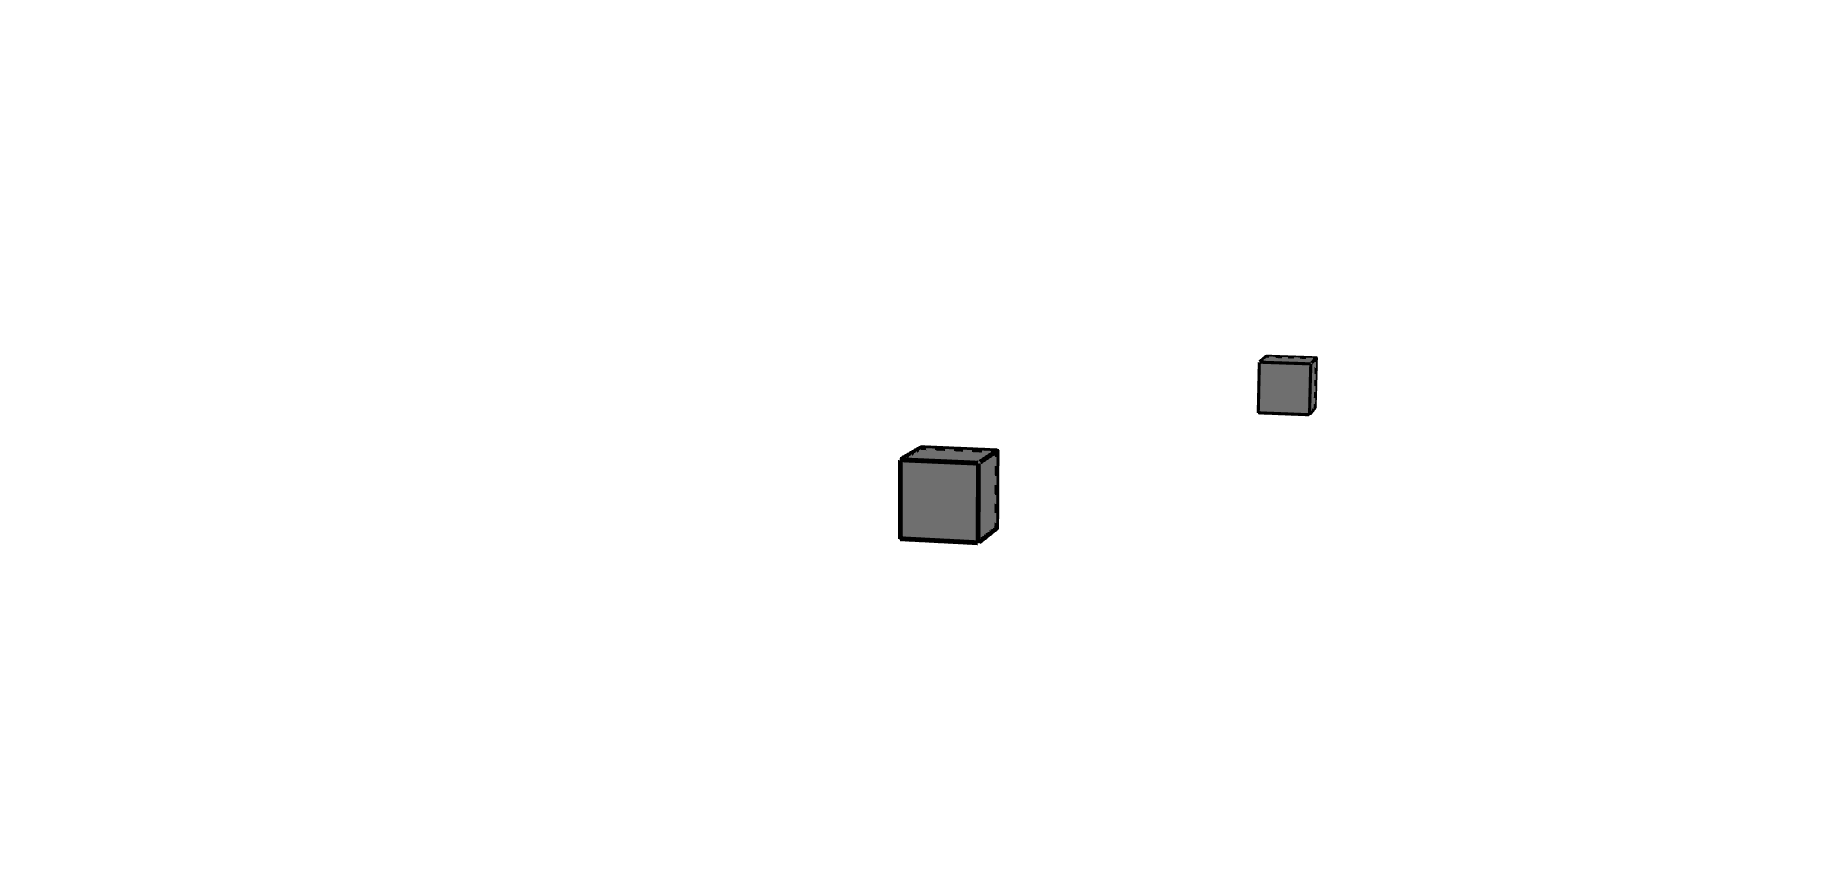
\includegraphics[width=0.95\textwidth]{slike/37_PerspektivnaProjekcijaKuba.png}
	\captionsetup{justification=centering}
	\caption{Kocke dobivene korištenjem perspektivne projekcije}
	\label{fig:PerspektivnaProjekcijaKuba}
\end{figure}

\subsection{Kamera}
Osim projiciranja svih objekata, potrebno je definirati kameru kojom će se moći kretati u prostoru i vidjeti eksplozija iz različitih kuteva. Matrica pogleda transformira koordinate iz globalnog prostora u prostor pogleda. Osim toga, ova matrica definira "pogled" na scenu. Ova transformacija je zaslužna za postavljanje kamere na određenu poziciju u prostoru i njeno usmjeravanje prema željenom objektu. U prostoru pogleda, kamera se nalazi u ishodištu. Kamera se definira pomoću pozicije kamere, pozicije objekta i pozicije vektora koji definira smjer "gore". Za početak, potrebno je dobiti $z$ os ovog koordinatnog sustava kamere. Ona se dobiva normalizacijom vektora koji nastaje oduzimanjem točke objekta od točke kamere. Zatim se provodi normalizacija. Time je definiran smjer u kojemu gleda kamera. Dalje, potrebno je definirati $x$ os koordinatnog sustava kamere. Ovaj vektor definira desnu orijentaciju kamere, odnosno osigurava da je kamera dobro pozicionirana u tri dimenzije. Ovaj vektor se dobiva računanjem vektorskog produkta vektora "gore" i dobivene $z$ osi koordinatnog sustava kamere. Na kraju, potrebno je dobiti $y$ os. On definira gornji smjer u koordinatnom sustavu kamere i osigurava da je smjer "gore" točno orijentiran i ortogonalan u odnosu na $x$ i $z$ osi. Definiranjem ovih vektora dobiven je novi koordinatni sustav. Dobivena matrica izgleda ovako:

\[
\begin{bmatrix}
	xOs_x & xOs_x & xOs_x & 0 \\
	yOs_x & yOs_x & yOs_x & 0 \\
	zOs_x & zOs_x & zOs_x & 0 \\
	kamera_x & kamera_y & kamera_z & 1 \\
\end{bmatrix}
\]

Prva tri reda predstavljaju vektore koji definiraju prostor pogleda. Ovom matricom je moguće dani vektor prevesti iz njegovog ortonormiranog sustava u prostor pogleda. Na taj način, svi objekti su definirani u odnosu na kameru. Posljednji red translatira kameru u središte koordinatnog sustava. No, zbog lakšeg baratanja svim koordinatama, moguće je napraviti inverz ove matrice. Umjesto da se kamera pomiče oko objekata, mogu se micati svi objekti oko kamere. Na taj način, lakše je raditi ostale transformacije nad tim objektima jer nisu definirani na osnovu svoje pozicije unutar sustava kamere, već je kamera definirana u odnosu na sustav u kojemu se koristi \parencite{KameraBezDat}.

Matrice pogleda i perspektive su osnova za rad u tri dimenzije. Sustav kamere će omogućiti kretanje kroz scenu eksplozije čestica, a perspektivno projiciranje će dovesti do realističnijih prikaza pojedinih čestica koje se kreću od ili prema kameri. Sljedeće, potrebno je pojasniti tehnologiju u kojoj se ove matrice planiraju koristiti.

\section{WebGPU}
3D transformacije su ekstremno zahtjevne za izvođenje, a pogotovo unutar programskih jezika kao što je JavaScript. Korištenjem raznih metoda optimizacije, moguće je pokrenuti neke vizualizacije koje prate stanje velikog broja pojedinih objekata, no u slučaju ove vizualizacije čestica, željeni broj vizualiziranih čestica je barem milijun. Iako se ovo čini kao previsok cilj za dostići, pogotovo u tri dimenzije, postoji računalna komponenta koja može uvelike pomoći u ovom pothvatu. Grafički procesor ili GPU je poseban procesor dizajniran za izvođenje ogromnog broja paralelnih operacija. Dok je glavni procesor efikasan u izvršavanju pojedinačnih zadataka, grafički procesor može izvoditi veliki broj jednostavnijih ponavljajućih zadataka. On je savršen za vizualizaciju velikog broja čestica koje prate iste zakonitosti i uz to su istog izgleda. No, programiranje procedura za izvođenje na grafičkom procesoru zahtjeva bolje razumijevanje paralelizma i upravljanja memorijom. JavaScript ima definirano nekoliko API-ja za rad s grafičkim procesorom unutar preglednika. Za ovaj projekt, odabran je WebGPU.  WebGPU je API koji omogućava korištenje grafičkog procesora za izvođenje kompleksnijih operacija i lakše crtanje velikog broja objekata. Sve što je potrebno za korištenje ovog API-ja je dohvaćanje priključka za GPU uređaj i dohvaćanje podataka o tom uređaju. Poznatiji API za rad s grafičkim procesorom je WebGL. WebGL je već ustaljen API koji koriste mnogi sustavi. Jednostavniji je za korištenje od WebGPU-a, ima veću zajednicu ljudi koja ga koristi i postoji duže. Unatoč tim prednostima, odabran je WebGPU. Njegova prednost nad WebGL-om je mogućnost pisanja \textit{compute shadera}. WebGPU je nastao 2011. godine i od onda ga podupire sve veći broj preglednika. Od nastanka, ima bolje performanse od WebGL-a, a i uvodi neka poboljšanja naspram WebGL-a kao što je bolje upravljanje stanjem \parencite{DocWebGPU}. 

Grafički procesori izvršavaju \textit{shadere}. Programi za sjenčanje, sjenčari ili \textit{shaderi} su programi koji se izvode unutar grafičkog procesora. Postoji nekoliko vrsta, a WebGPU podupire programe za sjenčanje vrhova (\textit{vertex shader}), programe za sjenčanje fragmenata (\textit{fragment shader}) i programe za računalne operacije (\textit{compute shader}). \textit{Vertex shader} je program koji se izvodi za svaki proslijeđeni vrh. Vrhovi su samo točke u prostoru koje izlaze kao rezultat izvođenja ovog \textit{shadera}. Njegovo izvođenje se događa prije izvođenja \textit{fragment shadera}. \textit{Fragment shader} je program koji se izvodi za svaki fragment ili piksel između vrhova. Svrha njegovog korištenja je da vraća boju svakog piksela koji se prikazuje. Ova dva \textit{shadera} se koriste za prikaz podataka, a \textit{compute shader} se najčešće koristi za izvođenja operacija koje nisu direktno vezane uz prikaz. U slučaju vizualizacije eksplozija čestica, oni će se koristiti za generiranje čestica i djelovanje silom na čestice. Ove operacije se mogu odvijati paralelno za svaku česticu i zato su savršene za izvođenje na \textit{compute shaderu}. Iako postoji još nekoliko vrsta \textit{shadera}, WebGPU podupire samo ove tri. Dodatno, potrebno je napomenuti kako se ove tri vrste ne mogu izvoditi proizvoljnim redom. \textit{Vertex} i \textit{fragment shaderi} se moraju izvoditi uzastopno, prvo \textit{vertex shader} obrađuje podatke vrhova, a zatim ih \textit{fragment shader} "crta", odnosno definira kako će biti nacrtani. \textit{Compute shaderi} se mogu izvoditi bilo kada, osim između izvođenja \textit{vertex} i \textit{fragment shadera} \parencite{WebGPUFundamentalsFundamentals}.

  
Svi \textit{shaderi} se pišu u posebnom jeziku za WebGPU. WGSL (\textit{WebGPU Shading Language}) je jezik za pisanje \textit{shadera} za WebGPU API u kojemu se mogu definirati dvije vrste naredbi za izvršavanje procedura na GPU. Jedna vrsta su naredbe za crtanje u kojima se definiraju \textit{vertex} i \textit{fragment shaderi}. Druga vrsta naredbe je \textit{dispatch} naredba kojom se definiraju \textit{compute shaderi}. Točnije bi bilo reći da ove dvije vrste naredbi omogućavaju izvršavanje dviju vrsti protočnih sustava (\textit{pipeline}), naredbe za iscrtavanje izvršavaju protočni sustavi za iscrtavanje (\textit{render pipeline})i \textit{dispatch} naredbe izvršavaju protočni sustav za računanje (\textit{compute pipeline}). Svaki protočni sustav definira koji \textit{shaderi} se trebaju izvesti, definira otkuda dolaze njihovi podaci, gdje se spremaju ili prosljeđuju rezultati i omogućava konfiguriranje dodatnih opcija. Slika \ref{fig:Pipelines} prikazuje pojednostavljeni prikaz jednostavnog WebGPU procesa. Cilj ovog malog programa je prikazati sinusoidu na ekranu. \textit{Compute shader} se izvodi prvi i vrši računanje pozicije točke u danom trenutku. On će nacrtati veliki broj čestica kako bi se nacrtala cijela sinusoida. Nakon toga, \textit{vertex shader} uzima poziciju dane točke i dodaje joj sve potrebne atribute, kao što je boja kojom će ona biti predstavljena na temelju pozicije. Na kraju, cijela točka se šalje u \textit{fragment shader} koji dalje prosljeđuje točku na crtanje. Slika \ref{fig:Pipelines} prikazuje ovaj jednostavan program \parencite{TourOfWGSL}. 

\begin{figure}[H]
	\centering
	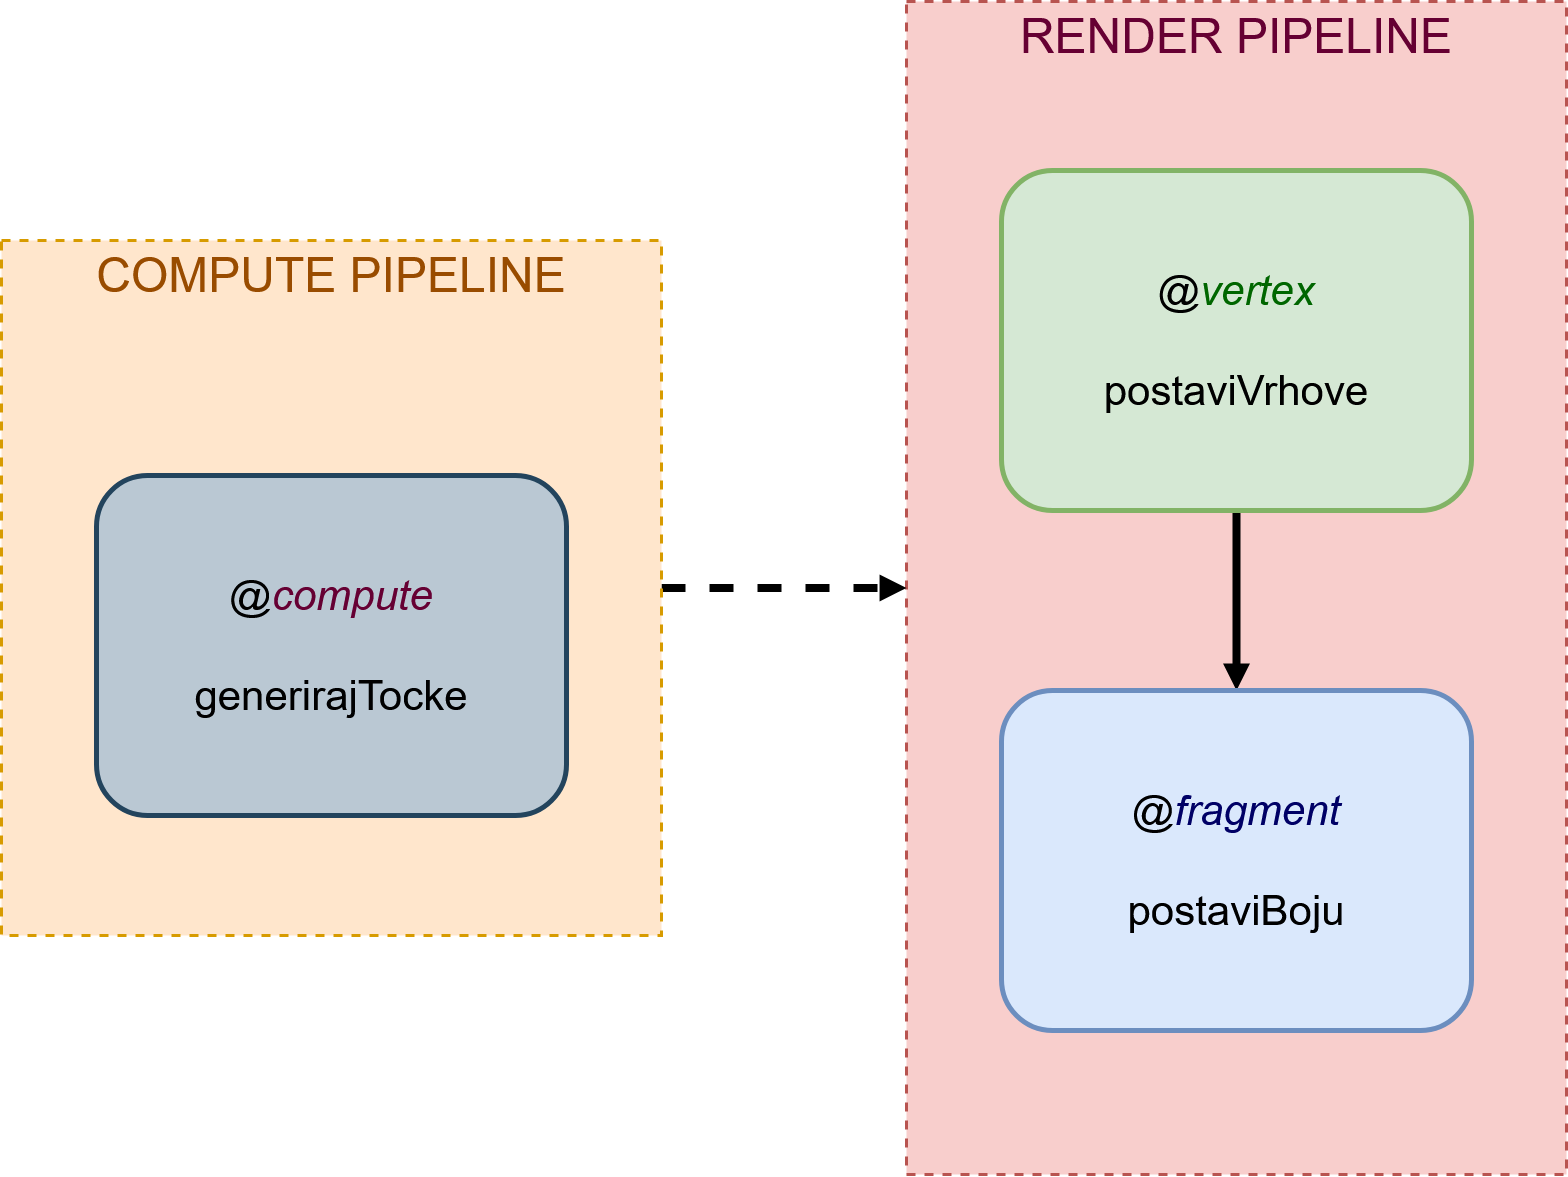
\includegraphics[width=0.95\textwidth]{slike/38_Pipelines.png}
	\captionsetup{justification=centering}
	\caption{Prikaz \textit{shadera} unutar protočnih sustava}
	\label{fig:Pipelines}
\end{figure}

 
Svi podaci koji se koriste u \textit{shaderima} pohranjuju se u spremnike (\textit{buffere}). U suprotnom nisu dostupni grafičkom procesoru. Tako \textit{shader} vidi samo podatke koji su mu eksplicitno proslijeđeni kroz spremnik. Postoji nekoliko različitih vrsta spremnika: spremnik vrhova (\textit{vertex buffer}), uniformni spremnik (\textit{uniform buffer}) i \textit{storage} spremnik. Spremnik vrhova je spremnik koji se može koristiti samo za pohranu podataka koje će čitati \textit{vertex shader}. Za razliku od drugih spremnika, ovom spremniku se direktno pristupa iz \textit{shadera}. Dovoljno je u definiciji funkcije specificirati da će neki parametar biti čitan iz spremnika vrhova. Podaci iz tog spremnika se tako mogu koristiti kao da su proslijeđeni parametri u \textit{vertex shader}. Ova vrsta spremnika se može koristiti kao ulaz u proces crtanja. Ako je potrebno dijeliti podatke kroz više različitih \textit{shadera} (koji mogu biti različite vrste), moguće je koristiti uniformni spremnik. Ovaj spremnik se može koristiti samo za čitanje podataka iz njega, a postavlja se prije izvođenja \textit{shadera}. Ovakvi spremnici su korisni za pohranu podataka koji se neće mijenjati kao što su razne konstante i matrice transformacija. No, nekada je potrebno pisati i čitati iz spremnika. Za to je potrebno koristiti \textit{storage} spremnik. Osim čitanja i pisanja, oni omogućavaju još neke opcije kao što je prosljeđivanje podataka van \textit{shadera}.  Osim ove tri vrste spremnika, postoje i posebne varijable koje se prosljeđuju između \textit{vertex} i \textit{fragment shadera}. Te vrijednosti su najčešće vrhovi koji se prosljeđuju u \textit{fragment shader} kako bi se mogli nacrtati. Kako bi \textit{shaderi} pristupili spremnicima, potrebno je eksplicitno proslijediti reference na te spremnike u protočne sustave u kojima su pozvani \textit{shaderi}. Reference se pohranjuju u vezne grupe resursa (\textit{bind groups}). Vezne grupe resursa predstavljaju način za prosljeđivanje referenci na resurse iz JavaScripta u WebGPU \textit{shadere} kao što su reference na spremnike \parencite{BufferTypes}. 

Kroz spremnike je moguće proslijediti različite tipove podataka. Za početak, osnovna 4 tipa su:

\begin{itemize}
	\item $f32$ - 32-bitni broj s pomičnim zarezom,
	\item $i32$ - 32-bitni cijeli broj,
	\item $u32$ - 32-bitni cijeli broj bez predznaka,
	\item $f16$ - 16-bitni broj s pomičnim zarezom.

\end{itemize}

Veličine ovih tipova podataka su vrlo bitne jer se na strani JavaScripta treba definirati točna veličina pojedinog spremnika. Ako je potrebno proslijediti četiri decimalna broja u sva tri \textit{shadera}, potrebno je definirati uniformni spremnik od 32 * 4 bita, odnosno spremnik od 16 bajtova. Vrijednosti se zatim pohranjuju u taj spremnik kao niz bitova koji se čitaju na strani \textit{shadera}. Ondje interpretacija tih bitova ovisi o tome kakve podatke očekuje \textit{shader}, a ako je s obje strane dobro definirano što se prosljeđuje, dobiti će se očekivani rezultat. Drugi tipovi podataka koji se mogu koristiti su \textit{vec2<T>}, \textit{vec3<T>}, \textit{mat2x2<T>}, \textit{mat2x3<T>} i tako dalje. Ovi tipovi su korisni za prosljeđivanje matrica i vektora u spremnike. Oni se sastoje od osnovnih tipova podataka. Naravno, osim ovih osnovnih tipova, mogu se definirati i strukture podataka s ključnom riječju "struct". Za postizanje ovoga, na JavaScript strani su definirani posebni objekti koji dobivene vrijednosti pretvaraju u nizove bitova. Osim toga, daju pristup pojedinim svojstvima tih nizova kao što je dobivanje veličine u bajtovima i slično. Ti tipovi podataka su \textit{ArrayBuffer}, \textit{Float32Array}, \textit{UInt8Array} i tako dalje. Svi ovi objekti se mogu inicijalizirati drugačijim konstruktorima, bilo to prosljeđivanjem broja koji predstavlja veličinu niza u bajtovima ili prosljeđivanjem konkretnih vrijednosti koje se tada pretvaraju u niz bitova. Jedan od problema koji otežava rad sa spremnicima je računanje veličine proslijeđenih podataka. Ako se radi samo o osnovnim tipovima podataka, vjerojatno neće biti problema, no kompleksnije strukture mogu dovesti do problema. Do toga najčešće dolazi zbog razmaka koji je potrebno uvesti u strukture kako bi se njihov sadržaj točno čitao. Svaka struktura u WebGPU-u ima svoja pravila za raspodjelu koja diktiraju gdje točno u memoriji neki podatak mora biti spremljen kako bi se pravilno čitao. Ovakvim strogim upravljanjem memorijom se može povećati efikasnost prilikom pristupanja memoriji. Ova pravila su različita za svaki tip podataka, no za dani tip podataka, poravnanje mora biti potencija broja 2. Na primjer, \textit{vec3<f32>}  može u sebi sadržavati maksimalno 12 bajtova podataka, no ovo krši pravilo poravnanja jer 12 nije potencija od 2. Iz tog razloga, potrebno je dodati 4 bajta razmaka prilikom pohrane podataka na strani JavaScripta. Ovakva pravila poravnanja je vrlo teško pratiti i dovodi do velikog broja grešaka ako ne postoji dobra metoda praćenja stanja. Iz tog razloga, za potrebe ovog rada korišten je alat za računanje razmaka: \url{https://webgpufundamentals.org/webgpu/lessons/resources/wgsl-offset-computer.html#}. Ovaj jednostavni program prima WGSL deklaraciju strukture podataka i za nju daje kod koji se može koristiti za popunjavanje te strukture na strani JavaScripta. Dodatni problem koji nije moguće riješiti je taj da ako se deklaracija strukture unutar WGSL koda promijeni, potrebno je tražiti deklaraciju vrijednosti koje će se spremiti u spremnik na strani JavaScripta i ažurirati ga. Ako se to ne napravi, vjerojatno se nigdje neće pojaviti greška već će se vrijednosti krivo čitati na strani \textit{shadera} \parencite{WebGPUFundamentalsMemoryLayout}.



Nakon što su definirani \textit{shaderi}, njihovi spremnici  i grupe kojima oni pripadaju, potrebno je definirati redoslijed i način izvršavanja \textit{shadera}. Ako se izvršavaju \textit{shaderi} za crtanje, potrebno je definirati fazu iscrtavanja (\textit{render pass}). U suprotnom, definira se faza računanja (\textit{compute pass}). Faza je skup naredbi koje se izvršavaju na GPU-u koristeći definirane \textit{shadere} i resurse koji su s njima povezani. Faza iscrtavanja predstavlja skup naredbi pomoću kojih se crta na platno (ili neku drugu teksturu), a faza računanja predstavlja skup naredbi za izvršavanje općenitih procesa definiranih \textit{compute shaderima}.  

U slučaju \textit{vertex} i \textit{fragment shadera}, broj dretvi koje se istovremeno izvode određuje GPU. Kako se \textit{compute shaderi} koriste za mnogo općenitije poslove, postoji mogućnost definiranja veličina radnih grupa (\textit{workgroups}). Radna grupa je skupina poziva dretvi koje se izvode istovremeno, a dijele pristup varijablama u adresnom prostoru tih radnih grupa. Unutar svakog poziva \textit{compute shadera}, može se pristupiti nekoliko ugrađenih varijabli kao što su:

\begin{itemize}
	\item \textit{local\_invocation\_id} - identificira dretvu unutar njene radne grupe,
	\item \textit{workgroup\_id} - predstavlja ID radne grupe povezan s trenutnom dretvom (odnosno ID je isti za sve dretve unutar jedne radne grupe),
	\item \textit{global\_invocation\_id} - jedinstveni ID za svaku dretvu kroz sve radne grupe \parencite{WebGPUFundamentalsMemoryLayout}.
\end{itemize}
Izvođenje \textit{compute shadera} kreće kada se naredbom definira i poziva radna skupina sastavljena od određenog broja dretvi. Dretve se tako mogu (ali ne moraju) izvoditi istovremeno, bez određenog redoslijeda i bez osiguranja da neka dretva neće spriječiti izvođenje ostalih. WebGPU garantira samo da će se proslijeđeni broj dretvi pokrenuti. Slika \ref{fig:Buffers} prikazuje kompletno izvođenje svih potrebnih \textit{shadera} i njihovo korištenje memorije iz primjera sa sinusoidom. Ponovo, prikazana su tri \textit{shadera}, no ovaj put su pokazani i tokovi podataka. Zelene strelice predstavljaju čitanje podataka, a crvene pisanje. \textit{Compute shader} prvo čita podatak \textit{vrijeme} iz uniformnog spremnika označenog plavom bojom. Nakon toga, računa \textit{poziciju te točke} koristeći sinus funkciju i pročitano vrijeme. Dobivenu točku pohranjuje u jednu od pozicija unutar polja \textit{tocke} koje je predstavljeno sivom bojom. Polje \textit{tocke} je \textit{storage} spremnik. Tri točkice označavaju da postoji još elemenata u nizu, no zbog veličine slike nisu prikazani. Svaka pozicija u polju \textit{tocke} predstavlja jednu varijablu koja je struktura tipa \textit{Tocka}. Svaka ta varijabla se sastoji od samo jednog atributa \textit{pozicija}, a svaki atribut \textit{pozicija} se sastoji od dvije varijable tipa \textit{f32}. Svaka varijabla zauzima 4 bajta, odnosno \textit{pozicija} zauzima 8 bajtova. \textit{pozicija} zapravo predstavlja 2D vektor, odnosno koordinate jedne točke. Brojevi iznad naziva spremnika \textit{vrijeme} i \textit{tocke} predstavljaju poziciju spremnika unutar grupe. Grupa je tako sačinjena od dva spremnika, a predstavljena je kvadratom obojenim plavom i sivom bojom. Sljedeći korak u izvođenju je prosljeđivanje vrijednosti u \textit{vertex shader}. Polje \textit{tocke} ima uključene tri zastavice, jednu koja označava spremnik kao \textit{storage} spremnik, jednu koja označava da se u njega može pisati i posljednju koja definira ovaj spremnik kao spremnik vrhova. Spremnik tako može imati više uloga unutar više protočnih sustava. \textit{Vertex shader} tako prima podatke iz spremnika vrhova \textit{tocke}, obrađuje ih, rezultat sprema u \textit{inter-stage} varijablu tipa \textit{VrhOutput} i prosljeđuje ga u \textit{fragment shader}. Daljnji tijek rada GPU-a nije prikazan, ali u njemu kreće crtanje po platnu.

\begin{figure}[H]
	\centering
	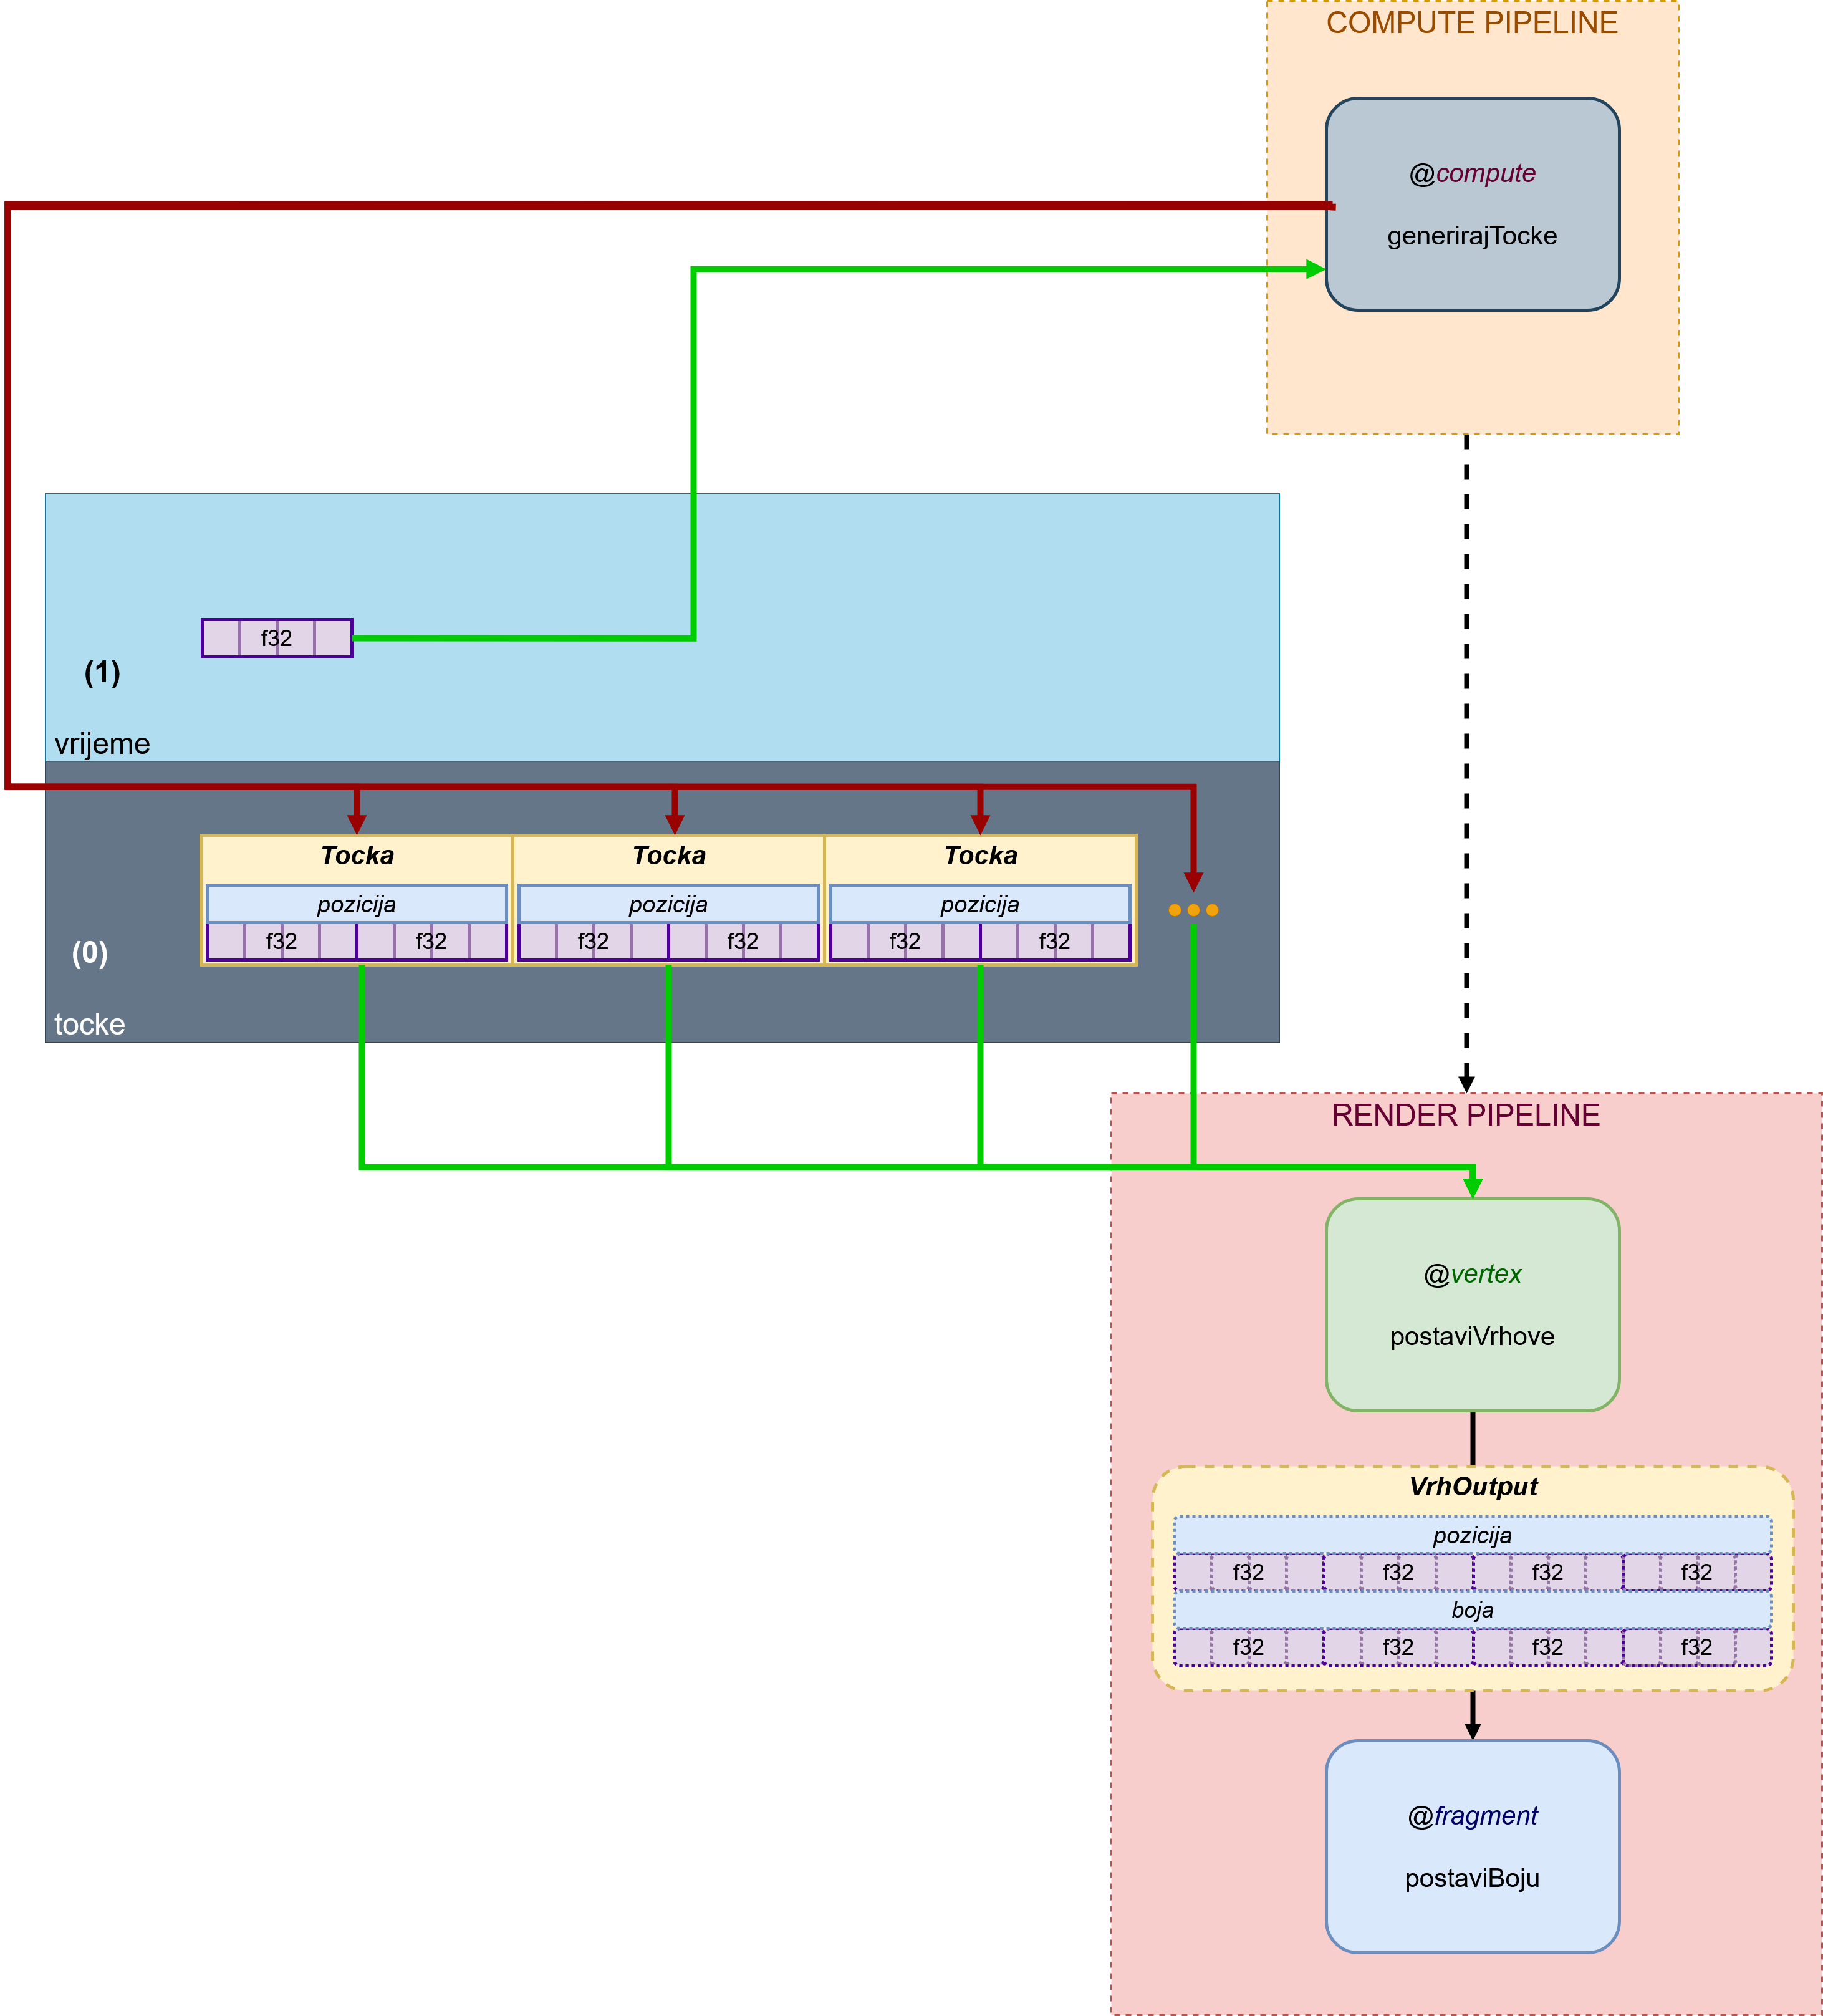
\includegraphics[width=0.95\textwidth]{slike/39_Buffers.png}
	\captionsetup{justification=centering}
	\caption{Prikaz procesa unutar GPU-a}
	\label{fig:Buffers}
\end{figure}


Na kraju, potrebno je spomenuti da grafički procesori imaju različite kapacitete, odnosno mogu imati manje ugrađene memorije, manje jezgri za izvođenje i slično. Iz tog razloga, WebGPU omogućava dohvaćanje adaptera za uređaj koji posjeduje željene karakteristike. WebGPU specificira "minimalni uređaj", odnosno specificira koje su karakteristike grafičkog procesora osigurane i na koje možemo uvijek računati. Na primjer, WebGPU osigurava da uređaj na kojemu se izvodi \textit{shader} može imati barem osam \textit{storage} spremnika po stadiju \textit{shadera}, odnosno toliko ih svaki \textit{shader} može koristiti. Kako bi vizualizacije bile dostupne na svim uređajima koji podržavaju WebGPU, koristit će se ova minimalna ograničenja. To znači da treba posebno obratiti pažnju na upravljanje memorijom kako bi se maksimizirao broj čestica koje će se prikazati \parencite{WebGPUFundamentalsOptionalLimits}.
 
Tijek rada WebGPU-a je tada dohvaćanje priključka (adaptera) za GPU, definiranje WGSL koda za \textit{shadere}, definiranje spremnika, definiranje protočnog sustava, postavljanje spremnika unutar protočnog sustava i postavljanje faze iscrtavanja ili računanja. Na kraju se definirani kod izvršava unutar GPU-a. Za lakše shvaćanje svih spomenutih koncepata, napravljen je primjer u kodu čiji rezultat je prikazan na slici \ref{fig:WebGPUSinusoida}

\begin{figure}[H]
	\centering
	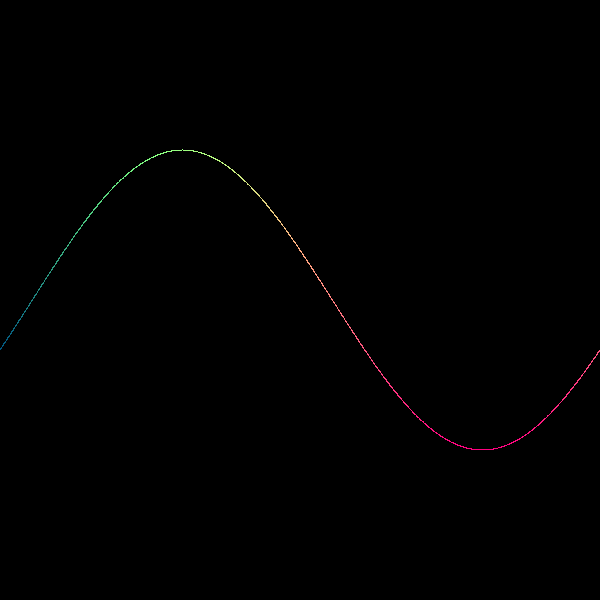
\includegraphics[width=0.95\textwidth]{slike/40_WebGPUSinusoida.png}
	\captionsetup{justification=centering}
	\caption{Animacija sinusoide napravljena koristeći WebGPU, JavaScript i WGSL}
	\label{fig:WebGPUSinusoida}
\end{figure}

WGSL kod za \textit{compute shader} (ali i ostale \textit{shadere}) napisan je kao teskt unutar JavaScripta. Kod glasi:

\begin{minted}{js}
const computeShaderWGSL = `
struct Tocka {
	pozicija: vec2<f32>,
}

@group(0) @binding(0) var<storage, read_write> tocke: array<Tocka>;
@group(0) @binding(1) var<uniform> vrijeme: f32;

@compute @workgroup_size(64)
fn generirajTocke(@builtin(global_invocation_id) global_id: vec3<u32>) {
	let index = global_id.x;
	if (index >= arrayLength(&tocke)) {
		return;
	}
	let x = f32(index) / f32(arrayLength(&tocke)) * 2.0 * 3.14159;
	let y = sin(x + vrijeme);
	tocke[index].pozicija = vec2<f32>(x / 3.14159 - 1.0, y * 0.5);
}
`;

const vertexShaderWGSL = `
struct VrhOutput {
	@builtin(position) pozicija: vec4<f32>,
	@location(0) boja: vec4<f32>,
}

@vertex
fn postaviVrhove(@location(0) pozicija: vec2<f32>) -> VrhOutput {
	var out: VrhOutput;
	out.pozicija = vec4<f32>(pozicija, 0.0, 1.0);
	out.boja = vec4<f32>(pozicija.x + 1.0, pozicija.y + 0.5, 0.5, 1.0);
	return out;
}
`;
const fragmentShaderWGSL = `
@fragment
fn postaviBoju(@location(0) boja: vec4<f32>) -> @location(0) vec4<f32> {
	return boja;
}
`;
\end{minted}

\textit{Compute shader} prvo definira strukturu \textit{Tocka} koja u sebi ima pohranjenu varijablu tipa \textit{vec2<f32>} nazvanu \textit{pozicija}. Dalje, anotacijama \textit{@group} i \textit{@binding} označeno je na koji način su podaci proslijeđeni u \textit{shader}. Anotacija \textit{@group} označava indeks vezne grupe resursa, a \textit{@binding} označava indeks na kojemu se spremnik nalazi unutar grupe. Kao što se vidi iz deklaracije, korišteni su \textit{storage} spremnik \textit{tocke} u kojemu će biti pohranjene sve točke koje će se crtati i uniformni spremnik \textit{vrijeme} u koji će se pohraniti dani trenutak za koji je potrebno nacrtati točke. Anotacija \textit{@compute}, kao i anotacije \textit{@vertex} i \textit{@fragment}, definira vrstu \textit{shadera} koji će implementira. Veličina radne grupe se definira anotacijom \textit{@workgroup\_size}. Posljednja anotacija korištena u \textit{compute shaderu} je \textit{@builtin} kojom se označava da je parametar \textit{global\_invocation\_id} jedinstveni indeks dretve. Ovoj vrijednosti se pristupa koristeći anotaciju, a služi kako bi se odredilo kojoj točki u polju će se pristupiti, točnije, gdje će se ona pohraniti. Ostatak koda je već objašnjen, računaju se koordinate točke koristeći dano vrijeme i sinus funkciju.

Dalje, definirani su \textit{vertex} i \textit{fragment shaderi} gdje \textit{vertex shader} za danu poziciju točke generira četverodimenzionalni vektor za poziciju i četverodimenzionalni vektor za boju koji se koriste za crtanje dane točke, a \textit{fragment shader} samo prosljeđuje dobivenu boju dalje u daljnje faze crtanja.  Prvo, definirana je struktura \textit{VrhOutput} koja se sastoji od varijabli \textit{pozicija} i \textit{boja}. Anotacija \textit{@builtin} ovdje definira da varijabla \textit{pozicija} predstavlja ugrađeni tip varijable koji služi za određivanje gdje će se točka crtati na ekranu. Anotacija \textit{@location} se može protumačiti kao definiranje indeksa na koji će se vrijednost spremiti u \textit{inter-stage} varijabli. Tako je označeno da će se ova vrijednost proslijediti dalje u \textit{fragment shader}. Ponovno, koristi se anotacija \textit{@location}, no ona se koristi ispred parametra što označava da se dani parametar čita iz spremnika vrhova s definirane pozicije. U \textit{fragment} \textit{shaderu}, ponovno se koristi ista anotacija i ponovno ima novo značenje. Ona ovdje označava da se dani parametar čita iz \textit{inter-stage} varijable s pozicije 0.

Osim definiranja WGSL koda, potrebno je postaviti okolinu za izvođenje \textit{shadera}. Na početku se dohvaćaju priključak i uređaj na kojemu će se izvoditi \textit{shaderi}. Potrebno je i konfigurirati kontekst tako da se specificira format teksture na kojoj će se izvoditi crtanje. Ovdje je definiran format u kojemu je svaka točka predstavljena crvenom, zelenom i plavom bojom te s prozirnosti. Svaka ta komponenta se sastoji od 8 bitova. Dodatno, definira se i \textit{alphaMode} koji definira uračunava li se "prozirnost" pri crtanju:


\begin{minted}{js}
const canvas = document.getElementById("container");
const context = canvas.getContext("webgpu");
const adapter = await navigator.gpu.requestAdapter();
const device = await adapter.requestDevice();

context.configure({
	device: device,
	format: "bgra8unorm",
	alphaMode: "premultiplied",
});
\end{minted}
  
Dalje, definiraju se spremnici i način njihovog korištenja te veličina u bajtovima:
\begin{minted}{js}
const brTocaka = 256 * 10;

const tockeVertexStorageBuff = device.createBuffer({
	size: brTocaka * 8,
	usage:
	GPUBufferUsage.STORAGE |
	GPUBufferUsage.VERTEX |
	GPUBufferUsage.COPY_DST,
});

const vrijemeUnifBuff = device.createBuffer({
	size: 4,
	usage: GPUBufferUsage.UNIFORM | GPUBufferUsage.COPY_DST,
});

\end{minted}

Idući korak je kompajliranje WGSL koda koji je ranije definiran. Za to se poziva funkcija \textit{createShaderModule} koja dani tekst pretvara u modul koji se može izvoditi unutar protočnog sustava:

\begin{minted}{js}
const computeShaderModule = device.createShaderModule({
	code: computeShaderWGSL,
});

const vertexShaderModule = device.createShaderModule({
	code: vertexShaderWGSL,
});

const fragmentShaderModule = device.createShaderModule({
	code: fragmentShaderWGSL,
});
\end{minted}

Dane spremnike je potrebno povezati s njihovim veznim grupama resursa tako da se definira shema koja sadrži opis spremnika na danom indeksu. Zatim se kreira vezna grupa resursa u kojoj se točno specificira koji spremnik će se povezati na koji indeks:

\begin{minted}{js}
const bindGroupLayout = device.createBindGroupLayout({
	entries: [
	{
		binding: 0,
		visibility: GPUShaderStage.COMPUTE,
		buffer: { type: "storage" },
	},
	{
		binding: 1,
		visibility: GPUShaderStage.COMPUTE,
		buffer: { type: "uniform" },
	},
	],
});

const bindGroup = device.createBindGroup({
	layout: bindGroupLayout,
	entries: [
	{ binding: 0, resource: { buffer: tockeVertexStorageBuff } },
	{ binding: 1, resource: { buffer: vrijemeUnifBuff } },
	],
});
\end{minted}


Napokon, definiraju se dva protočna sustava koji definiraju shemu izvođenja \textit{shadera}. Ovdje se specificira koje module je potrebno pozvati, koje vezne grupe resursa se vežu za koji \textit{shader} i još neke dodatne postavke. Jedna od njih je i \textit{primitives:\{topology:"point-list"\}}. Ona definira kako će se crtati dobivene točke. Dana postavka govori da će se svaka točka crtati kao jedan piksel na ekranu. Postoje i neke druge postavke koje definiraju da se svaka sljedeća točka treba povezati linijom (\textit{line-strip}) ili da svake tri točke čine trokut (\textit{triangle-list}):

\begin{minted}{js}
const computePipeline = device.createComputePipeline({
	layout: device.createPipelineLayout({
		bindGroupLayouts: [bindGroupLayout],
	}),
	compute: {
		module: computeShaderModule,
		entryPoint: "generirajTocke",
	},
});

const renderPipeline = device.createRenderPipeline({
	layout: "auto",
	vertex: {
		module: vertexShaderModule,
		entryPoint: "postaviVrhove",
		buffers: [
		{
			arrayStride: 8,
			attributes: [
			{ shaderLocation: 0, format: "float32x2", offset: 0 },
			],
		},
		],
	},
	fragment: {
		module: fragmentShaderModule,
		entryPoint: "postaviBoju",
		targets: [{ format: "bgra8unorm" }],
	},
	primitive: { topology: "point-list" },
});
\end{minted}

\textit{Shaderi} su sada spremni za izvođenje. Potrebno je još definirati fazu za iscrtavanje i računanje kako bi se pokrenuli definirani procesi. Prvo, poziva se \textit{commandEncoder} koji upravlja pozivanjem i postavljanjem svih resursa unutar GPU-a. Dvije bitne naredbe koje se prikazuju u kodu su \textit{draw} i \textit{dispatchWorkgroups}. Naredba \textit{draw} poziva \textit{vertex} i \textit{fragment shadere} da se izvedu $x$ puta. Naredba \textit{dispatchWorkgroups} poziva $x$ radnih skupina da se izvedu na grafičkom procesoru \parencite{W3CWebGPU2024}. Dodatno, prije definiranja faza, u spremnik za vrijeme je pohranjeno trenutno "vrijeme", odnosno vrijednost iteratora \textit{i} i pozvana je naredba \textit{requestAnimationFrame} kako bi se izvela animacija crtanja sinusoide:

\begin{minted}{js}
let i = 0;
function slicica() {
	const vrijeme = (i++) / 125;
	device.queue.writeBuffer(
	vrijemeUnifBuff,
	0,
	new Float32Array([vrijeme])
	);
	
	const commandEncoder = device.createCommandEncoder();
	
	const computePass = commandEncoder.beginComputePass();
	computePass.setPipeline(computePipeline);
	computePass.setBindGroup(0, bindGroup);
	computePass.dispatchWorkgroups(Math.ceil(brTocaka / 64));
	computePass.end();
	
	const renderPass = commandEncoder.beginRenderPass({
		colorAttachments: [
		{
			view: context.getCurrentTexture().createView(),
			loadOp: "clear",
			storeOp: "store",
			clearValue: { r: 0.0, g: 0.0, b: 0.0, a: 1.0 },
		},
		],
	});
	renderPass.setPipeline(renderPipeline);
	renderPass.setVertexBuffer(0, tockeVertexStorageBuff);
	renderPass.draw(brTocaka);
	renderPass.end();
	
	device.queue.submit([commandEncoder.finish()]);
	requestAnimationFrame(slicica);
}

requestAnimationFrame(slicica);
\end{minted}




\chapter{3D vizualizacija} 
Napokon, došlo je vrijeme za transformaciju 2D Coulombove eksplozije u 3D Coulombovu eksploziju. Prije upoznavanja sa \textit{shaderima}, potrebno je ponovno posjetiti model čestice. Očito, svaka čestica će ponovno biti predstavljena pozicijom, masom i brzinom. No čestice više neće biti pikseli jer pikseli nemaju 3 dimenzije. Ovdje je ponovno bilo moguće odabrati oblike kao što su možda kugle ili kocke. Problem s tim pristupom je način crtanja takvih objekata u tri dimenzije. U tri dimenzije, nije tako jednostavno za nacrtati složenije oblike od trokuta. Na primjer, umjesto crtanja kvadrata, potrebno je nacrtati dva trokuta koja će činiti kvadrat. Tako bi za crtanje jedne kocke bilo potrebno računati pozicije osam točaka koje čine šest strana točke. Svaka strana se mora sastojati od dva trokuta, stoga je u suštini potrebno nacrtati dvanaest trokuta da bi se nacrtala samo jedna čestica. Svaki trokut mora biti definiran s tri vrha što znači da se treba procesirati minimalno 36 vrhova. Kugle prividno nemaju nijednu stranicu, a i dovoljno je definirati samo promjer i središte kružnice da bi se ona mogla nacrtati. Ovo pretpostavka je kriva jer se kugla mora sastojati od trokuta kako bi se mogla nacrtati koristeći WebGPU. To znači da se crtanjem velikog broja trokuta koji prate oblik kugle može nacrtati jedna kugla. Što je broj trokuta veći, to oblik više naliči na kuglu. Ovdje je broj trokuta mnogo veći, ovisno o tome koliko "glatka" kugla se pokušava nacrtati. Ipak, odabran je najjednostavniji 3D oblik koji se može nacrtati. To je pravilna četverostrana piramida. Za njeno crtanje potrebno je definirati samo 4 točke koje se povezuju kako bi činile četiri trokuta. Sada je potrebno samo nacrtati četiri povezana trokuta i čestica je prikazana na ekranu. Ovakva čestica se prvo definira u JavaScriptu, prosljeđuje se u WebGPU spremnik i unutar \textit{shadera} se kopira koliko puta je potrebno. Dalje, središte ove piramide je u ishodištu koordinatnog sustava, a sve ostale piramide su samo kopije te piramide čiji vrhovi su translatirani za neku točku. Na ovaj način, nije potrebno generirati čestice unutar JavaScripta i sve ih proslijediti u WebGPU \textit{shadere}. Taj proces bi predstavljao ogroman korak unazad što se tiče performansi. Kod koji predstavlja piramidu (odnosno česticu) definiran je kao funkcija koja generira tri podatka: listu koordinata točaka, listu boja i broj vrhova piramide. Sama funkcija u sebi sadrži početne koordinate četiriju točaka, indekse koji tumače kojim redoslijedom je potrebno povezati dane vrhove kako bi se nacrtala piramida i vrijednosti boja za svaki vrh. Zatim, petljom se točke zapisuju u novu listu, ovaj put redoslijedom kojim je potrebno povezivati točke da se dobiju četiri stranice piramide. Osim toga, za svaku točku se definira njena boja. Dobivena lista koordinata će se sastojati od 48 brojeva gdje svaka četiri broja predstavljaju jednu točku. Isto tako, vrijednost boje svake točke je zapisana u drugu listu gdje se ponovo nalazi 48 vrijednosti, a svake četiri vrijednosti predstavljaju boju jedne čestice \parencite{WebGPUFundamentalsCameras}:

\begin{minted}{js}
function definirajCesticu() {
	let osnovnaKoordinata = 7;
	const koordinate = [
	//A
	osnovnaKoordinata,
	osnovnaKoordinata,
	osnovnaKoordinata,
	
	//B
	osnovnaKoordinata,
	-osnovnaKoordinata,
	-osnovnaKoordinata,
	//C
	-osnovnaKoordinata,
	osnovnaKoordinata,
	-osnovnaKoordinata,
	//D
	-osnovnaKoordinata,
	-osnovnaKoordinata,
	osnovnaKoordinata,
	];
	
	const indeksi = [
	//ABC
	0, 1, 2,
	//ADB
	0, 3, 1,
	//ACD
	0, 2, 3,
	//BDC
	1, 3, 2,
	//4
	];
	
	const boje = [
	/*
	//rozna
	200, 70, 120,
	//zuta
	200, 200, 0,
	//plava
	70, 120, 200,
	//zelena
	120, 200, 70,
	*/
	//orange1
	255, 135, 60,
	//orange1
	255, 115, 0,
	//orange1
	255, 105, 20,
	//orange1
	255, 145, 60,
	];
	
	const brojVrhova = indeksi.length;
	const podaciKoordinata = new Float32Array(brojVrhova * 4);
	const podaciBoja = new Float32Array(brojVrhova * 4);
	
	for (let i = 0; i < indeksi.length; ++i) {
		let skaliraniIndexPozicije = indeksi[i] * 3;
		const pozicija = koordinate.slice(
		skaliraniIndexPozicije,
		skaliraniIndexPozicije + 3
		);
		pozicija.push(1);
		podaciKoordinata.set(pozicija, i * 4);
		
		let skaliraniIndexBoje = Math.floor((i * 3) / 9) * 3;
		const boja = [
		boje[skaliraniIndexBoje] / 255,
		boje[skaliraniIndexBoje + 1] / 255,
		boje[skaliraniIndexBoje + 2] / 255,
		255 / 255,
		];
		podaciBoja.set(boja, i * 4);
	}
	console.log(podaciBoja);
	return {
		podaciKoordinata: podaciKoordinata,
		podaciBoja: podaciBoja,
		brojVrhova: brojVrhova,
	};
}
\end{minted}


\begin{figure}[H]
	\centering
	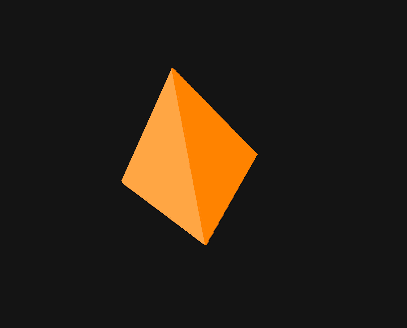
\includegraphics[width=0.95\textwidth]{slike/41_Cestica.png}
	\captionsetup{justification=centering}
	\caption{Prikaz 3D čestice (piramide)}
	\label{fig:Cestica}
\end{figure}

Nacrtana čestica sa slike \ref{fig:Cestica} je cijela narančasta, no svaka strana je druge nijanse narančaste kako bi se lakše vidjele različite strane piramide. Nakon kratkog prikaza čestice i opisa rada s njom, lakše će biti shvatiti kako rade \textit{shaderi} za vizualizaciju eksplozije.

\section{Shaderi}
Za razumijevanje vizualizacija, potrebno je objasniti svaki \textit{shader} pojedinačno, zašto su potrebni i zašto su implementirani kako su implementirani. \textit{Shaderi} implementiraju iste koncepte kao i 2D vizualizacije. Ponovno, potrebno je prvo generirati skup čestica koje prate Gaussovu razdiobu i na njih djelovati potencijalom koji će im postaviti početne brzine. Ovaj početni korak se izvodi samo jednom, a svi ostali koraci se ponavljaju "u nedogled". Prvo, računaju se pozicije čestica, nakon čega se one crtaju. Zato je potrebno napraviti nekoliko \textit{compute shadera} i samo jedan \textit{vertex} i \textit{fragment shader}.

\subsection{Compute shaderi}
Za vizualizaciju eksplozija potrebno je definirati dva odvojena \textit{compute shadera}, jedan za generiranje i početno djelovanje potencijalom na čestice i drugi za računanje iduće pozicije i utjecaja gravitacije i otpora na česticu. 

Za generiranje čestica i dobivanje Gaussove distribucije bilo je dovoljno koristiti ugrađenu \textit{Math.random()} metodu s primjenom Box-Mullerove transformacije nad njenim rezultatima. U slučaju WebGPU-a, ne postoji ugrađena metoda za generiranje nasumičnih brojeva. WebGPU je više fokusiran na provođenje paralelizma i crtanje pomoću danih podataka, a ne toliko na pružanje pomoćnih funkcija za programiranje. Iz tog razloga, potrebno je napraviti vlastitu implementaciju pseudonasumičnog generatora brojeva. Takvi generatori stvaraju nizove brojeva koji izgledaju kao da su nasumični, ali teoretski bi se cijeli niz mogao predvidjeti uz dovoljan broj informacija o metodi generiranja brojeva. Odabrana je implementacija hibridnog Tausworthe generatora. Tausworthe generator spaja više nasumičnih nizova brojeva kako bi dobio jedan veći niz. Temelji se na bitovnim operacijama kao što su pomak i XOR. Ta metoda je dovoljno dobra za generiranje nasumičnih brojeva, no moguće je da se tijekom generacije brojeva krenu prikazivati određeni uzorci u generiranju. Da bi se ovakvi neželjeni rezultati uklonili, Tausworthe generator se kombinira s još jednim generatorom. Drugi generator se naziva linearno kongruentni generator (LCG). Oba generatora su prigodna za paralelno izvođenje jer ne zahtijevaju poznavanje prijašnjih generiranih vrijednosti, odnosno to su generatori bez stanja. U implementaciji, prvo je potrebno definirati spremnike iz kojih će se čitati potrebni podaci i u koje će se spremati rezultati generiranja:

\begin{minted}{wgsl}
struct Parametri{
	dt:f32,
	otpor:f32,
	gravitacija:f32,
	pozicija_eksplozije:vec3f,
	snaga_potencijala:f32,
	radijus_cestica:f32,
}

const pi: f32 = 3.1415926535897932384626433832795;
@group(0) @binding(0) var<uniform> seeds: vec4<u32>;
@group(0) @binding(1) var<uniform> parametri: Parametri;
@group(0) @binding(2) var<storage, read_write> x_koordinate: array<f32>;
@group(0) @binding(3) var<storage, read_write> y_koordinate: array<f32>;
@group(0) @binding(4) var<storage, read_write> z_koordinate: array<f32>;
@group(0) @binding(5) var<storage, read_write> x_brzina: array<f32>;
@group(0) @binding(6) var<storage, read_write> y_brzina: array<f32>;
@group(0) @binding(7) var<storage, read_write> z_brzina: array<f32>;
\end{minted}

Struktura \textit{Parametri} pohranjuje osnovne postavke vizualizacije kao što su vremenski korak $dt$, koeficijent otpora, sile teže i potencijala, točku iz koje eksplozija kreće i polumjer generiranja čestica. Ove varijable su postavljene kao parametri kako bi se mogle definirati unutar preglednika i proslijediti u vizualizaciju. Dalje, definirana je konstanta $pi$. Za svaki slučaj, stavljeno je i više nego dovoljno decimala kako se ne bi izgubilo previše na preciznosti pri računanju. Prva dva spremnika su uniformni spremnici koji služe samo za čitanje dobivenih podataka iz JavaScripta. Svi spremnici se nalaze u istoj grupi na različitim indeksima. Prvo, definiran je vektor \textit{seeds}. On predstavlja četiri ključa ili sjemena na kojima se temelji pseudonasumična generacija brojeva. Kako bi se svakim novim izvođenjem vizualizacije kreirale čestice s drugačijim koordinatama, na strani JavaScripta se generiraju četiri velika nasumična broja koji će postati ključevi za hibridni generator brojeva. Dalje, u varijablu \textit{parametri} pohranjuju se ranije spomenuti parametri za izvođenje vizualizacije. Sljedećih šest spremnika predstavlja poziciju i brzinu čestice u danom trenutku. Pojedine vrijednosti iz polja \textit{x\_koordinate}, \textit{y\_koordinate}, \textit{z\_koordinate} predstavljaju vektor pozicije čestice. Točnije, predstavljaju točku za koju će se pomaknuti osnovna piramida definirana ranije na strani JavaScripta. Isto tako, pojedine vrijednosti iz polja \textit{x\_koordinate}, \textit{y\_koordinate}, \textit{z\_koordinate} predstavljaju vektor brzine čestice. Pristupanjem istom indeksu u svih šest polja dobiva se reprezentacija čestice. Očito, WebGPU podržava strukture podataka i semantički bi bilo smislenije napraviti posebnu strukturu koja će sadržavati sve potrebne informacije o čestici. Varijable predstavljene tom strukturom bi bile pohranjene u samo jedno polje. Glavna mana ovog pristupa je veliko zauzeće prostora u pojedinom spremniku. Maksimalna količina podataka koja se može pohraniti u \textit{storage} spremnik je 128 MB što je teoretski dovoljno za pohranu i više od milijun čestica predstavljenih strukturom od 24 bajta (4 bajta za svaku komponentu vektora brzine i pozicije). Točnije, može se pohraniti $\frac{128\cdot 1024^2}{24}$ čestica, odnosno preko pet milijuna čestica. Unatoč tome, jedan od ciljeva ove simulacije je odlična performansa zbog čega se želi maksimizirati količina čestica koje se mogu generirati. Razdvajanjem komponenti čestice na pojedine spremnike, moguće je pohraniti $\frac{128\cdot 1024^2}{4}$ čestica, što je preko trideset milijuna čestica. Očito, memorija neće biti problem za izvođenje željene vizualizacije.

Prve funkcije koje je potrebno implementirati su ranije spomenuti generatori. Njihova implementacija se temelji na statističkim zakonitostima. Ukratko, funkcija \textit{hybridTaus} spaja rezultat triju koraka Tausworthe generatora i rezultat LCG generatora. Tausworthe generator prima ključ, korake za pomak bitova ($S_1$, $S_2$, $S_3$) i bitovnu masku ($M$). LCG prima skalar množenja \textit{lcgStep} i konstantu za povećanje vrijednosti \textit{C} \parencite{NvidiaPRNG}:

\begin{minted}{wgsl}
fn tausStep(z: u32, S1: u32, S2: u32, S3: u32, M: u32) -> u32 {
	let b = (((z << S1) ^ z) >> S2);
	return (((z & M) << S3) ^ b);
}

fn lcgStep(z: u32, A: u32, C: u32) -> u32 {
	return A * z + C;
}

fn hybridTaus(z1: u32, z2: u32, z3: u32, z4: u32) -> f32 {
	let t1 = tausStep(z1, 13u, 19u, 12u, 4294967294u);
	let t2 = tausStep(z2, 2u, 25u, 4u, 4294967288u);
	let t3 = tausStep(z3, 3u, 11u, 17u, 4294967280u);
	let lcg = lcgStep(z4, 1664525u, 1013904223u);
	
	let combined = t1 ^ t2 ^ t3 ^ lcg;
	return f32(combined) * 2.3283064365387e-10;
}
\end{minted}

Dobivene vrijednosti je potrebno normalizirati na vrijednosti od -1 do 1. Ova normalizacija se provodi radi dobivanja podataka s kojima je lakše raditi\parencite{NormalizacijaPodataka}:
\begin{minted}{wgsl}
fn normaliziraj(vrijednost:f32)-> f32{
	var vrijednost_slozena:f32 = vrijednost;
	let rmin:f32 = -6;
	let rmax:f32 = 6;
	let tmin:f32 = -1;
	let tmax:f32 = 1;
	var norm:f32 = (((vrijednost_slozena-rmin)/(rmax-rmin))*(tmax-tmin))+tmin;
	if(norm>tmax){ return tmax;}
	else if(norm<tmin){ return tmin;}
	return norm;
}
\end{minted}

Ostale pomoćne funkcije su već definirane u dvije dimenzije. Funkcija \textit{djelujPotencijalom} računa rezultantnu silu kojom potencijal djeluje na generiranu česticu. Slično, funkcije \textit{djelujGravitacijom} i \textit{djelujOtporom} računaju rezultantne sile kojima sila teža i otpor sredstva djeluju na česticu. U implementacijama ovih funkcija se koristi parametar \textit{dretva\_id}. Koristeći taj parametar, pristupa se komponentama čestice. Ovaj parametar će biti jedinstven za svaku dretvu koja se izvodi, a kreće se od 0 do $x$ gdje $x$ predstavlja ukupan broj dretvi umanjen za jedan.  Funkcija \textit{pomakni\_cesticu} je slična funkciji  \textit{pomakni(dt, rezultantnaSila)} koja je implementirana ranije u dvije dimenzije. Jedina razlika je ta što se ovdje računa i $z$ komponenta za brzinu i poziciju čestice. Na kraju, definirana je metoda \textit{odbijCesticuOdPoda}. Kako bi se dobilo realističnije odbijanje od poda, svaki udarac u pod upola smanjuje brzinu čestice:
	
\begin{minted}{wgsl}

fn djelujPotencijalom(dretva_id:u32,pozicija_potencijala:vec3f,k:f32) -> vec3f {    
	
	var pozicija_cestice : vec3f =  vec3f(x_koordinate[dretva_id],
	y_koordinate[dretva_id],
	z_koordinate[dretva_id]);
	var r_rez = pozicija_potencijala - pozicija_cestice;
	var udaljenost_od_potencijala:f32 = 
		distance(pozicija_potencijala,pozicija_cestice);
	
	var naboj : f32 = -1;
	var potencijal_udaljenosti : f32 = 1/pow(udaljenost_od_potencijala,1.5);
	
	r_rez.x = r_rez.x*k*naboj*potencijal_udaljenosti;
	r_rez.y = r_rez.y*k*naboj*potencijal_udaljenosti;
	r_rez.z = r_rez.z*k*naboj*potencijal_udaljenosti;
	
	return r_rez;
}

fn djelujGravitacijom(masa_cestice:f32) -> vec3f {
	
	return vec3f(0,masa_cestice*-parametri.gravitacija,0);
}


fn djelujOtporom(dretva_id:u32) -> vec3f {
	return vec3f(-parametri.otpor*x_brzina[dretva_id],
	-parametri.otpor*y_brzina[dretva_id],
	-parametri.otpor*z_brzina[dretva_id]);
}

fn pomakni_cesticu(rezultantna_sila:vec3f,masa_cestice:f32,dretva_id:u32){
	x_brzina[dretva_id] +=  (parametri.dt/masa_cestice)*rezultantna_sila.x;
	y_brzina[dretva_id] +=  (parametri.dt/masa_cestice)*rezultantna_sila.y;
	z_brzina[dretva_id] +=  (parametri.dt/masa_cestice)*rezultantna_sila.z;
	
	x_koordinate[dretva_id] += parametri.dt * x_brzina[dretva_id];
	y_koordinate[dretva_id] += parametri.dt * y_brzina[dretva_id];
	z_koordinate[dretva_id] += parametri.dt * z_brzina[dretva_id];
}

fn odbijCesticuOdPoda(dretva_id:u32){
	if(y_koordinate[dretva_id]<0){
		y_brzina[dretva_id] *=  -0.5;
		y_koordinate[dretva_id] = 0;
	}
}
\end{minted}
	
Sve ove funkcije se koriste zajedno u jednoj glavnoj funkciji \textit{popuniKoordinateCestica}. U njenoj deklaraciji se definira da će se ta funkcija koristiti kao \textit{compute shader}, da će se pri svakom pozivu te funkcije pozvati 256 dretvi u jednoj radnoj skupini i definira se parametar koji će u sebi sadržavati globalni identifikacijski broj dretve koja trenutno izvršava funkciju:

\begin{minted}{wgsl}
@compute @workgroup_size(256) fn popuniKoordinateCestica(
	@builtin(global_invocation_id) i_dretve: vec3u
)...
\end{minted}

Dalje, potrebno je definirati \textit{shader} iz kojeg će se izvoditi sve definirane funkcije. Za početak, kako bi ključevi bili drugačiji za sve čestice, svaki ključ se množi s identifikacijskim brojem dretve. Zatim, inicijalizira se polje od četiri elemenata koji su svi inicijalizirani na nula. Ovo polje će predstavljati uniformno distribuiran skup vrijednosti, odnosno polje u koje će se pohranjivati brojevi dobiveni generatorom. Ono ima četiri elemenata zato što se kasnije koristi Box-Muller transformacija koja zahtjeva parni broj vrijednosti za generiranje normalno distribuiranih vrijednosti. Moguće je napraviti samo 4 prolaska unutar petlje kako bi se generirala 4 broja, no tako će rezultat biti predvidljiviji i moguće je da će lakše doći do generiranja uočljivih uzoraka u dobivenim vrijednostima. Iz tog razloga, generator se nakon svakog generiranja čestice ponovno "zagrijava", odnosno izvodi se par puta kako bi se izbjeglo generiranje predvidljivih skupova brojeva. Nakon toga, vrši se Box-Muller transformacija kako bi se dobio normalno distribuiran skup. U njega se još uračunava minimalna udaljenost koju čestica mora imati od središta eksplozije. Brzine čestica se postavlja na nulu jer će se na njihovu brzinu tek krenuti djelovati. Za kraj, računa se djelovanje sile svakog od čimbenika okoline, a to su potencijal, otpor sredstva i sila teža. Njihov zbroj se koristi za pomicanje čestice. Tako je inicijalizirana eksplozija čestica u tri dimenzije. Trenutno stanje vizualizacije sadrži podatke o česticama s inicijaliziranim brzinama. Ovaj \textit{shader} se izvršava samo na početku vizualizacije, a svi ostali koji se koriste za izvođenje animacije se moraju izvesti jednom za svaku sličicu i to koliko god dugo traje animacija. 

Sljedeći \textit{compute shader} ima samo jedan zadatak: pomicati čestice ovisno o njihovoj brzini i djelovanju otpora sredstva i sile teže. Ovaj \textit{shader} nije potrebno zasebno objašnjavati jer sadrži gotovo isti kod kao i zadnja trećina prijašnjeg \textit{shadera}. Jedina razlika je što u ovom \textit{shaderu} potencijal više ne utječe na kretanje čestica:

\begin{minted}{wgsl}
@compute @workgroup_size(256) fn djelujSilomNaCestice(
	@builtin(global_invocation_id) i_dretve: vec3u
) {
	let dretva_id = i_dretve.x;
	
	var masa_cestice : f32 = 1;
	var pozicija_potencijala : vec3f = vec3f(0,0,0);
	var r_rez_potencijala = djelujPotencijalom(dretva_id,pozicija_potencijala,0);
	var r_rez_gravitacije = djelujGravitacijom(masa_cestice);
	var r_rez_otpora = djelujOtporom(dretva_id);
	var r_rez = r_rez_potencijala+r_rez_gravitacije+r_rez_otpora;
	
	pomakni_cesticu(r_rez,masa_cestice,dretva_id);
	
	odbijCesticuOdPoda(dretva_id);
	
}
	
\end{minted}

Svi \textit{compute shaderi} definirani su kao tekst i nalaze se u istoj datoteci, ali koristiti će se odvojeno. Nakon pojašnjenja "računskog" dijela izvođenja vizualizacije, potrebno je objasniti \textit{shadere} za iscrtavanje. 
	
\subsection{Vertex i fragment shaderi}
Za fazu iscrtavanja, koristi se četiri \textit{shadera}, po dva u svakoj fazi. U prvoj fazi iscrtavanja crta se svaka čestica, nad njome se vrše određene transformacije i česticama se daje primitivno osvjetljenje na temelju blizine eksplozije. U drugoj fazi, crta se granica odbijanja koja je predstavljena kao mreža sivih linija. Ova granica je dodana kako bi se dobio bolji osjećaj za kretanje čestica. Dodavanjem ovakve nepomične površine, lakše se može percipirati dubina i smjer kretanja čestica.  

Prvo, krenuti će se od \textit{vertex shadera} za iscrtavanje čestica. Ovaj i njegov pripadajući \textit{fragment shader} dijele strukture podataka i spremnike. Struktura \textit{Parametri} ponovno predstavlja parametre za upravljanje izvođenjem \textit{shadera}, no parametri su ovaj put drugačiji. Varijabla \textit{matrica\_3d} predstavlja matricu perspektivne projekcije koja omogućava izvođenje 3D vizualizacija. Varijabla \textit{pozicija\_eksplozije} je vektor koji predstavlja središte eksplozije. Posljednji parametar koji je definiran je \textit{iteracija}. Ona predstavlja varijablu koja se povećava svaki put kada se izvede jedna sličica animacije, odnosno svaki put prije nego se prikaže cijela sličica animacije, ova varijabla se povećava za danu vrijednost. Parametar \textit{iteracija} se koristi kako bi se čestice rotirale za neki mali kut koji svakom iteracijom raste. Jedina svrha rotacije čestica je dobivanje boljeg vizualnog dojma. Sljedeća struktura \textit{VSOutput} koristit će se za definiranje \textit{inter-stage} varijable. Za početak, varijabla \textit{koordinate\_vrha} je označena kao vrijednost koja će se koristiti kao vektor pozicije za vrhove koji će se crtati. Iduća varijabla \textit{boja} predstavlja vektor boje. Na kraju, posljednja varijabla \textit{udaljenost} predstavlja udaljenost čestice od središta eksplozije. Udaljenost od središta eksplozije koristit će se za dobivanje primitivnog efekta osvjetljavanja. Naime, kako bi se dobio vjerniji izgled eksplozije, čestice bliže središtu eksplozije će biti svjetlije nijanse narančaste. Ovako izgleda kao da je eksplozija ekstremno vruća bliže njenom središtu što prati zakonitosti stvarnog svijeta. Ovime se donekle pokriva nedostatak osvjetljavanja scene. Posljednja struktura koristit će se za pohranu vrhova čestice, odnosno vrhova početne piramide. Početna piramida je piramida definirana u JavaScript kodu koja se pohranila u spremnik. Ta piramida će se translatirati unutar \textit{vertex shadera} tako što će se svim njenim vrhovima zbrojiti vrijednosti neke generirane točke:

\begin{minted}{wgsl}
struct Parametri {
	matrica_3d: mat4x4f,
	pozicija_eksplozije: vec3f,
	iteracija:f32,
};

struct VSOutput {
	@builtin(position) koordinate_vrha: vec4f,
	@location(0) boja: vec4f,
	@location(1) udaljenost: f32,
};

struct VrhCestice{
	koordinate: vec4f,
	boja: vec4f,
}
\end{minted} 


Dalje, korišteno je pet spremnika, dva uniformna i tri \textit{storage}. Prvi uniformni spremnik sadrži varijablu \textit{parametri} tipa \textit{Parametri}, a drugi uniformni spremnik popunjen poljem \textit{vrhovi\_cestice} sadrži vrhove početne čestice. Varijabla \textit{vrhovi\_cestice} sadrži 12 vrhova, tri za svaku stranu piramide, odnosno čestice. Također, ti vrhovi su zapisani u polje određenim redoslijedom. Sljedeća tri spremnika su tri spremnika koja su spomenuta u \textit{compute shaderu}. Spremnici s poljima \textit{x\_koordinate}, \textit{y\_koordinate} i \textit{z\_koordinate} ponovno predstavljaju poziciju čestice u prostoru:

\begin{minted}{wgsl}
@group(0) @binding(0) 
	var<uniform> parametri: Parametri;
@group(0) @binding(1) 
	var<uniform> vrhovi_cestice: array<VrhCestice,12>;
@group(0) @binding(2) 
	var<storage> x_koordinate: array<f32>;
@group(0) @binding(3) 
	var<storage> y_koordinate: array<f32>;
@group(0) @binding(4)
	var<storage> z_koordinate: array<f32>;

\end{minted} 


Prvo se izvodi \textit{vertex shader} za postavljanje koordinata i boja čestica. Sada je potrebno koristiti instancirano iscrtavanja. U definiciji funkcije koriste se dvije ugrađene varijable: \textit{vertex\_index} i \textit{instance\_index}. Parametar \textit{i\_instance} predstavlja ugrađeni indeks koji prati broj nacrtanih instanci. U instanciranom iscrtavanju, definira se koliko se instanci nekog objekta želi nacrtati i koliko vrhova je potrebno obraditi da se može prikazati jedan objekt. U slučaju piramide, potrebno je obraditi 12 vrhova koji čine piramidu (3 vrha za svaku stranu piramide) i potrebno je nacrtati proizvoljni broj čestica. Tijekom izvođenja, parametar \textit{i\_vertex} će rasti od 0 do 11 svakim pozivom funkcije, a nakon što \textit{i\_vertex} prekorači vrijednost 11, on se ponovno postavlja na 0 i inkrementira se vrijednost parametra \textit{i\_instance}. Ovo omogućava lakše iteriranje kroz podatke jer svako od tri definiranih polja (\textit{x\_koordinate}, \textit{y\_koordinate} i \textit{z\_koordinate}) će na indeksu \textit{i\_instance} sadržavati prostornu komponentu koja se odnosi baš na tu instancu koju se trenutno pokušava nacrtati. Isto tako, podaci za svaki vrh te piramide koja se pokušava nacrtat će se nalaziti na indeksu \textit{i\_vertex} polja \textit{vrhovi\_cestice}:

\begin{minted}{wgsl}
@vertex fn vsCestice(
	@builtin(vertex_index) i_vertex:u32,
	@builtin(instance_index) i_instance:u32) -> VSOutput...
\end{minted}

U funkciji se na početku definira varijabla tipa \textit{VSOutput} koja će služiti kao \textit{inter-stage} varijabla u koju se pohranjuju svi potrebni podaci za prikaz čestice. Zatim, definira se vektor pomaka. Vektor pomaka predstavlja vektor za koji će se čestica translatirati iz središta. Sve pozicije čestica se računaju na temelju zbroja početne čestice i ovog vektora pomaka koji se dobiva korištenjem generiranih podataka za poziciju čestice:
\begin{minted}{wgsl}
 var vsOut: VSOutput;

var vektor_pomaka:vec4f = vec4f(
	x_koordinate[i_instance],
	y_koordinate[i_instance],
	z_koordinate[i_instance],
	1
);

\end{minted}

Sada je potrebno rotirati česticu. Ako se ona nalazi dovoljno blizu "tla" i nema brzinu, potrebno je zaustaviti rotaciju. Nakon rotacije čestice, dodaje joj se vektor pomaka, odnosno ona se pomiče na željene koordinate. Tek tada, koordinate vrha se množe matricom projekcije i pohranjuju se u varijablu \textit{vsOut} kao i boja vrha:
\begin{minted}{wgsl}
 var rotacijska_matrica = mat4x4<f32>(
	cos(f32(parametri.iteracija+f32(i_instance)/1)),
		-sin(f32(parametri.iteracija+f32(i_instance)/1)), 0.0,0.0,
	sin(f32(parametri.iteracija+f32(i_instance)/1)),
		cos(f32(parametri.iteracija+f32(i_instance)/1)),  0.0,0.0,
	0.0,      0.0,       1.0,0.0,
	0.0,      0.0,       0.0,1.0,
);

if((vrhovi_cestice[i_vertex].koordinate+vektor_pomaka).y<100){
	rotacijska_matrica = mat4x4<f32>(
	1.0, 0.0, 0.0, 0.0,
	0.0, 1.0, 0.0, 0.0,
	0.0, 0.0, 1.0, 0.0,
	0.0, 0.0, 0.0, 1.0,
	);
}

let rotiran_vrh = (rotacijska_matrica *  vrhovi_cestice[i_vertex].koordinate)
				+vektor_pomaka;
				
vsOut.koordinate_vrha = parametri.matrica_3d * rotiran_vrh;
vsOut.boja = vrhovi_cestice[i_vertex].boja;
\end{minted}

Na kraju, računa se udaljenost vrha čestice od središta eksplozije i ona se pohranjuje u \textit{inter-stage} varijablu:

\begin{minted}{wgsl}
 var srediste_eksplozije: vec3f = vec3f(parametri.pozicija_eksplozije.x,
	parametri.pozicija_eksplozije.y,
	parametri.pozicija_eksplozije.z);
var pozicija_cestice: vec3f = vektor_pomaka.xyz;
vsOut.udaljenost = distance(pozicija_cestice, srediste_eksplozije);

return vsOut;
\end{minted}

\textit{Fragment shader} koji se izvodi odmah nakon prijašnjeg \textit{vertex shadera} je jednostavniji. On prima \textit{inter-stage} varijablu kreiranu tijekom izvođenja \textit{vertex shadera}. U \textit{fragment shaderu} se prilagođava boja trenutnog vrha na temelju udaljenosti vrha od središta eksplozije. Prvo se računa faktor udaljenosti koji će za veću udaljenost više smanjiti intenzitet boje vrha:

\begin{minted}{wgsl}
@fragment fn fsCestice(vsOut: VSOutput) -> @location(0) vec4f {
	let faktor_udaljenosti = 8 / (3 + vsOut.udaljenost * 0.001);
	
	let prilagodena_boja = vsOut.boja * faktor_udaljenosti;
	return prilagodena_boja;
}
\end{minted}

Posljednja dva \textit{shadera} koriste se samo za crtanje mreže na tlu. \textit{Vertex shader} za crtanje mreže ponovno koristi instancirano iscrtavanje. Nacrtat će se 10000 instanci, a svaka instanca se sastoji od samo dvije točke. Umjesto beskonačnih linija, crtat će se dužine. Na početku, definiraju se osnovne postavke mreže. Varijabla \textit{br\_iteracija} definira koliko će dužina biti nacrtano horizontalno i koliko će ih biti nacrtano vertikalno. Varijablom \textit{sirina\_resetke} se definira duljina dužina, odnosno širina i visina cijele rešetke. Varijabla \textit{razmak\_resetki} opisuje udaljenost dužina jednu od drugih. Varijablom \textit{predznak} definira se smjer dužina, hoće li one biti horizontalne ili vertikalne. Dalje se samo računaju koordinate pojedinih vrhova kojima su dužine ograničene i njihove koordinate se množe matricom perspektivne projekcije:
\begin{minted}{wgsl}
@vertex fn vsGrid(
@builtin(vertex_index) i_vertex:u32,
@builtin(instance_index) i_instance:u32) -> VSOutput {
	
	var vsOut: VSOutput;
	var br_iteracija = u32(5000);
	var sirina_resetke = f32(100000);
	var razmak_resetki = f32(500);
	var predznak = 1.0;
	if(i_vertex%2==1){
		predznak*=-1;
	}
	
	var x = 0.0;
	var z = predznak*sirina_resetke;
	var pomak_u_iza = i_instance;
	
	if(i_instance>br_iteracija){
		pomak_u_iza -= br_iteracija;
		x = razmak_resetki*f32(pomak_u_iza)-sirina_resetke*2;
		
	}else{
		x = razmak_resetki*f32(pomak_u_iza)-sirina_resetke*2;
		let pom = z;
		z = x;
		x = pom;
	}
	
	vsOut.koordinate_vrha = vec4f(x,0,z,1);
	vsOut.koordinate_vrha = parametri.matrica_3d*vsOut.koordinate_vrha;
	
	return vsOut;
}

\end{minted}

Posljednji \textit{shader} koji se izvodi u fazi iscrtavanja je \textit{fragment shader} za bojanje dužina koje čine mrežu:

\begin{minted}{wgsl}
@fragment fn fsGrid(vsOut: VSOutput) -> @location(0) vec4f {
	return vec4f(0.17,0.17,0.17,1);
}
\end{minted}

WGSL kod je temelj za izvođenje vizualizacija i sva logika izvođenja se nalazi u njima. Za očekivani rad \textit{shadera} potrebno je dobro postaviti okolinu njihovog izvršavanja.

\subsection{Izvođenje vizualizacije}

WebGPU zahtjeva korištenja velikog broja varijabli koje bi trebale biti dostupne od početka postavljanja okoline do samog kraja. Kako bi se izbjeglo prosljeđivanje svih tih varijabli od prve do zadnje funkcije, varijable su deklarirane globalno u zasebnoj skripti. Iz tog razloga, u nekim skriptama se čini kao da varijable nisu pravilno deklarirane, no njihove deklaracije i inicijalizacije se nalaze u zasebnoj skripti. Kao što je rečeno prije, WebGPU API omogućava dohvaćanje uređaja i njegovog priključka kojima se pristupa svojstvima GPU-a. Za razliku od primjera sa sinusoidom, ovdje se format platna ne definira statički već se dohvaća direktno iz platna:
\begin{minted}{js}
async function postaviWebGPU() {
	//Učitavanje konteksta i ostalih WebGPU stvari za rad
	adapter = await navigator.gpu?.requestAdapter();
	device = await adapter?.requestDevice();
	if (!device) {
		fail("Ovaj preglednik ne podržava WebGPU");
		return;
	}
	
	canvas = document.querySelector("canvas");
	context = canvas.getContext("webgpu");
	presentationFormat = navigator.gpu.getPreferredCanvasFormat();
	context.configure({
		device,
		format: presentationFormat,
		alphaMode: "premultiplied",
	});
}

function fail(msg) {
	alert(msg);
}

\end{minted}

Sljedeći korak je kreiranje spremnika. Za izvršavanje vizualizacije, potrebno je definirati deset spremnika: njih čest služi za pohranu podataka o česticama kao što su pozicija i brzina, dva se koriste za pohranu parametara izvođenja \textit{compute} ili \textit{vertex shadera}, jedan za pohranu ključeva za generaciju nasumičnih brojeva i posljednji za pohranu podataka početne čestice čije središte je definirano u ishodištu koordinatnog sustava. Neke vrijednosti kao što su ključevi za generiranje i vrijednosti koordinata početne čestice se mogu odmah pohraniti u spremnike. Pohrana u spremnike se mora odvijati koristeći binarni prikaz podataka. Za početak, potrebno je definirati polje određene veličine u koje se mogu pohranjivati podaci bajt po bajt. Nakon toga, definira se JSON objekt koji u sebi sadrži parove ključeva i njihovih vrijednosti. Svaki ključ kao svoju vrijednost ima još jedno tipizirano polje bajtova. Ta polja se inicijaliziraju prosljeđivanjem običnog polja bajtova, definiranjem početne pozicije na kojemu će zapisivati vrijednosti i definiranje broja vrijednosti koje će se zapisati. Zatim, koristeći metodu \textit{set} mogu se postaviti vrijednosti unutar pojedinih segmenata tog JSON objekta. Na kraju, kreira se spremnik s odabranim postavkama i eventualno se odmah u njega zapisuju vrijednosti koristeći metodu \textit{writeBuffer}. Na primjeru uniformnog spremnika za parametre iscrtavanja, može se vidjeti većina ovih koraka potrebnih za postavljanje spremnika  \parencite{WebGPUFundamentalsCopyData}. Ostali spremnici se definiraju na sličan način:
\begin{minted}{js}
uniRenderParamsValues = new ArrayBuffer(80);
uniRenderParamsViews = {
	matrica3d: new Float32Array(uniRenderParamsValues, 0, 16),
	pozicijaEksplozije: new Float32Array(uniRenderParamsValues, 64, 3),
	iteracija: new Float32Array(uniRenderParamsValues, 76, 1),
};
uniRenderParamsViews.pozicijaEksplozije.set(
		new Float32Array([
		postavke.pozicijaEksplozije.x,
		postavke.pozicijaEksplozije.y,
		postavke.pozicijaEksplozije.z,
	])
);
uniRenderParamsBuffer = device.createBuffer({
	label: "Uniform Render Params Buffer",
	size: uniRenderParamsValues.byteLength,
	usage: GPUBufferUsage.UNIFORM | GPUBufferUsage.COPY_DST,
});
\end{minted}

Napokon, vrijeme je za postavljanje svih \textit{shadera}. Postavljanje \textit{compute shadera} za generiranje čestica ne sadrži ništa što već nije prije spomenuto. Stvara se modul kompajliranjem WGSL koda, definira se opisnik protočnog sustava i stvara se protočni sustav za računanje i na kraju se kreira vezna grupa resursa za \textit{shader}:

\begin{minted}{js}
function kreirajPRNGComputeShader() {
	const prngComputeModule = device.createShaderModule({
		label: "PRNG Compute Shader",
		code: computeShaderiWGSL,
	});
	
	device.pushErrorScope("validation");

	let prngComputePipelineDescriptor = {
		compute: {
			module: prngComputeModule,
			entryPoint: "popuniKoordinateCestica",
		},
		layout: "auto",
	};
	prngComputePipeline = device.createComputePipeline(
	prngComputePipelineDescriptor
	);
	
	prngComputeBindGroup = device.createBindGroup({
		label: "PRNG Bind Group",
		layout: prngComputePipeline.getBindGroupLayout(0),
		entries: [
		{
			binding: 0,
			resource: { buffer: seedsBuffer },
		},
		{
			binding: 1,
			resource: { buffer: uniCompParamsBuffer },
		},
		{
			binding: 2,
			resource: { buffer: xKoordinateBuffer },
		},
		{
			binding: 3,
			resource: { buffer: yKoordinateBuffer },
		},
		{
			binding: 4,
			resource: { buffer: zKoordinateBuffer },
		},
		{
			binding: 5,
			resource: { buffer: xBrzinaBuffer },
		},
		{
			binding: 6,
			resource: { buffer: yBrzinaBuffer },
		},
		{
			binding: 7,
			resource: { buffer: zBrzinaBuffer },
		},
		],
	});
}

\end{minted}

Zanimljivije su postavke za \textit{shader} za iscrtavanje čestica. Naravno, na početku se kompajlira WGSL kod nakon čega se definira protočni sustav za iscrtavanje. Unutar njega, definira se atribut \textit{cullMode}. Ovim atributom se definira koje strane čestice će se iscrtavati. Ako je on postavljen na "back", to znači da se sve strane trokuta okrenute "prema nazad" neće iscrtavati. Trokuti su okrenuti "prema nazad" ako se njihovi vrhovi kreću u smjeru kazaljke na satu iz perspektive kamere. Ovo može donekle poboljšati performanse vizualizacije. Sljedeći atribut \textit{topology} koji je postavljen na "triangle-list". Ovim atributom se traži od WebGPU API-ja da za svake tri točke nacrta trokut koje one definiraju. Dalje, atribut \textit{depthStencil} definira postavke spremnika dubine. Postavka \textit{depthWriteEnabled} označava koristi li se spremnik dubine. Spremnik dubine omogućava spremanje podatka za dubinu svakog piksela. Time se omogućava dobivanje perspektive pri iscrtavanju. Postavke \textit{depthCompare} definira koji kriterij će se koristit za odbacivanje sakrivenih piksela. Odnosno, svaki piksel će biti nacrtan samo ako je njegova vrijednost za dubinu veća ili manja nego nekog drugog piksela. Na primjer, ako je ova postavka postavljena na "less", svaki piksel koji ima manju vrijednost za dubinu od one koja je zadnja postavljena u spremnik dubine će biti nacrtan. Na kraju, postavka \textit{format} definira kolika je preciznost spremnika dubine. U ovom slučaju, ona je postavljena na 24 bita \parencite{DepthStencilWebGPU}. Ostatak koda je već viđen u prijašnjim primjerima:

\begin{minted}{js}
function kreirajCesticeRenderShader() {
	let cesticeRenderModule = device.createShaderModule({
		code: cesticeRenderShaderiWGSL,
	});
	
	cesticeRenderPipeline = device.createRenderPipeline({
		label: "Cestice Render Shaders",
		layout: "auto",
		vertex: {
			module: cesticeRenderModule,
			entryPoint: "vsCestice",
		},
		fragment: {
			module: cesticeRenderModule,
			entryPoint: "fsCestice",
			targets: [{ format: presentationFormat }],
		},
		primitive: {
			cullMode: "back",
			topology: "triangle-list",
		},
		depthStencil: {
			depthWriteEnabled: true,
			depthCompare: "less",
			format: "depth24plus",
		},
	});
	
	cesticeRenderbindGroup = device.createBindGroup({
		label: "Cestice Bind Group",
		layout: cesticeRenderPipeline.getBindGroupLayout(0),
		entries: [
		{ binding: 0, resource: { buffer: uniRenderParamsBuffer } },
		{ binding: 1, resource: { buffer: uniCesticaBuffer } },
		{
			binding: 2,
			resource: { buffer: xKoordinateBuffer },
		},
		{
			binding: 3,
			resource: { buffer: yKoordinateBuffer },
		},
		{
			binding: 4,
			resource: { buffer: zKoordinateBuffer },
		},
		],
	});
}
\end{minted}

\textit{Compute shader} za računanje pomaka i sile koja se vrši nad česticama ima gotovo isto postavljanje kao i \textit{compute shader} za generiranje čestica. Jedina razlika je što se spremnik za pohranu ključeva za generiranje neće uključiti u veznu grupu resursa jer više nije potrebno pristupati njegovim podacima. Također, faza iscrtavanja za mrežu na tlu se postavlja na gotovo isti način kao i \textit{shader} za iscrtavanje čestica. Jedina razlika je što se umjesto topologije "triangle-list" koristi topologija "line-strip" kako bi se dobile linije na tlu. Svi \textit{shaderi} su postavljeni i potrebno im je samo definirati tijek izvršavanja. No, prije toga, postavljaju se početni parametri simulacije. To obuhvaća pohranu parametara iz varijabli u spremnike nakon čega se izvršava \textit{compute shader} za generiranje čestica. U njemu je potrebno postaviti protočni sustav i veznu grupu resursa koja će se koristiti, ali i definirati koliko radnih skupina će se pozvati za izvršavanje \textit{shadera}. Kao što je prikazano u WGSL kodu, veličina radne grupe je definirana kao 256 dretvi. Ako je potrebno nacrtati 500 čestica, potrebno je pozvati \textit{compute shader} $\frac{500}{256}$ puta, odnosno nešto malo manje nego dva puta. Kako bi se olakšao unos željenog broja čestica, korisnik može unijeti bilo koji broj, a on će se pomnožiti s 256:
\begin{minted}{js}
function izvrsiPRNGComputeShader() {
	//Izrada PRNG compute komandi za GPU
	
	const prngComputeEncoder = device.createCommandEncoder({
		label: "PRNG Encoder",
	});
	const prngComputePass = prngComputeEncoder.beginComputePass({
		label: "PRNG Compute Pass",
	});
	
	prngComputePass.setPipeline(prngComputePipeline);
	prngComputePass.setBindGroup(0, prngComputeBindGroup);
	prngComputePass.dispatchWorkgroups(odrediWorkgroupBroj());
	prngComputePass.end();
	
	const prngCommandBuffer = prngComputeEncoder.finish();
	device.queue.submit([prngCommandBuffer]);
}
\end{minted}

Sljedeći korak je ponovno postavljanje parametara vizualizacije i postavljanje matrice za 3D transformacije. Za implementaciju operacija nad matricama, napravljen je objekt \textit{mat4}. U njemu se nalaze sve potrebne metode za izradu matrice perspektivne projekcije i matricu pogleda. Osim toga, ona sadrži neke osnovne metode koje su potrebne za rad s matricama kao što je metoda za množenje matrica, metoda za računanje inverza i maetoda za vraćanje identitete. U slučaju ove vizualizacije, za računanje matrice pogleda, koristit će se metoda \textit{pogledaj} koja se temelji na računanju inverza matrice pogleda \parencite{WebGPUFundamentalsCameras}:

\begin{minted}{js}
const mat4 = {
	perspektiva(
	fovRadijani,
	aspekt,
	zBlizu,
	zDaleko,
	dst = new Float32Array(16)
	) {
		const f = Math.tan(Math.PI * 0.5 - 0.5 * fovRadijani);
		const rangeInv = 1 / (zBlizu - zDaleko);
		
		dst.set([
		f / aspekt,
		0,
		0,
		0,
		0,
		f,
		0,
		0,
		0,
		0,
		zDaleko * rangeInv,
		-1,
		0,
		0,
		zBlizu * zDaleko * rangeInv,
		0,
		]);
		
		return dst;
	},
	
	...
	
	kamera(promatrac, objekt, gore, dst = new Float32Array(16)) {
		const zOs = vec3.normaliziraj(vec3.oduzmi(promatrac, objekt));
		const xOs = vec3.normaliziraj(vec3.vektorskiProdukt(gore, zOs));
		const yOs = vec3.normaliziraj(vec3.vektorskiProdukt(zOs, xOs));
		
		dst.set([
		xOs[0],
		xOs[1],
		xOs[2],
		0,
		yOs[0],
		yOs[1],
		yOs[2],
		0,
		zOs[0],
		zOs[1],
		zOs[2],
		0,
		promatrac[0],
		promatrac[1],
		promatrac[2],
		1,
		]);
		
		return dst;
	},
	
	pogledaj(promatrac, objekt, gore, dst) {
		return this.inverz(this.kamera(promatrac, objekt, gore, dst), dst);
	},
};
\end{minted}

Ovo postavljanje matrice se izvršava unutar metode koja se poziva \textit{requestAnimationFrame} metodom. To znači da ovdje počinje dio vizualizacije koji se izvršava za svaku sličicu. Tako će se za svaku sličicu prvo postaviti matrica 3D transformacija, pročitat će se i postaviti parametri simulacije i izvršit će se svi ostali \textit{shaderi}. Ponovno, \textit{shader} za računanje kretanja i sile kojom se djeluje na čestice se izvršava kao i prijašnji \textit{compute shader}. \textit{Shaderi} za iscrtavanje čestica ipak trebaju dodatnu konfiguraciju. Prvo je potrebno dohvatiti teksturu koja je povezana s platnom na kojemu će se prikazati animacije. Zatim potrebno je definirati opisnik faze iscrtavanja. U njemu se definiraju atributi \textit{colorAttachments} i \textit{depthStencilAttachment}. Atribut \textit{colorAttachments} se koristi za definiranje ponašanja boja na odabranoj teksturi po kojoj će se crtati. \textit{loadOp} i \textit{storeOp} definiraju operacije koje se odvijaju prije i poslije iscrtavanja. \textit{loadOp} definira trebaju li se boje na ekranu učitati iz spremnika boja ili ih je potrebno obrisati. Slično, \textit{storeOp} definira trebaju li se boje pohraniti nakon iscrtavanja. Isto tako, \textit{depthStencilAttachment} definira kako će se odvijati testiranje dubine na bazi spremnika dubine. Ovdje atributi \textit{loadOp} i \textit{storeOp} imaju istu funkciju, a \textit{depthClearValue} samo definira do koje dubine se treba očistiti spremnik. Postavljanjem te vrijednosti na 1, čisti se cijeli spremnik. Kako se \textit{shader} za iscrtavanje čestica izvodi prvi u svakoj iteraciji animacije, potrebno je postaviti atribute \textit{loadOp} na "clear", a atribute \textit{storeOp} na "store". Na ovakav način, platno se očisti u svakoj iteraciji i trenutna stanja spremnika boje i dubine se pohranjuju kako bi im mogli pristupiti ostali \textit{shaderi} pri iscrtavanju. \textit{Shader} za crtanje mreže ipak mora postaviti operaciju \textit{loadOp} na "load". Tako se učitava stanje spremnika dubine i boje koje je postavio \textit{shader} za crtanje čestica. Osim toga, izvođenje ovih \textit{shadera} se razlikuje u broju njihovih izvođenja. \textit{Shader} za crtanje mreže će se izvesti dva puta za svaku dužinu koja se treba nacrtati, a u kodu je broj dužina statički definiran kao 10000. To znači da će se \textit{shader} za crtanje mreže izvesti 20000 puta. \textit{Shader} za crtanje čestica će se izvesti dvanaest puta (jednom za svaki vrh piramide) za svaku česticu \parencite{ItCGWebGPU3D}:

\begin{minted}{js}
function izvrsiCesticeRenderShader() {
	const canvasTexture = context.getCurrentTexture();
	const cesticeRenderPassDescriptor = {
		label: "Cestice Shader RenderPass",
		colorAttachments: [
		{
			view: context.getCurrentTexture(),
			loadOp: "clear",
			storeOp: "store",
		},
		],
		depthStencilAttachment: {
			view: context.getCurrentTexture(),
			depthClearValue: 1.0,
			depthLoadOp: "clear",
			depthStoreOp: "store",
		},
	};
	cesticeRenderPassDescriptor.colorAttachments[0].view =
	canvasTexture.createView();
	
	if (
	!depthTexture ||
	depthTexture.width !== canvasTexture.width ||
	depthTexture.height !== canvasTexture.height
	) {
		if (depthTexture) {
			depthTexture.destroy();
		}
		depthTexture = device.createTexture({
			size: [canvasTexture.width, canvasTexture.height],
			format: "depth24plus",
			usage: GPUTextureUsage.RENDER_ATTACHMENT,
		});
	}
	cesticeRenderPassDescriptor.depthStencilAttachment.view =
	depthTexture.createView();
	
	const cesticeCommandEncoder = device.createCommandEncoder();
	const cesticeRenderPass = cesticeCommandEncoder.beginRenderPass(
	cesticeRenderPassDescriptor
	);
	cesticeRenderPass.setPipeline(cesticeRenderPipeline);
	
	cesticeRenderPass.setBindGroup(0, cesticeRenderbindGroup);
	cesticeRenderPass.draw(brojVrhovaCestice, brojCesticaXWG);
	cesticeRenderPass.end();
	const commandBuffer = cesticeCommandEncoder.finish();
	device.queue.submit([commandBuffer]);
}

function izvrsiGridRenderShader() {
	const canvasTexture = context.getCurrentTexture();
	const gridRenderPassDescriptor = {
		label: "Grid Shader RenderPass",
		colorAttachments: [
		{
			view: context.getCurrentTexture(),
			loadOp: "load",
			storeOp: "store",
		},
		],
		depthStencilAttachment: {
			view: context.getCurrentTexture(),
			depthClearValue: 1.0,
			depthLoadOp: "load",
			depthStoreOp: "store",
		},
	};
	gridRenderPassDescriptor.colorAttachments[0].view =
	canvasTexture.createView();
	if (
	!depthTexture ||
	depthTexture.width !== canvasTexture.width ||
	depthTexture.height !== canvasTexture.height
	) {
		if (depthTexture) {
			depthTexture.destroy();
		}
		depthTexture = device.createTexture({
			size: [canvasTexture.width, canvasTexture.height],
			format: "depth24plus",
			usage: GPUTextureUsage.RENDER_ATTACHMENT,
		});
	}
	gridRenderPassDescriptor.depthStencilAttachment.view =
	depthTexture.createView();
	
	const gridCommandEncoder = device.createCommandEncoder();
	const gridRenderPass = gridCommandEncoder.beginRenderPass(
	gridRenderPassDescriptor
	);
	gridRenderPass.setPipeline(gridRenderPipeline);
	
	gridRenderPass.setBindGroup(0, gridRenderbindGroup);
	gridRenderPass.draw(2, 10000);
	gridRenderPass.end();
	const commandBuffer = gridCommandEncoder.finish();
	device.queue.submit([commandBuffer]);
}

\end{minted}

Na kraju, koristeći HTML, CSS i JavaScript napravljen je jednostavan simulator s praćenjem trenutnog FPS-a. U njemu se može definirati želi li se prikazati mreža na dnu, koliko je vremenski korak, koliko čestica se želi vizualizirati, kolika je silina eksplozije, polumjer prazne kugle u središtu eksplozije, silina sile teže i otpora sredstva te pozicija eksplozije, objekta koji se promatra i kamere. Dodatno, moguće je pokrenuti, zaustaviti, resetirati i ponovno pokrenuti vizualizaciju. Ugrubo je implementirano i kretanje kroz svijet:
\begin{itemize}
	\item Pomicanje točke u koju se gleda
	\begin{itemize}
		\item Strelica gore - pomicanje točke po $y$ osi prema gore
		\item Strelica dolje - pomicanje točke po $y$ osi prema dole
		\item Strelica lijevo - pomicanje točke po $x$ osi prema lijevo
		\item Strelica desno - pomicanje točke po $x$ osi prema desno
		\item \textit{Shift} - pomicanje točke po $z$ osi naprijed
		\item \textit{Ctrl} - pomicanje točke po $z$ osi nazad
	\end{itemize}
	\item Pomicanje položaja kamere
	\begin{itemize}
		\item W - pomicanje kamere po $z$ osi naprijed
		\item S - pomicanje kamere po $z$ osi nazad
		\item A - pomicanje kamere po $x$ osi prema lijevo
		\item D - pomicanje kamere po $x$ osi prema desno
		\item \textit{Scroll} gore - pomicanje kamere po $y$ osi gore
		\item \textit{Scroll} dole - pomicanje kamere po $y$ osi dole
	\end{itemize}
	
	
\end{itemize}

Napokon, na slici \ref{fig:3D_25} prikazan je 3D vizualizacija eksplozije čestica. Na toj vizualizaciji koristi se samo 6400 čestica. Ovdje su performanse odlične što se iz očitanja FPS-a sa slike ne vidi. Do pada FPS-a dolazi zbog načina na koji se FPS računa. Dijeljenjem ukupnog broja generiranih sličica s vremenskim razmakom od početka izvođenja animacije se dobiva FPS, no zbog pauziranja vizualizacije broj generiranih sličica u toj sekundi je 0. Iz tog razloga prosječan broj FPS-a izgleda kao da naglo opada. Također, bitno je za napomenuti da se eksplozije izvode na grafičkoj kartici nVidia GeForce GTX 1650 Mobile. Jači grafički procesori bi vjerojatno doveli do nešto boljih performansi.
\\
\begin{figure}[H]
	\centering
	\includegraphics[width=1\textwidth]{slike/42_3DEskplozija25.png}
	\captionsetup{justification=centering}
	\caption{3D vizualizacija eksplozije 6400 čestica}
	\label{fig:3D_25}
\end{figure}

Očito, vizualizacija radi i radi dobro. Sljedeća vizualizacija koristi nešto više od milijun čestica za prikaz eksplozije. Slika \ref{fig:3D_2000} još uvijek održava odlične performanse i to preko 60 FPS-a. Ovime su postignuti svi ciljevi zadani na početku rada.
\\
\begin{figure}[H]
	\centering
	\includegraphics[width=1\textwidth]{slike/43_3DEskplozija3907.png}
	\captionsetup{justification=centering}
	\caption{3D vizualizacija eksplozije 1000192 čestica}
	\label{fig:3D_3907}
\end{figure}

Na kraju, eksplozija još uvijek ostaje stabilna i za pet milijuna čestica. Sve veći broj čestica će dovesti do sve sporijih izvođenja vizualizacija, no čak i za šesnaest milijuna čestica, mogu se dobiti performanse od oko 15 FPS-a. 
\\
\begin{figure}[H]
	\centering
	\includegraphics[width=1\textwidth]{slike/44_3DEskplozija20000.png}
	\captionsetup{justification=centering}
	\caption{3D vizualizacija eksplozije 5120000 čestica}
	\label{fig:3D_2000}
\end{figure}

Važno je za napomenuti kako je vizualizacija najviše limitirana brojem dretvi koje se mogu u danom trenutku izvoditi. Ako se pokuša izvesti više od 256 radnih skupina, a svaka od njih se sastoji od 256 dretvi, doći će do prekoračenja maksimalnog broja poziva \textit{compute} dretvi. 
\chapter{Zaključak}
Vizualizacija eksplozija čestica je kompleksan problem za čije rješavanje proći kroz puno manjih problema. Nakon crtanja nekoliko osnovnih oblika i prelaska iz globalnih koordinata u koordinate zaslona, postavljalo se pitanje kako definirati česticu. Primjenom Eulerove metode lako se dolazi do formula koje su temelj prikaza kretanja čestica na ekranu. No, koristeći samo jednostavni model čestica nije moguće prikazati vjernu vizualizaciju eksplozije čestice. Iz tog razloga, zahtijeva se uvođenje sila koje mogu utjecati na kretanje čestice. Kako bi se dobio efekt eksplozije, trebalo je nekako postaviti brzine čestica tako da se one kreću u svim smjerovima od središta eksplozije. Gaussova eksplozija koja se temelji na postavljanju brzina generiranjem nasumičnih normalno distribuiranih brzina se pokazala kao vrlo dobar kandidat za prelazak u tri dimenzije. Korištenjem Coulombovo potencijala ipak se došlo do vjernije vizualizacije zbog direktnog simuliranja djelovanja sile u centru eksplozije. Ograničenje relativno malog broja čestica se riješilo tek u tri dimenzije uvođenjem WebGPU \textit{shadera} za izvođenje vizualizacija. 

Prelazak u tri dimenzije pak zahtjeva uvođenje dodatne kompleksnosti. Ona je predstavljena matricom 3D transformacija, odnosno umnoškom matrice perspektive s matricom pogleda. Primjenom te matrice na svim vrhovima mogle su se nacrtati 3D čestice. Dalje, prijevodom algoritama za dvije dimenzije u tri dimenzije krenulo se na implementaciju 3D vizualizacije. Ključna tehnologija koja je to omogućila je WebGPU. Svojim jednostavnim sučeljem, ovaj API omogućava izvršavanje \textit{shadera} direktno iz preglednika. Tim skokom u performansama prešlo se iz vizualizacije nekoliko tisuća čestica u vizualizaciju milijuna čestica.

Budućim razvojem ove vizualizacije mogu se postići još impresivniji rezultati. Uvođenjem dodatnih parametara koji utječu na izgled eksplozije mogla bi se prikazati vjernije eksplozija. Osim samih parametara, postoje i neke zakonitosti koje se u ovom pokušaju nisu uračunale. Jedna od njih je detekcija kolizije čestica. Detekcija kolizije može dovesti do značajnog smanjenja performansi, ali bi vizualizacije vjerojatno bile impresivnije. Osim kolizija, moguće je uvođenje osvjetljenja scene tako da se bolje vidi 3D aspekt cijele vizualizacije. Dodatno, uvođenjem varijabilnih veličina i oblika čestica dobio bi se kaotičniji sustav u kojemu bi se uklonila još jedna pravilnost koja smanjuje realizam u očima promatrača. Osim ovakvih "estetskih" promjena, moguće je poraditi na kvaliteti koda kako bi on bio lakši za proširiti u budućnosti.

\printbibliography[title=Popis literature]
\addcontentsline{toc}{chapter}{Popis literature}

\listoffigures
\addcontentsline{toc}{chapter}{Popis slika}

\appendix
\renewcommand{\thechapter}{\arabic{chapter}}

\end{document}
